\documentclass[11pt]{article}
\usepackage[T1]{fontenc}
\usepackage[utf8]{inputenc}
\usepackage{lmodern}
\usepackage{amsmath,amssymb,amsthm}
\usepackage[letterpaper,margin=1in]{geometry}
\usepackage{microtype}
\usepackage{array,booktabs,capt-of}
\newcolumntype{L}[1]{>{\raggedright\arraybackslash}p{#1}}
\usepackage{alltt,upquote}
\usepackage{tikz}
\usetikzlibrary{decorations.markings,arrows.meta,positioning}
\usepackage{url}
\usepackage[colorlinks=true,linkcolor=blue!45!black,citecolor=blue!45!black,urlcolor=blue!45!black]{hyperref}

% Lean identifiers: typewriter, breakable at dots, slashes and underscores.
\DeclareUrlCommand\lean{\urlstyle{tt}}
% Visible placeholder for material that must be filled in before circulation.
\newcommand{\tbd}[1]{\textcolor{red!70!black}{[#1]}}

\newtheorem{theorem}{Theorem}[section]
\newtheorem{lemma}[theorem]{Lemma}
\newtheorem{proposition}[theorem]{Proposition}
\newtheorem{corollary}[theorem]{Corollary}
\theoremstyle{definition}
\newtheorem{example}[theorem]{Example}
\newtheorem{problem}[theorem]{Problem}
\theoremstyle{remark}
\newtheorem{remark}[theorem]{Remark}

\newcommand{\Z}{\mathcal{Z}}
\newcommand{\PP}{\mathbb{P}}
\newcommand{\EE}{\mathbb{E}}
\newcommand{\comp}{\operatorname{comp}}
\newcommand{\tr}{\operatorname{tr}}
\newcommand{\girth}{\operatorname{girth}}
\newcommand{\lgs}{\log^{*}}
\newcommand{\lgk}[1]{\log^{(#1)}}
\newcommand{\sm}{\setminus}
\newcommand{\half}{\tfrac12}
\newcommand{\cO}{\mathcal{O}}
\numberwithin{equation}{section}
\setlength{\emergencystretch}{2em}

% Data of the formalisation; updated when the Lean sources change.
\newcommand{\leancommit}{a5cb5fa}
\newcommand{\leanmodules}{274}
\newcommand{\leanlines}{46{,}306}
\newcommand{\leansharpmodules}{10}
\newcommand{\leansharplines}{2{,}215}
\newcommand{\leancheckstatus}{On 11 November 2026 the check passed on a machine of the authors for
the Lean sources, the audit and the scripts of this commit, without the option
\texttt{--fresh}. The continuous integration of the repository repeated the check on the same day,
with a fresh build, for commit \texttt{fcea625}. That commit differs from \texttt{\leancommit}
only in the folder \lean{paper/cycle-count} and in four text files with research notes, so the Lean
sources, the audit and the scripts are the same. GitHub Actions run
\href{https://github.com/JWKNT/erdos1016/actions/runs/42980562548}{42980562548} records the
result.}

\hypersetup{pdftitle={The number of cycles in a graph: the second term, and pancyclic graphs},pdfauthor={KNT, Astra, Fable 5.2}}
\title{The number of cycles in a graph:\\ the second term, and pancyclic graphs}
\author{KNT \and Astra \and Fable 5.2%
\thanks{Astra and Fable~5.2 are language models: GPT-6 Astra and Claude Fable~5.2.
Section~\ref{sec:status} says who did what, and what a machine has checked.}}
\date{Draft of 11 November 2026}

\begin{document}
\maketitle

\begin{abstract}
Let $\psi(r)$ be the largest number of cycles in a graph of cyclomatic number $r$. Entringer and
Slater conjectured in 1981 that $\psi(r)\sim2^{r-1}$. We prove that
\[
  \psi(r)\;\le\;2^{r-1}+K\,r\,2^{r/2}
\]
for an absolute constant $K$ and all $r\ge1$. Graphs of Horak and Kim show that the order of the
second term is correct. The constant $K$ is not explicit, and the bound gives no numerical
improvement for graphs of any practical size.

The paper has three ideas. First, count the cycles through a small subgraph $W$ by their parts
outside $W$; each such part is a forest. Second, about one half of all outside parts are forests,
when the rank is large. This estimate gives $\psi(r)\sim2^{r-1}$. It also gives
$h(n)=\log_2n+\log^{*}n+O(1)$ for the least number $n+h(n)$ of edges of a pancyclic graph on $n$
vertices, which answers Erd\H{o}s Problem~\#1016. Third, if the graph has large girth outside a
short cycle $W$, then at most one half of the outside parts are forests, with no error term. This
third idea is new. With two auxiliary theorems, on small cyclic cuts and on bounded girth, it gives
the sharp bound.

The results on $\psi(r)\sim2^{r-1}$ and on $h(n)$ are formalised in Lean~4. The sharp bound is not
formalised. Parts of its proof are, and the paper says which. No referee has read this draft.
\end{abstract}

\section{Introduction}\label{sec:intro}

\subsection{The number of cycles}

Graphs in this paper are finite and simple unless we say otherwise. Throughout, $\log$ is the
binary logarithm, $\lgk{j}$ is its $j$-fold iterate, and $\lgs x$ is the least $j\ge0$ with
$\lgk{j}x\le1$.

For a graph $G$, an \emph{even subgraph} is a set of edges that meets every vertex an even number of
times. With symmetric difference as addition, the even subgraphs form a vector space $\Z(G)$ over
$\mathbb{F}_2$, the \emph{cycle space}. Its dimension is
\[
  \beta(G)=|E(G)|-|V(G)|+\comp(G),
\]
where $\comp(G)$ is the number of components. We call $\beta(G)$ the \emph{rank} of $G$. Other names
are cyclomatic number and cycle rank. A \emph{cycle} is a connected $2$-regular subgraph. We
identify a subgraph that has no isolated vertices with its edge set. Then a cycle is a nonzero
element of $\Z(G)$, so a graph of rank $r$ has at most $2^{r}-1$ cycles.

Let $\psi(r)$ be the largest number of cycles in a graph of rank $r$. Entringer and
Slater~\cite{ES} proved that $2^{r-1}<\psi(r)<2^{r}$, and they conjectured that
$\psi(r)\sim2^{r-1}$. They also proved that the maximum is attained by a cubic graph for every
$r\ge3$. Aldred and Thomassen~\cite{AT} proved that $\psi(r)\le\frac{15}{16}2^{r}$, and that a
planar graph of rank $r$ has at most $2^{r-1}+o(2^{r-1})$ cycles. Alahmadi, Aldred, dela Cruz,
Sol\'e and Thomassen~\cite{AACST} proved that a graph with $p$ vertices and $q>2p+3\log(3p)$ edges
has at most $2^{q-p}$ cycles. For a connected graph, $2^{q-p}=2^{r-1}$. From below, Horak and
Kim~\cite{HK} proved that
\begin{equation}\label{eq:hk}
\begin{aligned}
  \psi(r)&\;\ge\;2^{r-1}+\bigl(r-\tfrac12\bigr)2^{(r-1)/2}-\tfrac32(r-1)&&(r\text{ odd}),\\
  \psi(r)&\;\ge\;2^{r-1}+\bigl(r+\tfrac52\bigr)2^{(r-2)/2}-\tfrac12(3r+2)&&(r\text{ even}),
\end{aligned}
\end{equation}
for $r\ge4$. Our main result shows that this is the right order of the second term.

\begin{theorem}[Sharp bound]\label{thm:sharp}
There is an absolute constant $K$ such that every graph of rank $r\ge1$ has at most
\[
  2^{r-1}+K\,r\,2^{r/2}
\]
cycles. Consequently $\psi(r)=2^{r-1}+\Theta\bigl(r\,2^{r/2}\bigr)$.
\end{theorem}

The theorem confirms the conjecture of Entringer and Slater with the correct second term. It is not
a useful numerical bound. The constant $K$ comes from a threshold $R_0$ on the rank, below which the
proof uses only $\psi(r)<2^{r}$. That threshold is not explicit and is very large. So
$\frac{15}{16}2^{r}$ remains the best explicit bound for every rank of practical size. The theorem
does not determine the best constant, and it does not determine $\psi(r)$.

The proof of Theorem~\ref{thm:sharp} is long, and only parts of it are formalised. A weaker
statement has a short proof from the forest estimate below, and this proof is formalised. It is also
a step in the proof of Theorem~\ref{thm:sharp}.

\begin{theorem}[Leading term]\label{thm:cycles}
There is $r_1$ such that every graph of rank $r\ge r_1$ has at most
\[
  \Bigl(\frac12+\frac{21}{\lgk{3}r}\Bigr)2^{r}
\]
cycles. Consequently $\psi(r)\sim2^{r-1}$.
\end{theorem}

\subsection{The three ideas}

\paragraph{First idea: outside parts.}
Fix a subgraph $W$ of $G$. For an even subgraph $\xi$ of $G$ we call $\xi\sm E(W)$ its
\emph{outside part}. If a cycle uses an edge of $W$, then its outside part is a proper subset of a
cycle, so it is a forest. So the cycles through $W$ are counted by the outside parts that are
forests (Section~\ref{sec:count}). For an edge $e$ of a cycle $W$, this gives a recursion: the
cycles of $G$ are the cycles of $G-e$ and the cycles through $e$, and the cycles through $e$ are at
most half of the even subgraphs whose outside part is a forest (Lemma~\ref{lem:edge}).

\paragraph{Second idea: about one half of the outside parts are forests.}
This is an estimate of KNT~\cite{KNT}.

\begin{theorem}[Forest estimate, KNT~\cite{KNT}]\label{thm:forest}
There is $r_0$ such that the following holds for all $r\ge r_0$. Let $G$ be a connected simple graph
of rank $r$. Let $W\subseteq G$ be a nonempty union of cycles with at most $\sqrt r$ edges and at
most $(\log r)/100$ components. If $\xi$ is a uniformly random element of $\Z(G)$, then
\begin{equation}\label{eq:forest}
  \PP\bigl(\xi\sm E(W)\text{ is a forest}\bigr)\;\le\;\frac12+\frac{20}{\lgk{3}r}.
\end{equation}
\end{theorem}

The value $\half$ has a simple source. Suppose that $W$ meets the rest of $G$ in two vertices $u$
and $v$ only. Then an outside part has even degree at every vertex, or it has odd degree exactly at
$u$ and $v$. There are equally many outside parts of each kind, and one of the first kind is not a
forest unless it is empty (Example~\ref{rem:twoports}). Theorem~\ref{thm:forest} says that no other
way to attach $W$ leaves a larger proportion of forests, up to the error term.

Theorem~\ref{thm:forest} gives Theorem~\ref{thm:cycles} (Section~\ref{sec:cycles}). It was found
for another problem. A graph on $n$ vertices is \emph{pancyclic} if it contains a cycle of every
length $3,4,\dots,n$. Let $n+h(n)$ be the least number of edges of a pancyclic graph on $n$
vertices.

\begin{theorem}[Pancyclic graphs, KNT~\cite{KNT}]\label{thm:main}
There is an absolute constant $A$ such that, for every $n\ge3$,
\[
  \log n+\lgs n-A\;\le\;h(n)\;\le\;\lfloor\log n\rfloor+\lgs n+1 .
\]
\end{theorem}

Bondy~\cite{Bondy} stated without proof that $\log(n-1)-1\le h(n)\le\log n+\lgs n+O(1)$. His lower
bound is a count. A connected graph with $n+h$ edges has at most $2^{h+1}-1$ cycles, and a pancyclic
graph needs $n-2$ of them. Griffin~\cite{Griffin} wrote this count out and determined $h(n)$ for
$n\le37$. Problem~\#1016 in Bloom's collection of Erd\H{o}s problems~\cite{Bloom}
asks whether the upper bound is the truth, and whether even $h(n)-\log n\to\infty$.
Theorem~\ref{thm:main} answers both questions. The paper~\cite{KNT} gives more of the history.

Here is how the estimate enters the proof of Theorem~\ref{thm:main}. Let $W$ have rank $t$ and at
least one edge, and sort the cycles of $G$ by their outside parts. Two cycles with the same outside
part differ only inside $W$, so the cycles with a given outside part have at most $|E(W)|$
different lengths. There are $2^{r-t}$ outside parts. Hence
\begin{equation}\label{eq:trivial}
  \text{the cycles of $G$ have at most }|E(W)|\,2^{r-t}\text{ different lengths.}
\end{equation}
Theorem~\ref{thm:forest} improves this by a factor of almost two when $r$ is large.
Section~\ref{sec:lower} applies the improved bound at ranks that grow like a tower of exponentials.
Each level halves the number of lengths that a given rank can supply, so each level costs one more
edge. This gives the term $\lgs n$. Section~\ref{sec:upper} gives the construction for the upper
bound.

\paragraph{Third idea: at most one half, at large girth.}
The error term in~\eqref{eq:forest} cannot be removed in general. In the graphs of Horak and Kim a
short cycle $W$ has slightly more than half of its outside parts acyclic. The reason is local: these
graphs have many cycles of length four, and many cuts of four edges. The third idea is that nothing
else can go wrong. For a set $P$ of vertices write
\[
  q(G,P)=\PP\bigl(\xi\cap E(G-P)\text{ is a forest}\bigr).
\]
If $P=V(W)$ for a subgraph $W$, then every edge of $G-P$ lies outside $W$, so
$\PP(\xi\sm E(W)\text{ is a forest})\le q(G,P)$.

\begin{theorem}[Exact half]\label{thm:half}
There are absolute integers $D_{*}\ge3$ and $R$ with the following property. Let $G$ be a connected
cubic multigraph of rank $r\ge R$. Let $P$ be a nonempty set of at most $3\log r$ vertices such that
$G[P]$ is connected and $G-P$ has no cycle of length less than $D_{*}$. Then
\[
  q(G,P)\;\le\;\frac12 .
\]
\end{theorem}

The proof is by contradiction, and it does not use the size of the excess. Suppose that
$q(G,P)>\half$. The proof finds two disjoint parts of $G-P$ that are large, have small boundaries
and have large girth. Given all edges outside the two parts, the two parts are independent, and
each is a forest with probability at most $\frac35$. So $q(G,P)\le\frac9{25}$, a contradiction. The
bound $\frac35$ comes from Theorem~\ref{thm:forest}, used once, with a fixed error. The two parts
come from a chain of nested cycles, as follows. Most pairs of moderately long cycles have exactly
two links in the sense of Section~\ref{sec:forest}. Two links force one cycle to separate the other
from $P$. Many such cycles around one point are nested, and the parts between them are the pieces
that we need.

Theorem~\ref{thm:half} applies to a shortest cycle $W$ of a cubic graph of large girth. Then every
edge of $W$ lies on at most $2^{r-2}$ cycles, and the recursion of the first idea gives
$\psi(r)\le\psi(r-1)+2^{r-2}$ for such graphs. Two further theorems treat the graphs that
Theorem~\ref{thm:half} excludes. One is for cubic graphs with a cyclic cut of at most four edges
(Theorem~\ref{thm:smallcut}). The other is for cubic graphs of bounded girth without such a cut
(Theorem~\ref{thm:girth}). Section~\ref{sec:sharp} states them and derives Theorem~\ref{thm:sharp}.
Their proofs are long case analyses of a different kind. They are in a supplement to this paper
(Section~\ref{sec:inputs}).

\subsection{What the third idea does for the two older results}\label{sec:three}

We asked whether Theorem~\ref{thm:sharp} or its proof improves Theorem~\ref{thm:cycles} or
Theorem~\ref{thm:main}. The answers are different.

\emph{The number of cycles.} Theorem~\ref{thm:sharp} replaces the statement of
Theorem~\ref{thm:cycles} by a sharp one. It does not replace its proof. The two auxiliary theorems
use the bound $(\half+o(1))2^{r}$ as an input, so Theorem~\ref{thm:cycles} is the first step of the
proof of Theorem~\ref{thm:sharp}.

\emph{Pancyclic graphs.} Theorem~\ref{thm:sharp} does not change Theorem~\ref{thm:main}. The term
$\log n$ in $h(n)$ comes from the number of cycles, and Theorem~\ref{thm:sharp} sharpens only the
error in that count: a pancyclic graph of rank $r$ on $n$ vertices has
$n-2\le2^{r-1}+Kr2^{r/2}$. The term $\lgs n$ comes from the lengths of the cycles. It needs the
forest estimate for a subgraph $W$ that is a union of many short cycles, in a graph that contains
short cycles everywhere. Theorem~\ref{thm:half} does not apply to such graphs. A pancyclic graph
contains cycles of length three and four, and the proportion of forests can exceed $\half$ when
such cycles are present (Example~\ref{rem:twoports} and Section~\ref{sec:examples}).

One tool from the proof does apply to Theorem~\ref{thm:forest}. The parallel-link lemma
(Lemma~\ref{lem:parallel}) bounds one term of the link count without the error term
of~\eqref{eq:forest}. With it, the error term $20/\lgk3r$ in Theorem~\ref{thm:forest} improves to
$r^{-\kappa}$ for every fixed $\kappa<\frac13$, for unions of cycles with at most
$r/(2\log^{2}r)$ edges and at most $\gamma(\kappa)\log r$ components. A further refinement gives
$O((\log r)^{11/2}/\sqrt r)$ (Remark~\ref{rem:polynomial}). This would shorten the error
analysis in Section~\ref{sec:lower}. It would not change the statement of
Theorem~\ref{thm:main}, because the lower bound there already loses only an additive constant.

\subsection{Two elementary theorems}

Two further results concern graphs of small rank. Their proofs are elementary and do not use
Theorem~\ref{thm:forest}.

\begin{theorem}\label{thm:exact}
\textup{(a)} Let $N$ be a connected graph and let $u\ne v$ be two of its vertices. Then $N$ has at
most $2^{\beta(N)}$ paths from $u$ to $v$. If it has exactly $2^{\beta(N)}$, then each of these paths
has at least $\beta(N)$ edges, and deleting the edges of any one of them leaves a forest.

\textup{(b)} Let $G$ be a connected graph and let $W\subseteq G$ be a subgraph that contains a cycle.
Suppose that every outside part is the outside part of some cycle of $G$. Then $G-E(W)$ has no two
edge-disjoint cycles, and $\beta(G)\le\beta(W)+|V(W)|+3$.
\end{theorem}

Part~(a) is about graphs that attain the largest possible number of paths between two vertices. It
explains the shape of the construction in Section~\ref{sec:upper}. A gadget that turns $k$ units of
rank into $2^{k}$ path lengths has only long paths, so the short cycles must come from a second,
much smaller gadget, and so on. This is the source of the term $\lgs n$ in the construction. The
bound of part~(a) is also a tool in the supplement: the proofs there count paths between two
vertices, and they need a stable form of part~(a) (Theorem~\ref{thm:stability}).

Part~(b) is about the count of cycles by their outside parts. Call an outside part \emph{wasted} if
no cycle has it as its outside part. Part~(b) says that a graph can avoid all waste only while its
rank exceeds the rank of $W$ by at most $|V(W)|+3$. Section~\ref{sec:exact} proves both parts.

\subsection{Authorship and verification}\label{sec:status}

KNT is a person. Astra and Fable~5.2 are language models. Theorems~\ref{thm:forest}
and~\ref{thm:main}, their proofs, and the Lean formalisation of these proofs come
from~\cite{KNT}. KNT obtained them in September 2026 with Astra, and has described that process in
public~\cite{Claim}. In November 2026 KNT asked Fable~5.2 to look for a simpler proof of
Theorem~\ref{thm:forest}. That search found Theorems~\ref{thm:cycles} and~\ref{thm:exact}, and
Fable~5.2 wrote their Lean proofs. KNT then asked both models to study the second term of
$\psi(r)$, in one shared set of files and in parallel. Theorem~\ref{thm:sharp} is the result of
that work. KNT directed the work at each step.

The parts of the proof of Theorem~\ref{thm:sharp} have these origins. The edge recursion, the
chain of nested cycles, the parallel-link lemma and the first form of the localisation lemma are
due to Fable~5.2. The stable form of Theorem~\ref{thm:exact}(a), the two auxiliary theorems, the
bound $\frac35$ for the pieces, the packing of short cycles without an excess, the use of two girth
scales, and the assembly of Theorem~\ref{thm:half} are due to Astra. Each model checked the proofs
of the other in the parts that this paper prints. Fable~5.2 wrote this paper. For
Sections~\ref{sec:sharp} to~\ref{sec:halfproof} it followed Astra's written proof~\cite{S0} and
checked every step. It did not check the supplement line by line (Section~\ref{sec:inputs}).

\begin{table}[ht]
\centering\small
\renewcommand{\arraystretch}{1.15}
\begin{tabular}{@{}L{4.4cm}L{2.2cm}L{8.8cm}@{}}
\toprule
Statement & Status & Lean declaration (namespace \lean{Erdos1016}) \\
\midrule
Theorem~\ref{thm:sharp} & not formalised & parts only; see Table~\ref{tab:sharpsteps} \\
Theorem~\ref{thm:half} & not formalised & parts only; see Table~\ref{tab:sharpsteps} \\
Theorem~\ref{thm:cycles}, upper bound & formalised & \lean{cycleCountTheorem},
  \lean{cycleCountTheorem_general} \\
Theorem~\ref{thm:cycles}, $\psi(r)\sim2^{r-1}$ & formalised & \lean{cycleCountAsymptotic} \\
Theorem~\ref{thm:forest} & formalised & \lean{ShortProof.fewComponentForestEstimate} \\
Theorem~\ref{thm:main} & formalised & \lean{mainTheorem}; the explicit upper bound is
  \lean{Problem1016.upper_bound_integer} \\
Theorem~\ref{thm:exact}(a) & formalised & \lean{twoTerminalTheorem} \\
Theorem~\ref{thm:exact}(b) & formalised & \lean{noWasteTheorem} \\
\bottomrule
\end{tabular}
\caption{The theorems and their formal counterparts in the repository~\cite{Repo}.
Appendix~\ref{app:lean} names the commit.}\label{tab:status}
\end{table}

Theorems~\ref{thm:cycles}, \ref{thm:forest}, \ref{thm:main} and~\ref{thm:exact} are formalised in
Lean~4~\cite{Lean4} with Mathlib~\cite{Mathlib}. Table~\ref{tab:status} lists the declarations. The
Lean kernel accepts their proofs with the axioms \lean{propext}, \lean{Classical.choice} and
\lean{Quot.sound} only. This certifies the formal statements. It does not certify the prose of this
paper. Appendix~\ref{app:lean} prints the formal statements of Theorems~\ref{thm:cycles}
and~\ref{thm:exact}, so that the reader can compare them with the text. It also gives the commands
that repeat the check and names the Lean declaration for each step.

Theorems~\ref{thm:sharp} and~\ref{thm:half} are not formalised. Their proofs have been read by the
two models only. Some steps of the proof of Theorem~\ref{thm:half} are formalised:
the parallel-link lemma, the link bound, the moment inequality, and the order of nested separators.
Table~\ref{tab:sharpsteps} in Appendix~\ref{app:lean} lists them. The reader should treat
Theorem~\ref{thm:sharp} as a claim with a written proof, and not as a verified result.

The examples and the remarks in this paper are not formalised. Appendix~\ref{app:checks} describes
tests of the examples, and of our wording of the proofs, on small graphs.
Appendix~\ref{app:sources} says which sources we read and how we searched the literature. No
referee has read this draft.

\section{Outside parts}\label{sec:count}

Let $W$ be a subgraph of a graph $G$. Put $r=\beta(G)$, $t=\beta(W)$ and $m=|E(W)|$. The map
$\xi\mapsto\xi\sm E(W)$ is linear on $\Z(G)$, and its kernel is $\Z(W)$. So there are $2^{r-t}$
outside parts, and each of them is the outside part of exactly $2^{t}$ even subgraphs. If $\xi$ is
uniform on $\Z(G)$, then its outside part is uniform on the set of outside parts. Let
\[
  p(G,W)=\PP\bigl(\xi\sm E(W)\text{ is a forest}\bigr).
\]
This is the proportion of outside parts that are forests. It is also the proportion of even
subgraphs whose outside part is a forest:
\begin{equation}\label{eq:count}
  \bigl|\{\xi\in\Z(G):\ \xi\sm E(W)\text{ is a forest}\}\bigr|\;=\;p(G,W)\,2^{r}.
\end{equation}

\begin{lemma}[Counting lemma]\label{lem:count}
Let $p=p(G,W)$.
\begin{enumerate}
\item[\textup{(a)}] If a cycle $C$ of $G$ contains an edge of $W$, then $C\sm E(W)$ is a forest.
Hence at most $p\,2^{r}$ cycles of $G$ contain an edge of $W$.
\item[\textup{(b)}] The cycles of $G$ have at most $2^{r-t}\bigl(pm+1-p\bigr)$ different lengths.
\end{enumerate}
\end{lemma}

\begin{proof}
(a) A proper subset of the edge set of a cycle contains no cycle. The second statement follows
from~\eqref{eq:count}, because distinct cycles are distinct even subgraphs.

(b) Let $x$ be an outside part. Suppose first that $x$ is not a forest, and let $C$ be a cycle with
outside part $x$. Then $x$ contains a cycle and $x\subseteq C$, which forces $C=x$. So $x$ accounts
for at most one cycle, and hence for at most one length. Now suppose that $x$ is a forest, and let
$C$ be a cycle with outside part $x$. Then $C$ contains an edge of $W$, because $C$ is not a
forest. The length of $C$ is $|x|+|C\cap E(W)|$, and $1\le|C\cap E(W)|\le m$. So $x$ accounts for
at most $m$ lengths. There are $p\,2^{r-t}$ outside parts that are forests and $(1-p)\,2^{r-t}$
that are not.
\end{proof}

If $W$ has at least one edge, then part~(b) with $p\le1$ gives the bound~\eqref{eq:trivial} of the
introduction. The lemma improves on it when $p$ is less than one.

\begin{example}[Two points of attachment]\label{rem:twoports}
Suppose that $G=W\cup N$, where $W$ and $N$ are connected, have no common edge, and have exactly two
common vertices $u$ and $v$. A \emph{$\{u,v\}$-join} of $N$ is a set of edges of $N$ in which $u$
and $v$ have odd degree and all other vertices have even degree. The outside parts are the
$2^{\beta(N)}$ even subgraphs of $N$ and the $2^{\beta(N)}$ joins of $N$. A nonempty even subgraph
is not a forest. Hence
\[
  p(G,W)\;\le\;\frac{1+2^{\beta(N)}}{2^{\beta(N)+1}}\;=\;\frac12+2^{-\beta(N)-1},
\]
with equality if and only if every join of $N$ is a forest. So when $W$ is attached at two
vertices, the error term in~\eqref{eq:forest} can be replaced by $2^{-\beta(N)-1}$, which is
exponentially small.

For a concrete case, let $N$ be a chain of $k$ four-cycles, each joined to the next at opposite
vertices, and let $u$ and $v$ be the two ends of the chain. Every join of $N$ is a path from $u$ to
$v$, so equality holds. If $W$ is a triangle and $k$ is large, this graph satisfies the hypotheses
of Theorem~\ref{thm:forest}. So the constant $\half$ in~\eqref{eq:forest} cannot be lowered.

Figure~\ref{fig:twoports} shows the case $k=2$. There $\beta(G)=4$ and $\beta(N)=2$. The eight
outside parts are the four even subgraphs of $N$ and the four paths from $u$ to $v$ in $N$. Five of
them are forests, so $p(G,W)=5/8$. Lemma~\ref{lem:count}(a) allows $\frac58\cdot16=10$ cycles
through $W$, and there are nine.
\end{example}

\begin{figure}[ht]
\centering
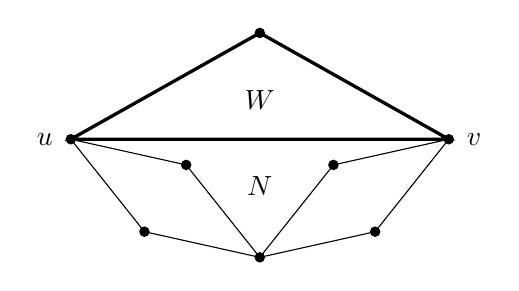
\begin{tikzpicture}
  \coordinate (s) at (0,0);
  \coordinate (t) at (4.8,0);
  \coordinate (m) at (2.4,-1.5);
  \coordinate (w) at (2.4,1.35);
  \coordinate (x1) at (1.465,-0.326);
  \coordinate (y1) at (0.935,-1.174);
  \coordinate (x2) at (3.335,-0.326);
  \coordinate (y2) at (3.865,-1.174);
  \draw (s)--(x1)--(m)--(y1)--cycle;
  \draw (m)--(x2)--(t)--(y2)--cycle;
  \draw[very thick] (s)--(w)--(t)--cycle;
  \foreach \p in {s,t,m,w,x1,y1,x2,y2} \fill (\p) circle (1.9pt);
  \node[left=3pt] at (s) {$u$};
  \node[right=3pt] at (t) {$v$};
  \node at (2.4,0.5) {$W$};
  \node at (2.4,-0.6) {$N$};
\end{tikzpicture}
\caption{The graph of Example~\ref{rem:twoports} for $k=2$: a triangle $W$ (thick) and a chain $N$
of two four-cycles.}
\label{fig:twoports}
\end{figure}



\paragraph{One edge of a cycle.}
The next lemma is the form of the count that Theorem~\ref{thm:sharp} needs. It holds for
multigraphs, with the same proof. For an edge $e$ let $c(G)$ be the number of cycles of $G$ and
$c_e(G)$ the number of cycles of $G$ through $e$. Recall that
$q(G,P)=\PP(\xi\cap E(G-P)\text{ is a forest})$ for a set $P$ of vertices.

\begin{lemma}[Edge recursion]\label{lem:edge}
Let $G$ be a connected graph of rank $r$, let $W$ be a cycle of $G$, and let $e$ be an edge of $W$.
Then $G-e$ is connected and has rank $r-1$, and
\[
  c(G)=c(G-e)+c_e(G),\qquad c_e(G)\;\le\;q\bigl(G,V(W)\bigr)\,2^{r-1}.
\]
\end{lemma}

\begin{proof}
The edge $e$ lies on a cycle, so $G-e$ is connected, and it has one edge less. A cycle of $G$ either
avoids $e$ or contains $e$. This is the first formula.

Let $C$ be a cycle through $e$. Then $C$ and $C+W$ are even subgraphs of $G$. The cycle $C$ has a
vertex in $V(W)$, so $C\cap E(G-V(W))$ is a proper part of a cycle, which is a forest. Every edge of
$W$ has both ends in $V(W)$, so $C+W$ has the same edges in $G-V(W)$ as $C$. The even subgraph $C$
contains $e$, and $C+W$ does not. So if $C'$ is another cycle through $e$, the four sets $C$,
$C+W$, $C'$, $C'+W$ are distinct. Hence there are at least $2c_e(G)$ even subgraphs whose part in
$G-V(W)$ is a forest, and their number is $q(G,V(W))\,2^{r}$.
\end{proof}

In particular, if $q(G,V(W))\le\half+\varepsilon$, then
$c(G)\le c(G-e)+(\frac14+\frac\varepsilon2)2^{r}$. For a graph with the largest number of cycles
this reads $\psi(r)\le\psi(r-1)+(\frac14+\frac\varepsilon2)2^{r}$. If $\varepsilon$ is zero, the
difference $\psi(r)-2^{r-1}$ does not grow at all in this step.

\section{The number of cycles}\label{sec:cycles}

This section proves Theorem~\ref{thm:cycles}. The main step is Lemma~\ref{lem:through}.
Appendix~\ref{app:lean} names the Lean declaration for each step.

\subsection{The lower bound}

Entringer and Slater proved that $\psi(r)>2^{r-1}$ for $r\ge3$. Their examples are cubic: a cycle of
even length with all its long diagonals. These graphs give
$\psi(r)\ge2^{r-1}+r^{2}-3r+3$~\cite[Corollary~4]{ES}.

A simpler example suffices here. Let $j\ge2$. Take vertices $u_1,\dots,u_j$ and, for each $i$, two
further vertices $x_i$ and $y_i$ that are joined to $u_i$ and to $u_{i+1}$, with indices modulo $j$.
This is a ring of $j$ four-cycles: a chain like $N$ in Figure~\ref{fig:twoports}, closed up. It has
$3j$ vertices and $4j$ edges, so its rank is $j+1$. Its cycles are the $j$ four-cycles and the
$2^{j}$ cycles that pass through all the vertices $u_i$. So $\psi(r)\ge2^{r-1}+r-1$ for $r\ge3$.
The formal proof uses a closed chain of shortcuts from the construction of
Section~\ref{sec:upper} instead, which has rank $j+1$ and at least $2^{j}$ cycles.

\subsection{The upper bound}

In this subsection $G$ is a connected simple graph of rank $r$, and $k$ is an integer with
$1\le k\le r$.

\begin{lemma}[Independent edges]\label{lem:indep}
There is a set $D$ of $k$ edges of $G$ such that exactly $2^{r-k}$ even subgraphs of $G$ contain no
edge of $D$. Every edge of $D$ lies on a cycle of $G$.
\end{lemma}

\begin{proof}
Fix a spanning tree of $G$. Exactly $r$ edges of $G$ lie outside the tree. Let $D$ consist of $k$
of them. The graph $G-D$ contains the tree, so it is connected, and its rank is $r-k$. The even
subgraphs of $G$ that contain no edge of $D$ are the even subgraphs of $G-D$. So there are
$2^{r-k}$ of them. An edge of $D$ lies on a cycle, because the tree contains a path between its
ends.
\end{proof}

\paragraph{Chords and triangles.}
Let $e=uv$ be an edge of $D$. It lies on a cycle, so $v$ has a neighbour $w_e\ne u$. Fix such a
neighbour for each edge of $D$. If $u$ and $w_e$ are not adjacent in $G$, add the edge $uw_e$ and
call it a \emph{chord} (Figure~\ref{fig:chord}). Let $G^{+}$ be the graph that we get when we add
all chords, each of them once, and let $a\le k$ be the number of chords. The graph $G^{+}$ is simple
and connected, and it has the same vertices as $G$. So $\beta(G^{+})=r+a$.

For $e\in D$ let $T_e$ be the triangle of $G^{+}$ with the edges $uv$, $vw_e$ and $uw_e$, and let
$W$ be the union of these triangles. Then $W$ is a nonempty union of cycles of $G^{+}$, with at most
$3k$ edges and at most $k$ components. It contains every edge of $D$ and every chord. Every chord
$f$ lies on a triangle $T_f$ of $W$ whose other two edges are edges of $G$. If there are several
such triangles, fix one of them.

\begin{figure}[ht]
\centering
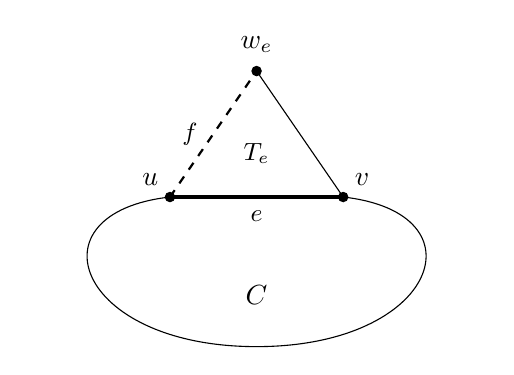
\begin{tikzpicture}
  \coordinate (u) at (0,0);
  \coordinate (v) at (2.2,0);
  \coordinate (w) at (1.1,1.6);
  \draw (v) .. controls (4.0,-0.2) and (3.4,-1.9) .. (1.1,-1.9)
            .. controls (-1.2,-1.9) and (-1.8,-0.2) .. (u);
  \draw[very thick] (u) -- node[below=1pt] {\small$e$} (v);
  \draw (v) -- (w);
  \draw[dashed,thick] (u) -- node[left=2pt] {\small$f$} (w);
  \foreach \p in {u,v,w} \fill (\p) circle (1.9pt);
  \node[above left=1pt] at (u) {$u$};
  \node[above right=1pt] at (v) {$v$};
  \node[above=3pt] at (w) {$w_e$};
  \node at (1.1,-1.25) {$C$};
  \node at (1.1,0.55) {\small$T_e$};
\end{tikzpicture}
\caption{An edge $e=uv$ of $D$, a second neighbour $w_e$ of $v$, and the chord $f=uw_e$ (dashed).
The chord is added if $u$ and $w_e$ are not adjacent in $G$. A cycle $C$ through $e$ and the even
subgraph $C+T_e$ have the same edges outside the triangle $T_e$.}
\label{fig:chord}
\end{figure}

\begin{lemma}[Cycles through $D$]\label{lem:through}
At most $p(G^{+},W)\,2^{r}$ cycles of $G$ contain an edge of $D$.
\end{lemma}

\begin{proof}
Let $F$ be the set of chords, so $|F|=a$. For a cycle $C$ of $G$ that contains an edge of $D$, and
for a set $S\subseteq F$, put
\[
  C_S=C+\sum_{f\in S}T_f .
\]
This is an even subgraph of $G^{+}$. We show two things.

\emph{The outside part of $C_S$ is a forest.} All triangles lie in $W$, so
$C_S\sm E(W)=C\sm E(W)$. The cycle $C$ contains an edge of $D$, and $D\subseteq E(W)$. So
$C\sm E(W)$ is a forest by Lemma~\ref{lem:count}(a).

\emph{The even subgraph $C_S$ determines the pair $(C,S)$.} The cycle $C$ contains no chord. The
triangle $T_f$ contains the chord $f$ and no other chord. So the set of chords in $C_S$ is $S$. Thus
$C_S$ determines $S$, and then it determines $C=C_S+\sum_{f\in S}T_f$.

Let $q$ be the number of cycles of $G$ that contain an edge of $D$. The sets $C_S$ are $q\,2^{a}$
distinct even subgraphs of $G^{+}$ whose outside part is a forest. By~\eqref{eq:count}, applied to
$G^{+}$ and $W$, there are exactly $p(G^{+},W)\,2^{r+a}$ such even subgraphs. Hence
$q\le p(G^{+},W)\,2^{r}$.
\end{proof}

\begin{proof}[Proof of Theorem~\ref{thm:cycles}]
Let $G$ be a graph of rank $r$, where $r$ is large. If $G$ is not connected, add a new vertex and
join it to one vertex of each component. The new edges are bridges, so the rank and the set of
cycles do not change. So we may assume that $G$ is connected.

Let $k$ be the least integer with $2^{k}>\log r$. Then $k\le\log\log r+1$, and $1\le k\le r$. Take
$D$ as in Lemma~\ref{lem:indep}, and take $G^{+}$ and $W$ as above. A cycle of $G$ avoids $D$ or
contains an edge of $D$. At most $2^{r-k}<2^{r}/\log r$ cycles avoid $D$, by
Lemma~\ref{lem:indep}. At most $p(G^{+},W)\,2^{r}$ cycles contain an edge of $D$, by
Lemma~\ref{lem:through}.

It remains to bound $p(G^{+},W)$. The graph $G^{+}$ is connected and simple, and its rank
$r^{+}=r+a$ is at least $r$. The subgraph $W$ is a nonempty union of cycles. It has at most
$3k\le\sqrt{r}\le\sqrt{r^{+}}$ edges and at most $k\le(\log r)/100\le(\log r^{+})/100$ components,
because $r$ is large. So Theorem~\ref{thm:forest} applies to $G^{+}$ and $W$, and
\[
  p(G^{+},W)\;\le\;\frac12+\frac{20}{\lgk3r^{+}}\;\le\;\frac12+\frac{20}{\lgk3r}.
\]
Altogether, the number of cycles of $G$ is at most
\[
  \Bigl(\frac12+\frac{20}{\lgk3r}+\frac1{\log r}\Bigr)2^{r}
  \;\le\;\Bigl(\frac12+\frac{21}{\lgk3r}\Bigr)2^{r},
\]
because $\lgk3r\le\log r$. Together with the lower bound, this gives $\psi(r)\sim2^{r-1}$.
\end{proof}

\begin{remark}\label{rem:chords}
The choice of $k$ is not delicate. The proof needs $2^{-k}\le1/\lgk3r$ for the cycles that avoid
$D$, and $100k\le\log r$ for the components of $W$.

The chords are the point of the proof. Without them one would take for $W$ a union of cycles of $G$
through the edges of $D$. Such cycles can be long, and Theorem~\ref{thm:forest} needs $W$ to be
small. To shorten them one would have to pass to a cubic multigraph and search for short cycles
there. The chords create the short cycles directly, and Lemma~\ref{lem:through} shows that they cost
nothing.
\end{remark}

\section{The lower bound for pancyclic graphs}\label{sec:lower}

This section derives the lower bound of Theorem~\ref{thm:main} from Theorem~\ref{thm:forest}. The
plan is as follows. A number $\Phi(R)\le1$ measures how well a graph of rank at least $R$ can fill
an interval of cycle lengths. In a graph with many cycle lengths we find a small subgraph $W$ that
already contains the short cycles. The forest estimate for $W$ then shows that $\Phi$ drops by a
factor of almost two when the rank grows from $R$ to $2^{256R}$.

For an integer $R\ge1$ let
\[
  \Phi(R)=\sup\,\frac{L-2}{2^{\beta(G)}} ,
\]
where the supremum is over all simple graphs $G$ with $\beta(G)\ge R$ and all integers $L\ge2$ such
that $G$ contains a cycle of each length $3,\dots,L$. A graph of rank $\beta$ has at most
$2^{\beta}-1$ cycles, so $\Phi(R)\le1$. The function $\Phi$ is non-increasing, because a larger $R$
allows fewer graphs.

\begin{lemma}[Witness]\label{lem:witness}
Let $R\ge1$ and $\varphi=\Phi(R)$, and let $G$ contain a cycle of each length $3,\dots,L$, where
$L\ge2^{2R}$. Then $G$ has a subgraph $W$ that is a union of at most $2R$ cycles, with
$\beta(W)\ge2R$ and $|E(W)|\le\varphi\,2^{2R}+2^{R}+5R$.
\end{lemma}

\begin{proof}
Put $W_0=\emptyset$ and $W_{i+1}=W_i\cup C_i$, where $C_i$ is a cycle of $G$ whose length $\ell_i$ is
the least integer $\ge3$ that is not the length of a cycle of $W_i$. Stop as soon as the rank is at
least $2R$. Consider a step, and let $s=\beta(W_i)<2R$. The graph $W_i$ contains cycles of the
$\ell_i-3$ lengths $3,\dots,\ell_i-1$. Therefore $\ell_i-3\le2^{s}-1$. This gives
$\ell_i\le2^{2R-1}+2\le L$, so $C_i$ exists. If $s\ge R$, then also $\ell_i-3\le\varphi\,2^{s}$, by
the definition of $\Phi$. The cycle $C_i$ is not a subgraph of $W_i$, so the rank increases at every
step. So there are at most $2R$ steps, their ranks $s$ are distinct, and
\[
  |E(W)|\;\le\;\sum_i\ell_i\;\le\;\sum_{s=0}^{R-1}\bigl(2^{s}+2\bigr)+\sum_{s=R}^{2R-1}\bigl(\varphi\,2^{s}+3\bigr)
  \;\le\;\varphi\,2^{2R}+2^{R}+5R .\qedhere
\]
\end{proof}

\begin{proposition}[Near-halving]\label{prop:halving}
For every sufficiently large integer $R$,
\[
  \Phi\bigl(2^{256R}\bigr)\;\le\;\Bigl(\frac12+\frac{20}{\lgk{2}R}\Bigr)\Phi(R)+2^{2-R}.
\]
\end{proposition}

\begin{proof}
Let $G$ be a simple graph of rank $r\ge2^{256R}$ with a cycle of each length $3,\dots,L$. We bound
$(L-2)\,2^{-r}$. Identifying a vertex of one component with a vertex of another changes neither the
rank nor the set of cycles, so we may assume that $G$ is connected. If $L<2^{2R}$, then
$(L-2)\,2^{-r}<2^{2-R}$, and we are done.

Otherwise let $W$ be as in Lemma~\ref{lem:witness}, with $m$ edges and rank $t\ge2R$, and let
$\varphi=\Phi(R)$. Then $m\le2^{2R+1}\le\sqrt r$ and $\comp(W)\le2R\le(\log r)/100$. This is
the only place in this proof where the size of the exponent $256$ matters, and any exponent of at
least $200$ would do.
So Theorem~\ref{thm:forest} gives
\[
  p(G,W)\;\le\;\frac12+\frac{20}{\lgk3r}\;\le\;\frac12+\delta,
  \qquad\text{where }\delta=\frac{20}{\lgk2R}.
\]
The second inequality holds because $\lgk3r\ge\log(8+\log R)\ge\lgk2R$. The graph $G$ has cycles of
at least $L-2$ lengths. So Lemma~\ref{lem:count}(b), with $p=p(G,W)$, and the bounds on $t$ and $m$
give
\[
  \frac{L-2}{2^{r}}\;\le\;\frac{pm+1}{2^{t}}
  \;\le\;\Bigl(\frac12+\delta\Bigr)\bigl(\varphi+2^{-R}+5R\,2^{-2R}\bigr)+2^{-2R}
  \;\le\;\Bigl(\frac12+\delta\Bigr)\varphi+2^{2-R}.\qedhere
\]
\end{proof}

\begin{corollary}\label{cor:phi}
There is a constant $c$ such that $\Phi(r)\le c\,2^{-\lgs r}$ for all $r\ge1$.
\end{corollary}

\begin{proof}
Fix $R_0\ge512$ so large that Proposition~\ref{prop:halving} holds for all $R\ge R_0$. Let
$R_{j+1}=2^{256R_j}$ and $\delta_j=20/\lgk2R_j$. By Proposition~\ref{prop:halving}, the numbers
$a_j=2^{j}\Phi(R_j)$ satisfy
\[
  a_{j+1}\;\le\;(1+2\delta_j)\,a_j+2^{\,j+3-R_j}.
\]
For $j\ge2$ we have $\lgk2R_j=8+256R_{j-2}$, so $\sum_j\delta_j<\infty$. Also
$\sum_j2^{\,j-R_j}<\infty$. Hence the numbers $a_j$ are bounded, say $\Phi(R_j)\le c_1 2^{-j}$.

The numbers $R_j$ grow like a tower of exponentials. To bound $\lgs R_j$, we compare them with an
exact tower. Let $U_0=R_0^2$ and $U_{j+1}=2^{U_j}$, so that $\lgs U_j=j+\lgs U_0$. Then
$R_j\le\sqrt{U_j}$ for all $j$. Indeed, if this holds for $j$, then
\[
  R_{j+1}=2^{256R_j}\;\le\;2^{256\sqrt{U_j}}\;\le\;2^{U_j/2}=\sqrt{U_{j+1}},
\]
because $\sqrt{U_j}\ge R_0\ge512$. Hence $\lgs R_j\le j+\lgs U_0$.

Finally let $r\ge R_0$, and let $j$ be largest with $R_j\le r$. Then
$\Phi(r)\le\Phi(R_j)\le c_12^{-j}$ and $\lgs r\le\lgs R_{j+1}\le j+1+\lgs U_0$. Together these give
$\Phi(r)\le c\,2^{-\lgs r}$ with $c=c_1\,2^{1+\lgs U_0}$. For $r<R_0$ use $\Phi(r)\le1$, and enlarge
$c$ if necessary.
\end{proof}

\begin{proof}[Proof of the lower bound in Theorem~\ref{thm:main}]
Let $G$ be a pancyclic graph with $n$ vertices and $n+h$ edges. It is connected, so its rank is
$r=h+1$. By the definition of $\Phi$ and by Corollary~\ref{cor:phi},
\[
  n-2\;\le\;\Phi(r)\,2^{r}\;\le\;c\,2^{\,r-\lgs r}.
\]
We compare $\lgs r$ with $\lgs n$. The trivial bound $n-2\le2^{r}-1$ gives
$n\le2^{r+1}\le2^{2^{r}}$, hence $\lgs n\le\lgs r+2$. Now take logarithms in the display:
\[
  h=r-1\;\ge\;\log(n-2)+\lgs r-\log c-1\;\ge\;\log n+\lgs n-\log c-5.\qedhere
\]
\end{proof}

\paragraph{Formal counterpart.}
In the Lean code $\Phi$ is \lean{actualRankTail}. Proposition~\ref{prop:halving} is
\lean{ShortProof.recurrence_of_few_component_forest_estimate}, with the same constants.
Corollary~\ref{cor:phi} is an instance of \lean{recurrence_logStar_bound}. Lemma~\ref{lem:witness}
corresponds to \lean{ShortProof.exists_budgeted_witness}, where the bookkeeping differs in detail.

\section{The construction}\label{sec:upper}

This section proves the upper bound of Theorem~\ref{thm:main}. The construction follows~\cite{KNT}.
It is a chain of beads. Bead $i$ can be passed in two ways, and the two ways differ in length by
$2^{i}$. So $k$ beads give $2^{k}$ consecutive path lengths for the price of $k$ chords. A few more
chords close shorter and shorter parts of the chain, and these supply the short cycles.

\begin{proposition}\label{prop:upper}
For every $n\ge3$ there is a pancyclic graph with $n$ vertices and at most
$n+\lfloor\log n\rfloor+\lgs n+1$ edges.
\end{proposition}

\begin{proof}
For $3\le n\le6$ take a cycle $u_0u_1\cdots u_{n-1}$, with the chord $u_0u_2$ if $n\ge4$ and also
the chord $u_0u_3$ if $n=6$. Now let $n\ge7$.

\emph{The necklace.} Let $k\ge2$ be the largest integer with $2^{k}+k+1\le n$, so that
$n\le2^{k+1}+k+1$. Let $H$ be a cycle of length $n$, and let $Q\subseteq H$ be a path that is
composed of consecutive segments $Q_0,\dots,Q_{k-1}$, where $Q_i$ has $2^{i}+1$ edges and joins
$v_i$ to $v_{i+1}$. Thus $Q$ has $2^{k}+k-1\le n-2$ edges. Add the chords $e_i=v_iv_{i+1}$ for
$0\le i<k$. For $1\le j\le k$ let $N_j$, the \emph{necklace with $j$ beads}, be the union of
$Q_0,\dots,Q_{j-1}$ and $e_0,\dots,e_{j-1}$ (Figure~\ref{fig:necklace}).

A path from $v_0$ to $v_j$ in $N_j$ uses either $Q_i$ or $e_i$ for each $i<j$, and it is shorter by
$2^{i}$ if it uses $e_i$. So $N_j$ has $2^{j}$ such paths, exactly one of each length from $j$ to
$2^{j}+j-1$. The rest $H-Q$ of the outer cycle is a path from $v_k$ to $v_0$ with $n-2^{k}-k+1$
edges. Together with $N_k$ it contains a cycle of each length in the interval
\[
  [\,n-2^{k}+1,\ n\,].
\]

\emph{Closing chords.} For $2\le j\le k$ the chord $f_j=v_0v_j$ closes the paths of $N_j$ to cycles
of all lengths in the interval
\[
  I_j=[\,j+1,\ 2^{j}+j\,].
\]
Add the chord $f_j$ for $j=k$, then for $j=\lceil\log k\rceil$, and so on: as long as the last
value of $j$ is larger than $2$, the next value is $\lceil\log j\rceil$. The last value is $2$. If
$j'=\lceil\log j\rceil$, then $2^{j'}\ge j$, so the intervals $I_{j'}$ and $I_j$ overlap or are
adjacent. Since $I_2=[3,6]$, these chords give a cycle of each length in $[\,3,\ 2^{k}+k\,]$.

\emph{All lengths.} The intervals $[\,3,\ 2^{k}+k\,]$ and $[\,n-2^{k}+1,\ n\,]$ cover all lengths
from $3$ to $n$, except for the length $2^{k}+k+1$ in the case $n=2^{k+1}+k+1$. In that case add
one more chord, which joins $v_k$ to the neighbour of $v_0$ on $H-Q$. This chord, the edge from that
neighbour to $v_0$, and the path $Q$ form a cycle of length $2^{k}+k+1$.

\emph{The number of chords.} For an integer $j\ge3$ we have $\lgs\lceil\log j\rceil=\lgs j-1$, and
$\lgs2=1$. So exactly $\lgs k$ chords $f_j$ were added. The number of all chords is therefore at
most $k+\lgs k+1\le\lfloor\log n\rfloor+\lgs n+1$.
\end{proof}

\begin{figure}[ht]
\centering
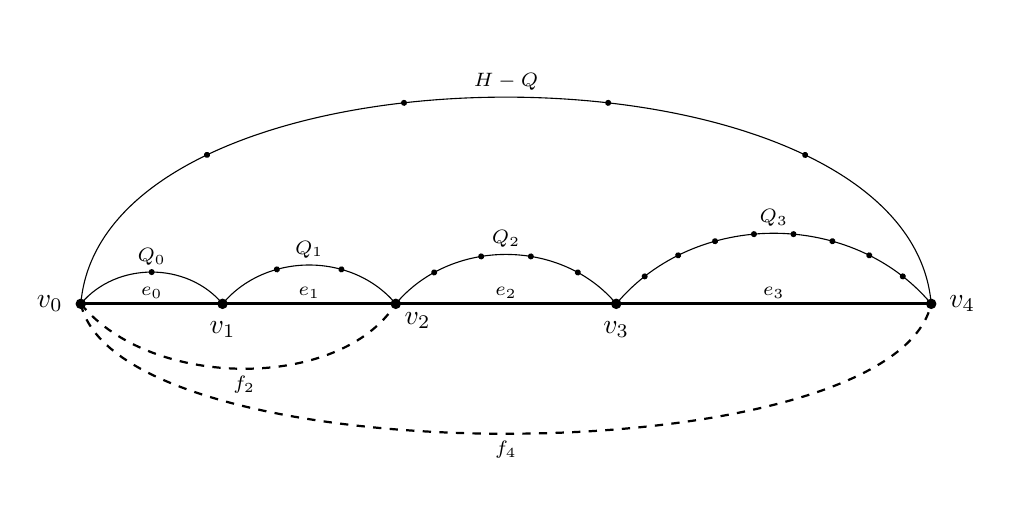
\begin{tikzpicture}[
  iv/.style 2 args={postaction={decorate,decoration={markings,
      mark=between positions #1 and #2 step #1 with {\fill (0,0) circle (1.1pt);}}}}]
  \coordinate (v0) at (0,0);
  \coordinate (v1) at (1.8,0);
  \coordinate (v2) at (4.0,0);
  \coordinate (v3) at (6.8,0);
  \coordinate (v4) at (10.8,0);
  \draw[iv={0.5}{0.51}]    (v0) to[bend left=50] node[pos=0.5,above=-1pt] {\scriptsize$Q_0$} (v1);
  \draw[iv={0.3333}{0.67}] (v1) to[bend left=50] node[pos=0.5,above=-1pt] {\scriptsize$Q_1$} (v2);
  \draw[iv={0.2}{0.81}]    (v2) to[bend left=50] node[pos=0.5,above=-1pt] {\scriptsize$Q_2$} (v3);
  \draw[iv={0.1111}{0.89}] (v3) to[bend left=50] node[pos=0.5,above=-1pt] {\scriptsize$Q_3$} (v4);
  \draw[iv={0.2}{0.81}]    (v0) .. controls (0.3,3.5) and (10.5,3.5) .. node[pos=0.5,above=-1pt] {\scriptsize$H-Q$} (v4);
  \foreach \a/\b/\i in {v0/v1/0,v1/v2/1,v2/v3/2,v3/v4/3}
    \draw[very thick] (\a) -- node[pos=0.5,above=-2pt] {\scriptsize$e_{\i}$} (\b);
  \draw[thick,dashed] (v0) .. controls (0.9,-1.1) and (3.3,-1.1) .. node[pos=0.5,below=-1pt] {\scriptsize$f_2$} (v2);
  \draw[thick,dashed] (v0) .. controls (0.5,-2.2) and (10.3,-2.2) .. node[pos=0.5,below=-1pt] {\scriptsize$f_4$} (v4);
  \foreach \p in {v0,v1,v2,v3,v4} \fill (\p) circle (1.9pt);
  \node[left=3pt] at (v0) {$v_0$};
  \node[below=3pt] at (v1) {$v_1$};
  \node[anchor=north west,inner sep=3pt] at (v2) {$v_2$};
  \node[below=3pt] at (v3) {$v_3$};
  \node[right=3pt] at (v4) {$v_4$};
\end{tikzpicture}
\caption{The construction for $n=24$, where $k=4$. The segments $Q_0,\dots,Q_3$ of the outer cycle
$H$ have $2,3,5,9$ edges and are doubled by the chords $e_0,\dots,e_3$. The chord $f_4$ gives the
cycle lengths $5,\dots,20$, the rest $H-Q$ of the outer cycle gives $9,\dots,24$, and $f_2$ gives
$3,\dots,6$.}
\label{fig:necklace}
\end{figure}

\paragraph{Formal counterpart.}
The Lean theorem \lean{Problem1016.upper_bound_integer} states that
$h(n)\le\lfloor\log n\rfloor+\lgs n+1$ for every $n\ge3$. Its proof formalises the construction
of~\cite{KNT}. The proof above describes that construction in our own words. As a check on the
wording, we built the graph of this section by computer for all $n\le139$ and for eight larger
values up to $522$. Each of these graphs is pancyclic and has at most the stated number of edges
(Appendix~\ref{app:checks}).

\section{Proof of the forest estimate}\label{sec:forest}

This section proves Theorem~\ref{thm:forest}. The argument is that of~\cite{KNT}. It has five steps.
\begin{enumerate}
\item \emph{Cuts.} For a set $A$ of vertices, consider the event that $\xi$ avoids every edge that
leaves $A$. Its probability is explicit. For two disjoint sets the two events are correlated by the
factor $2^{\ell-1}$, where $\ell$ counts the links between the sets (Lemma~\ref{lem:link}). One link
means independence, and two links mean a factor of two.
\item \emph{Reduction.} We pass to a graph $\Gamma$ with all degrees at most $3$, in which $W$ has
become a small set $P$ of vertices (Lemma~\ref{lem:reduce}).
\item \emph{Short cycles.} Step~1 and a second moment bound show that many disjoint short cycles in
$\Gamma-P$ already force the estimate (Lemma~\ref{lem:smallcuts}). So we may delete a small maximal
family of them, and we are left with a graph $J$ of large girth.
\item \emph{Supply.} The graph $J$ has many cycles with between $6\log r$ and
$\log r\sqrt{\log\log r}$ edges. Their total weight $\sum_C2^{-|C|}$ is at least
$(\frac18-o(1))\ln\log\log r$ (Lemma~\ref{lem:weight}). This step uses the non-backtracking matrix.
\item \emph{Second moment.} For such a cycle $C$, the event that $C$ is a component of $\xi$ has
probability at least $2^{-|C|}$. If it occurs, then the part of $\xi$ outside $P$ is not a forest.
We weight the indicators of these events so that their means are exactly $2^{-|C|}$. Most pairs of
the events are correlated by a factor of at most two.
\end{enumerate}
The factor two in step~5 is the source of the constant $\half$. Lemma~\ref{lem:second} turns the
bound $\EE Z^{2}\le2\mu^{2}+K\mu$ into $\PP(Z=0)\le\half+K/(4\mu)$. Appendix~\ref{app:lean} lists the
Lean declarations that correspond to the steps.

In this section graphs may have loops and parallel edges. A loop adds two to the degree of its vertex
and is a cycle of length one. Two parallel edges form a cycle of length two. For a set $A$ of
vertices of $G$ we write $G[A]$ for the induced subgraph, $G-A$ for $G[V(G)\sm A]$, and $\delta A$
for the set of edges with exactly one end in $A$. A \emph{region} is a nonempty set $A$ such that
$G[A]$ is connected. A region is \emph{cyclic} if $G[A]$ contains a cycle. As before $\xi$ is
uniform on $\Z(G)$, and $\cO_A$ denotes the event $\xi\cap\delta A=\emptyset$.

\subsection{Cuts and links}

\begin{lemma}\label{lem:second}
Let $Z\ge0$ be a random variable with $\mu=\EE Z>0$ and $\EE Z^{2}\le2\mu^{2}+K\mu$. Then
$\PP(Z=0)\le\half+K/(4\mu)$.
\end{lemma}

\begin{proof}
By the Cauchy--Schwarz inequality $\mu^{2}\le\EE Z^{2}\cdot\PP(Z>0)$, so
$\PP(Z=0)\le1-\mu/(2\mu+K)\le\half+K/(4\mu)$.
\end{proof}

Let $A$ and $B$ be disjoint regions of a connected graph $G$. A \emph{link} between them is an edge
with one end in $A$ and the other in $B$, or a component of $G-(A\cup B)$ that is joined by an edge
to $A$ and by an edge to $B$ (Figure~\ref{fig:links}). Let $\ell(A,B)$ be the number of links.

\begin{figure}[ht]
\centering
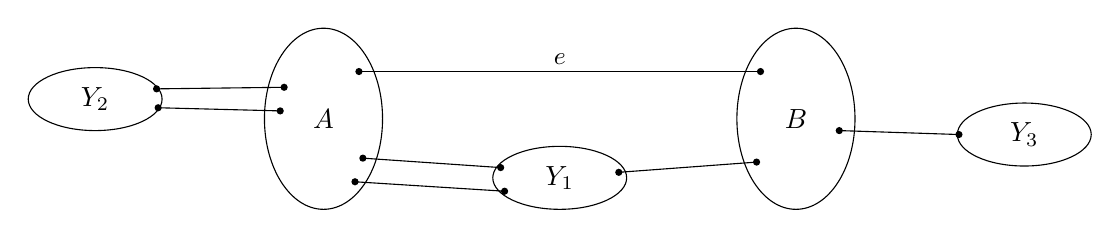
\begin{tikzpicture}
  \draw (0,0) ellipse [x radius=0.75, y radius=1.15];
  \draw (6,0) ellipse [x radius=0.75, y radius=1.15];
  \draw (3,-0.75) ellipse [x radius=0.85, y radius=0.4];
  \draw (-2.9,0.25) ellipse [x radius=0.85, y radius=0.4];
  \draw (8.9,-0.2) ellipse [x radius=0.85, y radius=0.4];
  \node at (0,0) {$A$};
  \node at (6,0) {$B$};
  \node at (3,-0.75) {$Y_1$};
  \node at (-2.9,0.25) {$Y_2$};
  \node at (8.9,-0.2) {$Y_3$};
  \draw (0.45,0.6) -- node[above=-1pt] {\small$e$} (5.55,0.6);
  \draw (0.5,-0.5) -- (2.25,-0.62);
  \draw (0.4,-0.8) -- (2.3,-0.92);
  \draw (5.5,-0.55) -- (3.75,-0.68);
  \draw (-0.5,0.4) -- (-2.12,0.38);
  \draw (-0.55,0.1) -- (-2.1,0.14);
  \draw (6.55,-0.15) -- (8.07,-0.2);
  \foreach \p in {(0.45,0.6),(5.55,0.6),(0.5,-0.5),(2.25,-0.62),(0.4,-0.8),(2.3,-0.92),(5.5,-0.55),
                  (3.75,-0.68),(-0.5,0.4),(-2.12,0.38),(-0.55,0.1),(-2.1,0.14),(6.55,-0.15),(8.07,-0.2)}
    \fill \p circle (1.3pt);
\end{tikzpicture}
\caption{Links between two regions $A$ and $B$. The edge $e$ and the component $Y_1$ of
$G-(A\cup B)$ are links. The components $Y_2$ and $Y_3$ are joined to one region only, so they are
not links. Here $\ell(A,B)=2$. In the proof of Lemma~\ref{lem:link} this is the case $a=b=k=1$
and $e(A,B)=1$.}
\label{fig:links}
\end{figure}

\begin{lemma}[Link formula]\label{lem:link}
Let $A$ and $B$ be disjoint regions of a connected graph $G$. Then
$\PP(\cO_A)=2^{\comp(G-A)-|\delta A|}\ge2^{-|\delta A|}$ and
\[
  \PP(\cO_A\cap\cO_B)=2^{\ell(A,B)-1}\,\PP(\cO_A)\,\PP(\cO_B).
\]
Conditionally on $\cO_A$, the set $\xi\cap E(G[A])$ is uniform on $\Z(G[A])$; conditionally on
$\cO_A\cap\cO_B$, the sets $\xi\cap E(G[A])$ and $\xi\cap E(G[B])$ are independent and uniform on
$\Z(G[A])$ and $\Z(G[B])$.
\end{lemma}

\begin{proof}
The even subgraphs that avoid $\delta A$ are the sums of an even subgraph of $G[A]$ and an even
subgraph of $G-A$. So $\PP(\cO_A)=2^{\beta(G[A])+\beta(G-A)-\beta(G)}$, and counting edges and
vertices shows that the exponent is $\comp(G-A)-|\delta A|$. In the same way
\[
  \PP(\cO_A\cap\cO_B)=2^{\beta(G[A])+\beta(G[B])+\beta(G-A-B)-\beta(G)}
     =2^{\comp(G-A-B)+1-|\delta A|-|\delta B|+e(A,B)},
\]
where $e(A,B)$ is the number of edges between $A$ and $B$. Let $a$, $b$ and $k$ be the numbers of
components of $G-A-B$ that are joined to $A$ only, to $B$ only, and to both. Then
$\comp(G-A-B)=a+b+k$, while $\comp(G-A)=a+1$ and $\comp(G-B)=b+1$, and the formula follows since
$\ell(A,B)=k+e(A,B)$. The conditional laws are read off from the two direct sum decompositions.
\end{proof}

So two cut events are independent when there is one link. They are correlated by a factor of
exactly two when there are two links. The correlation is stronger only for pairs with at least
three links, and the next lemma says that such pairs are rare.

\begin{lemma}[Exceptional partners]\label{lem:exc}
Let $A$ be a region of a connected graph $G$, and let $B_1,\dots,B_k$ be pairwise disjoint regions,
disjoint from $A$, with $\ell(A,B_i)\ge3$ for all $i$. Then $k\le|\delta A|$.
\end{lemma}

\begin{proof}
Contract $A$ to a vertex $a$ and each $B_i$ to a vertex $b_i$, and delete the loops that arise.
This changes neither $d=|\delta A|$ nor the numbers $\ell(A,B_i)$, because the sets $B_j$ with
$j\ne i$ are connected and are contracted inside components of $G-(A\cup B_i)$. Let $F$ be a spanning forest of
$G-a$, and for every edge $e=au$ at $a$ attach a new leaf $\tau_e$ to $u$. Call the resulting forest
$F^{+}$ and its $d$ new leaves \emph{terminals}.

Fix $i$. Every link between $a$ and $b_i$ yields a path of $F^{+}$ from $b_i$ to a terminal. For an
edge $e=ab_i$ it is the edge $b_i\tau_e$. For a component $Y$ of $G-\{a,b_i\}$ joined to both, choose
an edge $e=au$ with $u\in Y$ and take the path of $F^{+}$ from $b_i$ to $\tau_e$; after its first
vertex it stays in $Y\cup\{\tau_e\}$. Paths that come from different links therefore start with
different edges at $b_i$, and the union of any two of them is a path between two terminals. Let
$F^{\circ}\subseteq F^{+}$ be the union of all paths between terminals. As $\ell(a,b_i)\ge3$, the
vertex $b_i$ has degree at least $3$ in $F^{\circ}$. All leaves of $F^{\circ}$ are terminals, and a
forest with at most $d$ leaves has at most $d-2$ vertices of degree at least $3$. Hence $k\le d-2$ if $k\ge1$.
\end{proof}

\begin{lemma}[Many small cuts]\label{lem:smallcuts}
Let $A_1,\dots,A_k$ be pairwise disjoint cyclic regions of a connected graph $G$ with
$|\delta A_i|\le d$ for all $i$. Then
\[
  \PP\bigl(\xi\cap E(G[A_i])\text{ is a forest for every }i\bigr)\;\le\;\frac12+\frac{(d+1)\,2^{d-1}}{k}.
\]
\end{lemma}

\begin{proof}
Let $E_i$ be the event that $\cO_{A_i}$ holds and $\xi\cap E(G[A_i])\ne\emptyset$. On $E_i$ the set
$\xi\cap E(G[A_i])$ is a nonempty even subgraph, hence not a forest, so it suffices to bound
$\PP(Z=0)$ for $Z=\sum_i\mathbf{1}_{E_i}$. By Lemma~\ref{lem:link},
$p_i:=\PP(E_i)=\PP(\cO_{A_i})\bigl(1-2^{-\beta(G[A_i])}\bigr)\ge2^{-d-1}$ and
$\PP(E_i\cap E_j)=2^{\ell(A_i,A_j)-1}p_ip_j$ for $i\ne j$. If $\ell(A_i,A_j)\le2$ this is at most
$2p_ip_j$. Otherwise we use $\PP(E_i\cap E_j)\le p_i$; by Lemma~\ref{lem:exc} this happens for at
most $d$ indices $j$, for each $i$. Hence $\EE Z^{2}\le\mu+2\mu^{2}+d\mu$ with
$\mu=\EE Z\ge k\,2^{-d-1}$, and Lemma~\ref{lem:second} gives the claim.
\end{proof}

\subsection{Reduction to a subcubic graph}

\begin{lemma}\label{lem:reduce}
Let $G$ and $W$ be as in Theorem~\ref{thm:forest}, with $m=|E(W)|$ and $c=\comp(W)$. There are a
connected multigraph $\Gamma$ with $\beta(\Gamma)=r$ and all degrees at most $3$, and a set
$P\subseteq V(\Gamma)$, such that
\begin{enumerate}
\item[\textup{(i)}] every vertex outside $P$ has degree $3$, $|P|\le2m$, and $\Gamma[P]$ has at
most $c$ components;
\item[\textup{(ii)}] $p(G,W)\le\PP\bigl(\xi_\Gamma\cap E(\Gamma-P)\text{ is a forest}\bigr)$, where
$\xi_\Gamma$ is uniform on $\Z(\Gamma)$.
\end{enumerate}
In particular $2r-2\le|V(\Gamma)|\le2r+2m$.
\end{lemma}

\begin{proof}
\emph{Splitting.} Replace every vertex $v$ of degree $d\ge4$ by a path $v^{1}v^{2}\cdots v^{d-2}$.
Distribute the $d$ edges at $v$ along this path in some order: two to $v^{1}$, one to each of
$v^{2},\dots,v^{d-3}$, and two to $v^{d-2}$. If $v\in V(W)$, let the edges of $W$ at $v$ come first
in this order, so that they end in an initial segment $v^{1},\dots,v^{i}$ of the path with
$i<\deg_W(v)$. Let $G'$ be the new graph; its degrees are at most $3$. Let $P$ consist of these
initial segments and of the vertices of $W$ that were not split. Then $|P|\le\sum_v\deg_W(v)=2m$,
every edge of $W$ joins two vertices of $P$, and $G'[P]$ has at most $c$ components.

Contracting the new path edges maps $\Z(G')$ bijectively onto $\Z(G)$, so we may take
$\xi_G=\xi_{G'}\cap E(G)$. Every edge of $G'-P$ is a new path edge or an edge of $E(G)\sm E(W)$. If
$\xi_G\sm E(W)$ is a forest, then so is its union with the set of all new path edges, because
contracting these edges, which form a forest, gives back $\xi_G\sm E(W)$. Hence
$p(G,W)\le\PP\bigl(\xi_{G'}\cap E(G'-P)\text{ is a forest}\bigr)$.

\emph{Cleaning.} As long as possible, delete a vertex of degree one outside $P$, or replace a vertex
of degree two outside $P$ and its two edges by a single edge. An even subgraph avoids a pendant edge
and contains both or none of the two edges at a vertex of degree two, so these operations induce
bijections of the cycle spaces. Let $\Gamma$ be the final multigraph. Each edge of $\Gamma-P$ is a
path of $G'$ all of whose vertices lie outside $P$; so if $\xi_\Gamma$ contains a cycle of
$\Gamma-P$, then the corresponding $\xi_{G'}$ contains a cycle of $G'-P$. This proves~(ii).

Edges with both ends in $P$ are never removed, so the vertices of $P$ keep degree at least two, and
the number of components of the graph induced on $P$ does not increase. The vertices outside $P$ now
have degree exactly $3$. Finally $3|V(\Gamma)|-|P|\le2|E(\Gamma)|\le3|V(\Gamma)|$ and
$|E(\Gamma)|=|V(\Gamma)|+r-1$ give the bounds on $|V(\Gamma)|$.
\end{proof}

\subsection{Parameters, and removing the short cycles}

From now on $\Gamma$ and $P$ are as in Lemma~\ref{lem:reduce}, $\xi=\xi_\Gamma$, and $r$ is large.
All $o(\cdot)$ and $O(\cdot)$ refer to $r\to\infty$ and are uniform in $G$ and $W$. Put
\begin{gather*}
  x=\log r,\qquad y=\log x,\qquad z=\log y,\\
  D=\lfloor x/10\rfloor,\qquad L=\lfloor x\sqrt y\rfloor,\qquad
  s=\lfloor(D-1)/2\rfloor,\qquad\varepsilon=20/z .
\end{gather*}
These numbers have the following roles. We delete cycles of length at most $D$, so the graph that
remains has girth greater than $D$. We count cycles of length at most $L$. A non-backtracking walk
of length $s$ in the remaining graph is determined by its two ends. The number $\varepsilon$ is the
error term of the theorem. These letters keep their meaning until the end of the section.

Recall that $|P|\le2\sqrt r$ and $c\le x/100$. Let $\mathcal{F}$ be the event that
$\xi\cap E(\Gamma-P)$ is a forest. We assume that
\begin{equation}\label{eq:assume}
  \PP(\mathcal{F})>\tfrac12+\varepsilon
\end{equation}
and derive a contradiction. By Lemma~\ref{lem:reduce}(ii) this proves Theorem~\ref{thm:forest}.

Let $\mathcal{Q}$ be a maximal family of pairwise disjoint cycles of $\Gamma-P$ of length at most $D$,
loops and pairs of parallel edges included, and let $S$ be the union of their vertex sets. For
$Q\in\mathcal{Q}$ the set $V(Q)$ is a cyclic region of $\Gamma$ with $|\delta V(Q)|\le|Q|\le D$,
because its vertices have degree $3$. On $\mathcal{F}$ the set $\xi\cap E(\Gamma[V(Q)])$ is a forest
for every $Q$, so Lemma~\ref{lem:smallcuts} and~\eqref{eq:assume} give
$|\mathcal{Q}|<(D+1)2^{D-1}/\varepsilon\le\sqrt r$. Hence $|S|\le D\sqrt r$.

Let $J=\Gamma-(P\cup S)$. By the maximality of $\mathcal{Q}$, $J$ is a simple graph of girth greater
than $D$. It has $v=2r+O(\sqrt r\log r)$ vertices, each of degree $3$ in $\Gamma$, so its
\emph{deficit} satisfies
\begin{equation}\label{eq:deficit}
  d_J:=\sum_{u\in V(J)}\bigl(3-\deg_Ju\bigr)\;\le\;3\bigl(|P|+|S|\bigr)=O(\sqrt r\log r).
\end{equation}

\subsection{Cycles of moderate length}

A walk $u_0u_1\cdots u_\ell$ is \emph{non-backtracking} if $u_{i+1}\ne u_{i-1}$ for $0<i<\ell$. Let
$N_\ell(u,w)$ be the number of non-backtracking walks of length $\ell$ from $u$ to $w$ in $J$.

\begin{lemma}\label{lem:walks}
If $\ell>s$, then $N_\ell(u,w)\le3\cdot2^{\ell-s-1}$ for all $u,w$. Consequently, for every vertex
$u$ of $J$, the cycles $C$ of $J$ through $u$ with $|C|\le L$ satisfy $\sum_C2^{-|C|}\le L\,2^{-s}$.
\end{lemma}

\begin{proof}
There are at most $3\cdot2^{\ell-s-1}$ ways to choose the first $\ell-s$ steps. The last $s$ steps
form a non-backtracking walk of length $s$ between two given vertices. Such a walk is a path,
because $s$ is less than the girth, and there is at most one such path, because two of them would
give a cycle of length at most $2s<D$. For the second statement, a cycle of length $\ell$ through $u$
can be traversed from $u$ in two directions, so there are at most $\half N_\ell(u,u)$ of them, and
$\ell>D>s$.
\end{proof}

Let $B$ be the non-backtracking matrix of $J$. Its rows and columns are indexed by the directed
edges $(i\to j)$ of $J$, two for each edge. The entry in row $(i\to j)$ and column $(j'\to k)$ is
$1$ if $j'=j$ and $k\ne i$, and it is $0$ otherwise.

\begin{lemma}\label{lem:spectrum}
For every even $\ell\ge2$,
\[
  \tr B^{\ell}\;\ge\;\bigl(2-d_J/v\bigr)^{\ell}-3v\,2^{\ell/2}.
\]
\end{lemma}

\begin{proof}
Let $A$ be the adjacency matrix of $J$ and $\Delta$ the diagonal matrix of its degrees, and put
$M(\lambda)=\lambda^{2}I-\lambda A+\Delta-I$.

(1) \emph{If $M(\lambda)g=0$ for a real $\lambda>1$ and a vector $g\ne0$, then $\lambda$ is an
eigenvalue of $B$.} A direct computation shows that $f(i\to j)=\lambda g(j)-g(i)$ satisfies
$Bf=\lambda f$; and $f=0$ would give $g(i)=\lambda g(j)=\lambda^{2}g(i)$ along every edge, hence
$g=0$ (at an isolated vertex, $M(\lambda)g=0$ already says $(\lambda^{2}-1)g=0$).

(2) \emph{If $Bf=\lambda f$ with $f\ne0$ and $\lambda^{2}\ne1$, then $M(\lambda)g=0$ for
$g(j)=\sum_{k\sim j}f(j\to k)$, and $g\ne0$.} The eigenvalue equation at $(i\to j)$ and at
$(j\to i)$ reads $\lambda f(i\to j)=g(j)-f(j\to i)$ and $\lambda f(j\to i)=g(i)-f(i\to j)$.
Eliminating $f(j\to i)$ gives $(\lambda^{2}-1)f(i\to j)=\lambda g(j)-g(i)$. This shows that
$g\ne0$. Summing it over the neighbours $j$ of $i$ gives $M(\lambda)g=0$.

(3) \emph{$B$ has a real eigenvalue $\lambda_1\ge2-d_J/v$.} The matrix
$M(2)=2(\Delta-A)+(3I-\Delta)$ is positive semidefinite, while
$\mathbf{1}^{\!\top}M(\lambda)\mathbf{1}=(\lambda-1)(v\lambda-2v+d_J)$ vanishes at
$\lambda^{*}=2-d_J/v>1$. The smallest eigenvalue of the symmetric matrix $M(\lambda)$ is continuous
in $\lambda$, at most $0$ at $\lambda^{*}$ and at least $0$ at $2$. So $M(\lambda_1)$ is singular for
some $\lambda_1\in[\lambda^{*},2]$, and (1) applies.

(4) \emph{Every non-real eigenvalue $\lambda$ of $B$ satisfies $|\lambda|\le\sqrt2$.} With $g$ as
in~(2), $g^{*}M(\lambda)g=0$ is a quadratic equation $a\lambda^{2}-b\lambda+c'=0$ with real
coefficients $a=g^{*}g>0$, $b=g^{*}Ag$ and $c'=g^{*}(\Delta-I)g\le2a$. Its roots are $\lambda$ and
$\bar\lambda$, so $|\lambda|^{2}=c'/a\le2$.

Now $\tr B^{\ell}$ is the sum of the $\ell$th powers of the $2|E(J)|\le3v$ eigenvalues of $B$. For
even $\ell$ the real eigenvalues contribute nonnegative terms, one of which is at least
$(2-d_J/v)^{\ell}$, and the non-real ones contribute at least $-3v\,2^{\ell/2}$ in total.
\end{proof}

Facts (2) and (4) are part of the Ihara--Bass theory~\cite{Bass,KS}. The test vector $\mathbf{1}$
in~(3) is from~\cite{KNT}. It makes the argument work without any assumption of regularity or
expansion.

\begin{lemma}[Cycle weight]\label{lem:weight}
Let $\mathcal{C}$ be the set of cycles of $J$ of length at most $L$. Their total weight satisfies
\[
  \mu:=\sum_{C\in\mathcal{C}}2^{-|C|}\;\ge\;\bigl(\tfrac18-o(1)\bigr)\ln y .
\]
\end{lemma}

\begin{proof}
$\tr B^{\ell}$ is the number of closed walks $u_0u_1\cdots u_\ell=u_0$ in $J$ with
$u_{i+1}\ne u_{i-1}$ for all $i$ modulo $\ell$. A cycle of length $\ell$ gives $2\ell$ of them; let
$n_\ell$ be the number of the others. Then
\[
  T:=\sum_{\ell\le L}\frac{\tr B^{\ell}}{2\ell\,2^{\ell}}=\mu+\sum_{\ell\le L}\frac{n_\ell}{2\ell\,2^{\ell}} .
\]
Consider a walk counted by $n_\ell$, and let $j$ be the least index with
$u_j\in\{u_0,\dots,u_{j-1}\}$, say $u_j=u_i$. Then $j<\ell$, the walk $C=u_iu_{i+1}\cdots u_j$ is a
cycle, of length $q$ say, and $u_ju_{j+1}\cdots u_\ell u_1\cdots u_i$ is a non-backtracking closed
walk of length $\ell-q>0$ from $u_i$ to itself. It contains a cycle, so $\ell-q>D>s$. The original
walk is determined by $C$, by the vertex $u_i$ and a direction on $C$ ($2q$ choices), by the
complementary walk (at most $3\cdot2^{\ell-q-s-1}$ choices, by Lemma~\ref{lem:walks}), and by the
position of $u_0$ on the latter (at most $\ell$ choices). Hence
\[
  \sum_{\ell\le L}\frac{n_\ell}{2\ell\,2^{\ell}}
  \;\le\;\sum_{\ell\le L}\ \sum_{C\in\mathcal{C}}\tfrac32\,|C|\,2^{-|C|-s}
  \;\le\;\tfrac32\,L^{2}\,2^{-s}\,\mu=o(\mu),
\]
because $2^{-s}\le8\,r^{-1/20}$ and $L^{2}\le x^{2}y$.

On the other hand, for even $\ell$ with $6x\le\ell\le L$, Lemma~\ref{lem:spectrum}
and~\eqref{eq:deficit} give
\[
  2^{-\ell}\tr B^{\ell}\;\ge\;\Bigl(1-\frac{d_J}{2v}\Bigr)^{\ell}-3v\,2^{-\ell/2}
  \;\ge\;1-\frac{L\,d_J}{2v}-3v\,r^{-3}=1-o(1).
\]
All terms of $T$ are nonnegative, so $T\ge(1-o(1))\sum1/(2\ell)$ over the even $\ell$ in $[6x,L]$,
and this sum is $(\frac14-o(1))\ln(L/6x)=(\frac18-o(1))\ln y$. Therefore
$\mu=(1-o(1))T\ge(\frac18-o(1))\ln y$.
\end{proof}

\subsection{The second moment}

For $C\in\mathcal{C}$ let $I_C$ be the event that $C$ is a component of $\xi$. As the vertices of
$C$ have degree $3$ in $\Gamma$, this is the event $E(C)\subseteq\xi$. It is also the event that
$\cO_{V(C)}$ holds and $\xi\cap E(\Gamma[V(C)])=E(C)$. Put
\[
  a_C=2^{-|C|},\qquad p_C=\PP(I_C),\qquad X_C=\frac{a_C}{p_C}\,\mathbf{1}_{I_C},\qquad
  Z=\sum_{C\in\mathcal{C}}X_C .
\]
The factor $a_C/p_C$ fixes the mean of $X_C$ at the combinatorial weight $a_C$, whatever the
probability $p_C$ is. We have no upper bound for $p_C$, and with this normalisation we need none.
The event $I_C$ is given by
$|C|$ linear conditions on $\xi\in\Z(\Gamma)$, which are satisfied by $\xi=C$. So $p_C\ge a_C$.
Hence $0\le X_C\le1$, and $\EE Z=\mu$ with $\mu$ as in Lemma~\ref{lem:weight}. On $\mathcal{F}$
no cycle of $J\subseteq\Gamma-P$ is contained in $\xi$, so $Z=0$, and by~\eqref{eq:assume}
\begin{equation}\label{eq:Zzero}
  \PP(Z=0)>\tfrac12+\varepsilon .
\end{equation}

Let $C\ne C'$ be in $\mathcal{C}$. If they share a vertex, then $I_C\cap I_{C'}=\emptyset$. If they
are disjoint, Lemma~\ref{lem:link}, applied to the regions $V(C)$ and $V(C')$ of $\Gamma$, gives
$\PP(I_C\cap I_{C'})=2^{\ell(C,C')-1}p_Cp_{C'}$ and therefore
\begin{equation}\label{eq:pair}
  \EE(X_CX_{C'})=a_Ca_{C'}\,2^{\ell(C,C')-1},
\end{equation}
where $\ell(C,C')$ is the number of links between $V(C)$ and $V(C')$ in $\Gamma$.

\begin{lemma}[Few links]\label{lem:links}
$\ell(C,C')\le c+o(x)$ for all disjoint $C,C'\in\mathcal{C}$.
\end{lemma}

\begin{proof}
Let $U=V(C)\cup V(C')$. Every vertex of $U$ lies on exactly one edge outside its own cycle, so at
most $2L$ edges leave $U$. At most $c$ components of $\Gamma-U$ meet $P$, because $P\cap U=\emptyset$
and so each component of $\Gamma[P]$ lies in one of them. Let $Y$ run over the other components and
let $d_Y$ be the number of edges between $Y$ and $U$; then $\sum_Yd_Y\le2L$. Put
$t_0=\lfloor y/2\rfloor$.

\emph{Large cuts.} At most $2L/t_0$ components have $d_Y>t_0$.

\emph{Small cuts, cyclic.} The components $Y$ with $d_Y\le t_0$ that are cyclic are pairwise
disjoint cyclic regions inside $\Gamma-P$ with $|\delta Y|\le t_0$. On $\mathcal{F}$ each
$\xi\cap E(\Gamma[Y])$ is a forest, so by Lemma~\ref{lem:smallcuts} and~\eqref{eq:assume} there are
fewer than $(t_0+1)2^{t_0-1}/\varepsilon$ of them.

\emph{Small cuts, trees.} Let $Y$ induce a tree, with $d_Y\le t_0$. No $Q\in\mathcal{Q}$ meets $Y$,
since $Q$ is a connected subgraph of $\Gamma-U$ and would lie in $Y$. Hence $Y\subseteq V(J)$. As
all degrees are $3$, we have $3|Y|=2(|Y|-1)+d_Y$, that is, $|Y|=d_Y-2$. So if $Y$ is joined to both
cycles, there is a path $R$ from $C$ to $C'$ through $Y$ with at most $t_0$ edges. For a link that
is an edge, let $R$ be that edge. The paths $R$ obtained in this way lie in $J$ and are pairwise
disjoint. Divide each of $C$ and $C'$ into at most $8L/D$ blocks of at most $D/4$ consecutive
vertices. If two of the paths had their ends in the same block of $C$ and in the same block of $C'$,
they would form, together with two arcs inside these blocks, a cycle of $J$ of length less than
$2t_0+D/2\le D$. So there are at most $(8L/D)^{2}$ such paths.

Altogether
\[
  \ell(C,C')\;\le\;c+\frac{2L}{t_0}+\frac{(t_0+1)2^{t_0-1}}{\varepsilon}+\Bigl(\frac{8L}{D}\Bigr)^{2}
  =c+O\Bigl(\frac{x}{\sqrt y}\Bigr)+O\bigl(yz\sqrt x\bigr)+O(y)=c+o(x).\qedhere
\]
\end{proof}

\begin{proof}[Proof of Theorem~\ref{thm:forest}]
Call a disjoint pair $C,C'\in\mathcal{C}$ \emph{exceptional} if $\ell(C,C')\ge3$. Fix $C$, and let
$\mathcal{E}$ be a maximal family of pairwise disjoint exceptional partners of $C$. By
Lemma~\ref{lem:exc}, $|\mathcal{E}|\le|\delta V(C)|\le L$, so the union $U_C$ of their vertex sets
has at most $L^{2}$ vertices, and every exceptional partner of $C$ meets $U_C$. By
Lemma~\ref{lem:walks}, the sum of $a_{C'}$ over all $C'\in\mathcal{C}$ that meet $U_C$ is at most
$L^{3}2^{-s}$. With~\eqref{eq:pair} and Lemma~\ref{lem:links},
\[
  \sum_{C'\ \mathrm{exceptional}}\EE(X_CX_{C'})\;\le\;a_C\,2^{c+o(x)}L^{3}\,2^{-s}
  =a_C\,2^{\,c-x/20+o(x)}=o(a_C),
\]
because $c\le x/100$.

For the other disjoint pairs $\EE(X_CX_{C'})\le2a_Ca_{C'}$. Intersecting pairs contribute nothing,
and $\EE X_C^{2}\le\EE X_C=a_C$. Summing over $C$ we get
$\EE Z^{2}\le2\mu^{2}+(1+o(1))\mu$. By Lemmas~\ref{lem:second} and~\ref{lem:weight},
\[
  \PP(Z=0)\;\le\;\frac12+\frac{1+o(1)}{4\mu}\;\le\;\frac12+\frac{2+o(1)}{\ln y}\;<\;\frac12+\frac{20}{z}
\]
for large $r$, since $\ln y=z\ln2$. This contradicts~\eqref{eq:Zzero}.
\end{proof}

\begin{remark}\label{rem:range}
The assumption $|E(W)|\le\sqrt r$ entered only through $|P|\le2\sqrt r$ in~\eqref{eq:deficit}, where
all that is needed is $L\,d_J=o(v)$; the proof therefore works unchanged for
$|E(W)|\le r/\log^{2}r$. Similarly the constant $20$ can be replaced by any constant larger than
$2/\ln2$. We have kept the statement of~\cite{KNT}, which is the one that has been formalised.
\end{remark}

\section{The sharp bound: the parts of the proof}\label{sec:sharp}

Sections~\ref{sec:sharp} to~\ref{sec:examples} prove Theorem~\ref{thm:sharp}. This section states
the three parts of the proof and derives the theorem from them. Sections~\ref{sec:affine}
to~\ref{sec:halfproof} prove the first part, Theorem~\ref{thm:half}. Section~\ref{sec:inputs}
describes the other two parts, whose proofs are in the supplement. None of these sections is
formalised as a whole. Table~\ref{tab:sharpsteps} lists the steps that are.

\subsection{Conventions}

As in Section~\ref{sec:forest}, graphs may have loops and parallel edges. A loop adds two to the
degree of its vertex. A loop is a cycle of length one, and two parallel edges form a cycle of
length two. A multigraph is \emph{cubic} if every vertex has degree three, and \emph{subcubic} if
every vertex has degree at most three. The \emph{girth} of a multigraph is the length of a shortest
cycle; a forest has infinite girth. We write $c(G)$ for the number of cycles of $G$.

If we replace an edge by a path, the rank and the number of cycles do not change. So $\psi(r)$ is
also the largest number of cycles of a multigraph of rank $r$.

A \emph{cyclic cut} of $G$ is a set $\delta X$ of edges such that $G[X]$ and $G-X$ each contain a
cycle. Its \emph{size} is $|\delta X|$.

The two auxiliary theorems are stated for cubic multigraphs without loops.

\begin{theorem}[Small cyclic cuts; Astra, supplement~\cite{S1}]\label{thm:smallcut}
There is an absolute constant $K_4$ such that every connected cubic multigraph without loops, of
rank $r$, that has a cyclic cut of size at most four satisfies
\[
  c(G)\;\le\;2^{r-1}+K_4\,r\,2^{r/2}.
\]
\end{theorem}

\begin{theorem}[Bounded girth; Astra, supplement~\cite{S2}]\label{thm:girth}
For every integer $g_0\ge2$ there is $R(g_0)$ with the following property. Let $G$ be a connected
cubic multigraph without loops, of rank $r\ge R(g_0)$ and girth at most $g_0$, that has no cyclic
cut of size at most four. Then $c(G)<2^{r-1}$.
\end{theorem}

The graphs of Horak and Kim have cyclic cuts of size four, and they have more than $2^{r-1}$
cycles. So the second term of Theorem~\ref{thm:sharp} comes from Theorem~\ref{thm:smallcut} alone.
In the other two cases the proof gives no excess over $2^{r-1}$ beyond the excess at smaller rank.

\subsection{Cubic graphs}

\begin{lemma}\label{lem:cubic}
For every $r\ge2$ there is a connected cubic multigraph of rank $r$ with exactly $\psi(r)$ cycles.
\end{lemma}

\begin{proof}
The numbers of cycles of the graphs of rank $r$ are integers below $2^{r}$, so some graph $G_0$
attains $\psi(r)$. If $G_0$ is not connected, identify a vertex of one component with a vertex of
another. This changes neither the rank nor the set of cycles. Now delete a vertex of degree one, or
replace a vertex of degree two and its two edges by one edge, as long as this is possible. These
steps keep the rank and the number of cycles. They may produce loops and parallel edges. The result
is a connected multigraph with all degrees at least three, because $r\ge2$.

Let $v$ be a vertex of degree $d\ge4$. Replace $v$ by a path $v^{1}v^{2}\cdots v^{d-2}$, and
distribute the $d$ edge ends at $v$ along this path: two at $v^{1}$, one at each of
$v^{2},\dots,v^{d-3}$, and two at $v^{d-2}$. The new multigraph has $d-3$ more vertices and $d-3$
more edges, so its rank is $r$. A cycle through $v$ uses two edge ends at $v$. Together with the
part of the path between these two ends it is a cycle of the new multigraph. Different cycles give
different cycles, and the cycles that avoid $v$ remain. So the number of cycles does not decrease,
and it cannot increase beyond $\psi(r)$. Repeat this for every vertex of degree at least four.
\end{proof}

Entringer and Slater proved the same statement with simple cubic graphs for $r\ge3$~\cite{ES}. We
do not need it in that form.

\subsection{Proof of Theorem~\ref{thm:sharp}}

The lower bound for $\psi(r)$ is~\eqref{eq:hk}; Section~\ref{sec:examples} recalls the graphs.
For the upper bound, let $D_{*}$ and $R$ be as in Theorem~\ref{thm:half}, let $K_4$ be as in
Theorem~\ref{thm:smallcut}, and let $R(\cdot)$ be as in Theorem~\ref{thm:girth}. Choose
$R_0\ge\max\{R,\,R(D_{*}),\,9\}$ so large that $2\log(2r)\le3\log r$ for $r\ge R_0$. Put
\[
  K=\max\bigl\{K_4,\;2^{R_0/2}\bigr\}.
\]
We prove by induction on $r$ that $\psi(r)\le2^{r-1}+Kr2^{r/2}$. For $1\le r<R_0$ this holds because
$\psi(r)<2^{r}\le2^{r-1}+2^{R_0/2}2^{r/2}$. Let $r\ge R_0$, and let $G$ be a connected cubic
multigraph of rank $r$ with $\psi(r)$ cycles (Lemma~\ref{lem:cubic}). There are four cases.

\emph{Case 1: $G$ has a loop $e$.} The loop is the only cycle through $e$, and $G-e$ is connected of
rank $r-1$. So $c(G)=c(G-e)+1\le2^{r-2}+K(r-1)2^{(r-1)/2}+1\le2^{r-1}+Kr2^{r/2}$.

\emph{Case 2: $G$ has no loop, and it has a cyclic cut of size at most four.} Then
Theorem~\ref{thm:smallcut} gives the bound, because $K\ge K_4$.

\emph{Case 3: $G$ has no loop and no cyclic cut of size at most four, and its girth is less than
$D_{*}$.} Then $c(G)<2^{r-1}$ by Theorem~\ref{thm:girth} with $g_0=D_{*}$.

\emph{Case 4: $G$ has no loop and its girth is at least $D_{*}$.} Let $W$ be a shortest cycle and
let $g$ be its length. A cubic multigraph of girth $g$ has at least $2^{g/2}$ vertices, and $G$ has
$2r-2$ vertices. So $g\le2\log(2r)\le3\log r$. The set $P=V(W)$ is connected, and $G-P$ has no cycle
of length less than $D_{*}$. So $q(G,P)\le\half$ by Theorem~\ref{thm:half}. Let $e$ be an edge of
$W$. By Lemma~\ref{lem:edge} and the induction hypothesis for the connected multigraph $G-e$,
\[
  c(G)\;\le\;c(G-e)+2^{r-2}\;\le\;2^{r-1}+K(r-1)2^{(r-1)/2}\;\le\;2^{r-1}+Kr2^{r/2}.
\]
This completes the induction. A graph of rank $r$ that is not connected has at most $\psi(r)$
cycles by definition. \qed

\begin{remark}
In Case~3 the girth is at least five when $r\ge9$, although the proof does not need this. Let $C$
be a cycle of length at most four in a cubic multigraph without loops, and put $X=V(C)$. At most
eight edges have an end in $X$, and at most four of them leave $X$. So $G-X$ has rank at least
$r-8$. If $r\ge9$, then $\delta X$ is a cyclic cut of size at most four.
\end{remark}

\begin{remark}
The multigraph $G-e$ in Case~4 is not cubic. This is why the induction is on $\psi(r)$ and not on a
class of cubic graphs.
\end{remark}

\section{Pieces with a small boundary}\label{sec:affine}

This section proves that two disjoint pieces of a cubic graph, each large, with a small boundary and
a large girth, force $q(G,P)\le\frac9{25}$ (Proposition~\ref{prop:blocks}). The only input is
Theorem~\ref{thm:forest}, in the following form.

\begin{proposition}[Forest input]\label{prop:input}
There is an integer $R_{*}\ge2^{100}$ with the following property. Let $H$ be a connected multigraph
of rank $\rho\ge R_{*}$, and let $W$ be a cycle of $H$ with at least three and at most
$\rho/\log^{2}\rho$ edges. Then
\[
  \PP\bigl(\xi_H\sm E(W)\text{ is a forest}\bigr)\;\le\;\frac{11}{20}.
\]
\end{proposition}

\begin{proof}
Replace every edge of $H$ outside $W$ by a path with three edges. The new graph $H'$ is simple and
connected, it contains $W$, and it has rank $\rho$. The even subgraphs of $H'$ correspond to those
of $H$, and one has a forest outside $W$ if and only if the other has. Apply
Theorem~\ref{thm:forest} to $H'$ and $W$, in the range of Remark~\ref{rem:range}: $W$ is one cycle
with at most $\rho/\log^{2}\rho$ edges. Choose $R_{*}$ so large that $\rho\ge R_{*}$ is in the range
of the theorem, $\log\rho\ge100$, and $20/\lgk3\rho\le\frac1{20}$.
\end{proof}

\paragraph{Status of the input.}
Theorem~\ref{thm:forest} is formalised for $|E(W)|\le\sqrt r$. The range $|E(W)|\le r/\log^{2}r$
is Remark~\ref{rem:range}, which is not formalised. Lemma~\ref{lem:width} below needs the larger
range.

\subsection{Localisation}

\begin{lemma}[Localisation]\label{lem:loc}
Let $G$ be a connected multigraph, and let $X$ be a nonempty proper set of vertices such that
$G-X$ is connected. Put $d=|\delta X|$. Form $G_X$ from $G[X]$ as follows. For each edge of
$\delta X$ add a new vertex and join it to the end of that edge in $X$. Join the new vertices by a
cycle $W_X$ through all of them; if $d<3$, first add $3-d$ further new vertices on that cycle. Then
\begin{enumerate}
\item[\textup{(a)}] $G_X$ is connected, and $\beta(G_X)=\beta(G[X])+d-\comp(G[X])+1$;
\item[\textup{(b)}] if every vertex of $X$ has degree three in $G$, then
$\beta(G_X)=(|X|+d)/2+1$;
\item[\textup{(c)}] the set $\xi\cap E(G[X])$ has the same distribution for $\xi$ uniform on
$\Z(G)$ and for $\xi$ uniform on $\Z(G_X)$;
\item[\textup{(d)}] an even subgraph $\xi$ of $G_X$ has a forest outside $E(W_X)$ if and only if
$\xi\cap E(G[X])$ is a forest.
\end{enumerate}
\end{lemma}

\begin{proof}
(a) Every component of $G[X]$ has an edge to $G-X$, because $G$ is connected. So the cycle $W_X$
joins all components. Without the extra vertices, $G_X$ has $d$ more vertices and $2d$ more edges
than $G[X]$, and it is connected. Extra vertices on the cycle add as many edges as vertices.

(b) Count the edge ends at $X$: $3|X|=2|E(G[X])|+d$. With (a) this gives the formula.

(c) Contract the connected set $V(G)\sm X$ of $G$ to one vertex, and delete the loops that arise.
Call the result $G/X$. An even subgraph of $G$ restricts to an even subgraph of $G/X$. Every even
subgraph of $G/X$ arises in this way: the missing edges inside the contracted set can be chosen in
a spanning tree of that set. So the restriction is a surjective linear map $\Z(G)\to\Z(G/X)$, and it
sends the uniform distribution to the uniform distribution. Now contract $W_X$ in $G_X$. The result
is the same multigraph $G/X$, with the new edges in the place of the edges of $\delta X$. So both
distributions are the image of the uniform distribution on $\Z(G/X)$.

(d) The edges of $G_X$ outside $W_X$ are the edges of $G[X]$ and the $d$ new edges at $X$. In
$G_X-E(W_X)$ each of these new edges has an end of degree one. So it lies on no cycle of
$G_X-E(W_X)$.
\end{proof}

A version of this lemma for connected $X$ was the starting point. The version above, for a set $X$
with a connected complement, is due to Astra.

\subsection{Thin markers force thin layers}

\begin{lemma}[Layers]\label{lem:width}
Put $B=2R_{*}+2^{100}+1$. Let $G$ be a connected subcubic multigraph, and let $P$ be a nonempty set
of vertices such that $G[P]$ is connected and every vertex outside $P$ has degree three. Fix a
vertex $o$, and call the set of vertices at distance $j$ from $o$ the \emph{layer} $j$. Suppose that
$P$ has at most $k\ge1$ vertices in each layer, and that $q(G,P)\ge\frac35$. Then every layer has at
most $B(k+1)^{2}$ vertices.
\end{lemma}

\begin{proof}
Put $\Phi(m)=m/\log^{2}m$ and $\Theta=\max\{2R_{*},\,2^{100}(k+1)^{2}\}$.

\emph{Step 1: no large set outside $P$ has a small boundary.} We claim that no set
$X\subseteq V(G)\sm P$ has $|X|=m\ge\Theta$ and $|\delta X|\le\Phi(m)/4$. Suppose that $X$ is such a
set. Let $C_0$ be the component of $G-X$ that contains $P$, and put $X^{+}=V(G)\sm V(C_0)$. Then
$X\subseteq X^{+}$, the set $X^{+}$ avoids $P$, and $G-X^{+}=C_0$ is connected. Different components
of $G-X$ have no edge between them, so $\delta X^{+}\subseteq\delta X$. Every vertex of $X^{+}$ has
degree three. Let $d^{+}=|\delta X^{+}|\ge1$ and apply Lemma~\ref{lem:loc} to $X^{+}$. The rank of
$G_{X^{+}}$ is
\[
  \rho=\frac{|X^{+}|+d^{+}}2+1\;\ge\;\frac m2\;\ge\;R_{*}.
\]
The cycle $W_{X^{+}}$ has $\max\{d^{+},3\}$ edges. The function $\Phi$ is increasing on
$[8,\infty)$, and $\Phi(m)/4\le\Phi(m/2)$. So
$d^{+}\le\Phi(m)/4\le\Phi(m/2)\le\Phi(\rho)$, and also $3\le\Phi(\rho)$. By
Proposition~\ref{prop:input} and
Lemma~\ref{lem:loc}(c),(d),
\[
  \PP\bigl(\xi_G\cap E(G[X^{+}])\text{ is a forest}\bigr)\;\le\;\frac{11}{20}.
\]
But $G[X^{+}]$ is a subgraph of $G-P$, so this probability is at least $q(G,P)\ge\frac35$. This
contradiction proves the claim.

\emph{Step 2: a window of layers.} Let $m_j$ be the number of vertices of layer $j$ outside $P$, with
$m_j=0$ outside the range of the layers. For $i\le i'$ let $X(i,i')$ be the set of vertices outside
$P$ in the layers $i,\dots,i'$. An edge joins vertices of the same layer or of consecutive layers.
An edge that leaves $X(i,i')$ ends outside $P$ in layer $i-1$ or $i'+1$, or it ends in $P$ in one of
the layers $i-1,\dots,i'+1$. So
\begin{equation}\label{eq:window}
  |\delta X(i,i')|\;\le\;3m_{i-1}+3m_{i'+1}+3k(i'-i+3).
\end{equation}
Suppose that $m_j\ge\Theta$ for some $j$. Start with the window $i=i'=j$. As long as a layer next
to the window has more than $m/(48\log^{2}m)$ vertices outside $P$, where $m=|X(i,i')|$ is the
present size, add that layer to the window. The graph is finite, so this stops. Let $\mu$ be the
final size and $\lambda=\log\mu\ge100$. Each step multiplies the size by more than
$1+1/(48\lambda^{2})$. So the number of steps is at most
\[
  \frac{\ln\mu}{\ln\bigl(1+1/(48\lambda^{2})\bigr)}\;\le\;96\lambda^{2}\ln\mu\;<\;67\lambda^{3}.
\]
At the end both layers next to the window have at most $\mu/(48\lambda^{2})$ vertices outside $P$.
By~\eqref{eq:window},
\[
  |\delta X(i,i')|\;\le\;\frac{\mu}{8\lambda^{2}}+3k\bigl(67\lambda^{3}+3\bigr)
  \;\le\;\frac{\mu}{4\lambda^{2}}=\frac{\Phi(\mu)}4 .
\]
The second inequality says $24k\lambda^{2}(67\lambda^{3}+3)\le2^{\lambda}$. It holds because
$k\le2^{\lambda/2-50}$, by $\mu\ge\Theta\ge2^{100}(k+1)^{2}$, and because
$24\lambda^{2}(67\lambda^{3}+3)\le2000\lambda^{5}\le2^{\lambda/2+50}$ for $\lambda\ge100$. So the
final window contradicts Step~1.

Hence every layer has fewer than $\Theta$ vertices outside $P$ and at most $k$ vertices in $P$. Their
number is at most $\Theta+k\le B(k+1)^{2}$.
\end{proof}

\subsection{Poles and their forest proportions}

A \emph{pole} is a connected multigraph in which every vertex has degree two or three. Its
vertices of degree two are its \emph{ports}. Let $N$ be a pole and let $T$ be a set of ports of even
size. A \emph{$T$-join} of $N$ is a set of edges in which the vertices of $T$ have odd degree and
all other vertices have even degree. There are $2^{\beta(N)}$ of them. The \emph{forest proportion}
of $T$ is the proportion of the $T$-joins that are forests. For $T=\emptyset$ the $T$-joins are the
even subgraphs, only the empty one is a forest, and the forest proportion is $2^{-\beta(N)}$.

\begin{lemma}[A marker in a pole]\label{lem:marker}
Let $N$ be a pole with $k\ge2$ ports. Suppose that some set $T$ of ports has forest proportion at
least $\frac35$. Then, for every port $o$, each layer of $N$ with respect to $o$ has at most
$B(k+1)^{2}$ vertices.
\end{lemma}

\begin{proof}
Take a breadth-first tree of $N$ from $o$, and let $P$ be the union of its paths from $o$ to the
other ports. Then $N[P]$ is connected, $P$ contains all vertices of degree two, and $P$ has at most
$k$ vertices in each layer, because a path of the tree from $o$ has one vertex in each layer that
it meets. The tree paths inside $P$ contain a $T$-join $F_0$. The map $J\mapsto J+F_0$ is a
bijection from the $T$-joins of $N$ to the even subgraphs of $N$, and $J+F_0$ has the same edges in
$N-P$ as $J$. So if $J$ is a forest, then $J+F_0$ is a forest in $N-P$. Hence
$q(N,P)\ge\frac35$, and Lemma~\ref{lem:width} applies to $N$ and $P$.
\end{proof}

\begin{lemma}[Girth and rank of a pole]\label{lem:moore}
Let $N$ be a pole of rank $h\ge2$ with $k$ ports and girth at least $D$. Put
$t=\lceil\log(8h)\rceil$. Then
\[
  D\;\le\;4t\Bigl(1+\frac{k}{3(h-1)}\Bigr).
\]
\end{lemma}

\begin{proof}
Replace every vertex of degree two and its two edges by one edge, and give each edge of the result
the length of the path of $N$ that it replaces. The result $N_0$ is a connected cubic multigraph
with $n_0=2h-2$ vertices and $m_0=3h-3$ edges, and the lengths of its edges add up to $m_0+k$. A
cycle of $N_0$ comes from a cycle of $N$ of the same length.

There are $2m_0\,2^{t-1}$ non-backtracking walks with $t$ edges in $N_0$. Choose one of them
uniformly. Then each of its steps is uniform over the $2m_0$ directed edges. So the expected length
of the walk is $t(1+k/m_0)$. At least half of the walks have length at most twice this value. Their
number is at least
\[
  m_0\,2^{t-1}\;\ge\;12h(h-1)\;>\;n_0^{2}.
\]
If one of these short walks visits a vertex twice, it contains a cycle that is not longer than the
walk. Otherwise all of them are paths, and two of them have the same first vertex and the same last
vertex. Their union contains a cycle of length at most the sum of their lengths. In both cases $N$
has a cycle of length at most $4t(1+k/m_0)$.
\end{proof}

\begin{lemma}[Forest proportions at large girth]\label{lem:affine}
There are absolute constants $D_{*}\ge3$ and $C_0$ with the following property. Let $N$ be a pole
of rank $h$ with $k$ ports and girth at least $D$. Suppose that
\begin{enumerate}
\item[\textup{(a)}] $h\ge256$, $k\le4D$ and $D\ge D_{*}$, or
\item[\textup{(b)}] $h\ge\Lambda\ge4$, $k\le2\Lambda$ and $D\ge C_0\log(\Lambda+2)$ for some
number $\Lambda$.
\end{enumerate}
Then every set of ports of even size has forest proportion at most $\frac35$.
\end{lemma}

\begin{proof}
If $k\le1$, the only set is the empty one, with forest proportion $2^{-h}$. Let $k\ge2$, and put
$t=\lceil\log(8h)\rceil\le\log h+4$.

\emph{The rank is exponential in the girth.} In case~(a), $h-1>\frac{32}3t$: this holds at
$h=256$, where $t=11$, and the ratio $(h-1)/(\log h+4)$ increases with $h$. So
Lemma~\ref{lem:moore} gives $D\le4t+16tD/(3(h-1))<4t+D/2$. In case~(b),
$k/(3(h-1))\le2h/(3(h-1))<1$, and Lemma~\ref{lem:moore} gives $D<8t$. In both cases
$D<8t\le8\log h+32$, so
\begin{equation}\label{eq:rankgirth}
  h\;\ge\;2^{D/8-4},\qquad\text{and }N\text{ has }n\ge h\text{ vertices}.
\end{equation}

\emph{A ball without ports.} Put $s=\lfloor D/16\rfloor$. A ball of radius $s$ has at most
$3\cdot2^{s}$ vertices. So at most $3k\,2^{s}$ vertices are within distance $s$ of a port. In
case~(a) this is at most $12D\,2^{D/16}$, and in case~(b) at most $6\Lambda\,2^{D/16}$. Choose
$D_{*}$ and $C_0$ so large that this number is less than $2^{D/8-4}\le n$ in each case. Then some
vertex $w$ has distance more than $s$ from every port. All vertices within distance $s$ of $w$
have degree three, and $2s<D$. So the ball of radius $s$ around $w$ is a tree in which every
vertex at distance less than $s$ from $w$ has degree three, and it has at least
$2^{s}\ge2^{D/16-1}$ vertices. Fix a port $o$. The distances from $o$ to two vertices of this ball
differ by at most $2s$. So the ball meets at most $2s+1\le D$ layers with respect to $o$, and some
layer has at least $2^{D/16-1}/D$ vertices.

\emph{Conclusion.} Suppose that some set of ports has forest proportion more than $\frac35$. By
Lemma~\ref{lem:marker} every layer has at most $B(k+1)^{2}$ vertices. This is at most
$B(4D+1)^{2}$ in case~(a) and at most $B(2\Lambda+1)^{2}$ in case~(b). In case~(a) choose $D_{*}$ so
large that $2^{D/16-1}/D>B(4D+1)^{2}$ for $D\ge D_{*}$. In case~(b) the function $2^{D/16}/D$
increases for $D\ge32$, and at $D=C_0\log(\Lambda+2)$ its ratio to $(\Lambda+2)^{2}$ is
$(\Lambda+2)^{C_0/16-2}/(C_0\log(\Lambda+2))$. This tends to infinity with $C_0$, uniformly in
$\Lambda\ge4$. So a large $C_0$ gives $2^{D/16-1}/D>B(2\Lambda+1)^{2}$. In both cases we have a
contradiction.
\end{proof}

\subsection{Two pieces}

\begin{lemma}[Product]\label{lem:product}
Let $G$ be a cubic multigraph, let $P$ be a set of vertices, and let $U_1,U_2\subseteq V(G)\sm P$
be disjoint sets such that $G[U_1]$ and $G[U_2]$ are poles. Suppose that in each of these poles
every set of ports of even size has forest proportion at most $\frac35$. Then
$q(G,P)\le\frac9{25}$.
\end{lemma}

\begin{proof}
Let $E'$ be the set of the edges of $G$ that lie neither in $G[U_1]$ nor in $G[U_2]$. Fix a set
$x\subseteq E'$ that is the restriction of some even subgraph. For $i=1,2$ let $T_i$ be the set of
the vertices of $U_i$ that meet an odd number of edges of $x$. An edge set $\xi$ with
$\xi\cap E'=x$ is even if and only if $\xi\cap E(G[U_i])$ is a $T_i$-join of $G[U_i]$ for $i=1,2$:
the degree condition at a vertex of $U_i$ involves only edges of $G[U_i]$ and of $x$, and at the
other vertices it involves only $x$. So, given $\xi\cap E'=x$, the two sets $\xi\cap E(G[U_i])$ are
independent, and each is a uniform $T_i$-join. A vertex of degree three in $G[U_i]$ meets no edge
of $E'$, because $G$ is cubic. So $T_i$ is a set of ports, of even size.

If $\xi\cap E(G-P)$ is a forest, then $\xi\cap E(G[U_1])$ and $\xi\cap E(G[U_2])$ are forests. Given
$\xi\cap E'=x$, this has probability at most $\frac35\cdot\frac35$. Average over $x$.
\end{proof}

Edges between $U_1$ and $U_2$ belong to $E'$. So the two sets may be adjacent.

\begin{lemma}[The core of a piece]\label{lem:core}
Let $G$ be a cubic multigraph, and let $X$ be a set of vertices such that $G[X]$ is connected and
has rank $h\ge2$. Then there is a set $U\subseteq X$ such that $G[U]$ is a pole of rank $h$ with at
most $|\delta X|$ ports, and the girth of $G[U]$ is at least the girth of $G[X]$.
\end{lemma}

\begin{proof}
Delete vertices of degree one from $G[X]$ as long as there are any. The result $G[U]$ is connected,
has the same cycles as $G[X]$ and all its degrees are two or three. When a vertex of degree one is
deleted, two edges that left the set no longer do, and one edge inside the set now leaves it. So
$|\delta U|\le|\delta X|$. A vertex of degree two in $G[U]$ has exactly one edge end outside
$G[U]$, and a vertex of degree three has none. So $G[U]$ has $|\delta U|$ ports.
\end{proof}

\begin{proposition}[Two pieces]\label{prop:blocks}
Let $G$ be a connected cubic multigraph and let $P$ be a set of vertices. Let
$X_1,X_2\subseteq V(G)\sm P$ be disjoint, nonempty and proper sets of vertices. Suppose that one of
the following holds for $i=1,2$.
\begin{enumerate}
\item[\textup{(a)}] $G[X_i]$ is connected of rank at least $256$ and girth at least $D\ge D_{*}$,
and $|\delta X_i|\le4D$.
\item[\textup{(b)}] $|X_i|\ge8\Lambda^{2}$, $|\delta X_i|\le2\Lambda$, and $G[X_i]$ has girth at
least $D$, where $\Lambda\ge4$ and $D\ge C_0\log(\Lambda+2)$.
\end{enumerate}
Then $q(G,P)\le\frac9{25}$.
\end{proposition}

\begin{proof}
It suffices to find sets $U_i\subseteq X_i$ as in Lemma~\ref{lem:product}. In case~(a),
Lemma~\ref{lem:core} gives a pole $G[U_i]$ of rank at least $256$ with at most $4D$ ports and girth
at least $D$, and Lemma~\ref{lem:affine}(a) applies.

In case~(b) write $n=|X_i|$, $d=|\delta X_i|$ and $c=\comp(G[X_i])$. Every component of $G[X_i]$
has an edge that leaves $X_i$, so $1\le c\le d\le2\Lambda$. Count the edge ends:
$3n=2|E(G[X_i])|+d$. So $\beta(G[X_i])=(n-d)/2+c$, and some component $Y$ of $G[X_i]$ has rank at
least
\[
  \frac{n-d}{2c}+1\;\ge\;\frac{8\Lambda^{2}-2\Lambda}{4\Lambda}+1\;>\;\Lambda .
\]
Its boundary is a part of $\delta X_i$. Lemma~\ref{lem:core} for $Y$ gives a pole $G[U_i]$ of rank
at least $\Lambda$ with at most $2\Lambda$ ports and girth at least $D$, and
Lemma~\ref{lem:affine}(b) applies.
\end{proof}

\section{Short cycles, without an excess}\label{sec:packing}

In the proof of Theorem~\ref{thm:forest}, a maximal family of disjoint short cycles is small because
of Lemma~\ref{lem:smallcuts}. That lemma bounds the family by a multiple of $1/\varepsilon$, where
$\half+\varepsilon$ is the assumed forest probability. For Theorem~\ref{thm:half} we need a bound
that holds as soon as the forest probability exceeds $\half$. This section proves such a bound
(Theorem~\ref{thm:raise}). It uses Proposition~\ref{prop:blocks}(a): two clean pieces would give
$\frac9{25}$. Throughout, $H=256$.

\subsection{Vertices that share a parity}

Let $Q$ be a connected multigraph without loops. For an edge $e$, the map
$\xi\mapsto[e\in\xi]$ is a linear functional on $\Z(Q)$. For a vertex $v$ let $L_v$ be the space
of functionals that is spanned by the edges at $v$. For a set $A$ of vertices put
$U_A=\sum_{a\in A}L_a$. We use one standard fact: if a set $F$ of edges meets every even subgraph of
$Q$ in an even number of edges, then $F=\delta Y$ for some set $Y$ of vertices. (Fix a spanning
tree and a root. Let $Y$ be the set of the vertices whose tree path from the root has an odd number
of edges in $F$. Then $F$ and $\delta Y$ contain the same tree edges, and the fundamental cycles
show that they contain the same edges outside the tree.)

\begin{lemma}[Strings]\label{lem:strings}
Let $Q$ be a connected multigraph without loops, and let $A$ be a nonempty proper set of its
vertices. Put $b=|\delta A|$. Call a vertex $v\notin A$ \emph{relevant} if $L_v\cap U_A\ne0$. There
are a set of at most $2b$ relevant vertices, the \emph{exceptions}, and at most $2b$ sequences of
relevant vertices, the \emph{strings}, with these properties. Every relevant vertex that is not an
exception is in a string. If $v_1,\dots,v_m$ is a string and $1\le i<j\le m$ with $j\ge i+2$, there
is a set $M(i,j)$ of vertices such that
\begin{enumerate}
\item[\textup{(i)}] $M(i,j)$ is disjoint from $A\cup\{v_i,v_j\}$, the graph $Q[M(i,j)]$ is
connected, and $v_l\in M(i,j)$ for $i<l<j$;
\item[\textup{(ii)}] every edge that leaves $M(i,j)$ ends in $v_i$ or in $v_j$;
\item[\textup{(iii)}] $M(i,j)\cap M(i',j')=\emptyset$ if $j\le i'$.
\end{enumerate}
\end{lemma}

\begin{proof}
Call the edges of $\delta A$ \emph{terminals}. The end of a terminal outside $A$ is its
\emph{foot}. Every component of $Q-A$ contains a foot, because $Q$ is connected.

\emph{Step 1.} Let $v\notin A$ be relevant and not a foot, and let $K$ be the component of $Q-A$
that contains $v$. We show that at least two components of $K-v$ contain feet. Let
$0\ne a\in L_v\cap U_A$. Then $a$ is the sum of the functionals of a set $F$ of edges at $v$, and
also of a set $F'$ of edges with an end in $A$. No edge is in both sets, because $v$ is not a foot.
The set $F\cup F'$ meets every even subgraph in an even number of edges, so $F\cup F'=\delta Y$ for
some $Y$. We may assume that $v\notin Y$. No edge of $K-v$ is in $F\cup F'$. So each component of
$K-v$ lies inside $Y$ or outside $Y$, and $F$ is the set of all edges from $v$ to the components
inside $Y$. For a component $J$ of $K-v$, the cut $\delta V(J)$ consists of the edges from $J$ to
$v$ and the terminals with a foot in $J$. So on $\Z(Q)$ the sum of the edges from $J$ to $v$ equals
the sum of the terminals with a foot in $J$. Hence $a$ is the sum of the terminals with a foot in
$Y$. The sum of all terminals with a foot in $K$ is zero on $\Z(Q)$, because these terminals form
the cut $\delta V(K)$. As $a\ne0$, some component of $K-v$ inside $Y$ contains a foot, and some
component outside $Y$ contains a foot.

\emph{Step 2.} In each component $K$ of $Q-A$ fix a spanning tree. For each terminal add a new leaf
at its foot. Let $T_K$ be the union of the paths of this tree between the new leaves, and let $T$
be the union of the trees $T_K$. Every leaf of $T$ is a new leaf, so $T$ has at most $b$ leaves and
at most $b$ vertices of degree at least three. The exceptions are the relevant vertices that are
feet or have degree at least three in $T$. There are at most $2b$ of them.

Let $v$ be a relevant vertex that is not an exception. By Step~1 two components of $K-v$ contain
feet. The path of the tree between the two new leaves at these feet passes through $v$. So $v$ is
a vertex of $T$, and its degree in $T$ is two. A \emph{thread} is a maximal path of $T$ whose inner
vertices have degree two in $T$. There are at most $2b$ threads, and every vertex of degree two of
$T$ is an inner vertex of exactly one thread. The strings are the sequences of the relevant
vertices that are not exceptions on one thread, in the order of the thread.

\emph{Step 3.} Let $v$ be a vertex of a string, in the component $K$. The forest $T-v$ has exactly
two components that meet $K$, one on each side of $v$ along its thread. Their vertex sets in $K$ are
the \emph{near side} of $v$, towards the start of the thread, and the \emph{far side} of $v$. Each
side is connected in $K-v$, and all feet in $K$ lie in the two sides. By Step~1 the two sides lie in
different components of $K-v$.

Now let $v_i$ and $v_j$ be as in the lemma. Let $\Pi$ be the part of their thread strictly between
them. It contains $v_{i+1}$, it is connected, and it contains no foot, because a new leaf at a
vertex of $\Pi$ would give that vertex degree three in $T$. Let $M(i,j)$ be the vertex set of the
component of $K-v_i-v_j$ that contains $\Pi$. This gives~(i).

For~(ii), suppose that $M(i,j)$ contains a foot $w$. Then $w$ is a vertex of $T$ outside $\Pi$. So
$w$ lies in the near side of $v_i$ or in the far side of $v_j$; say in the near side of $v_i$. The
path $\Pi$ lies in the far side of $v_i$. But $w$ and $\Pi$ are joined in $K-v_i$ through
$M(i,j)$, and the two sides of $v_i$ lie in different components of $K-v_i$. This is a
contradiction. So $M(i,j)$ contains no foot. An edge that leaves $M(i,j)$ ends in $A$, in $v_i$ or
in $v_j$, and it does not end in $A$.

For~(iii), let $j\le i'$. The set $M(i,j)$ is connected in $K-v_j$ and contains $\Pi$, which lies
in the near side of $v_j$. So $M(i,j)$ lies in the component of $K-v_j$ that contains the near side
of $v_j$. We show that $M(i',j')$ lies in the component of $K-v_j$ that contains the far side of
$v_j$; then the two sets are disjoint. The set $M(i',j')$ is connected in $K-v_{i'}$ and contains
the part $\Pi'$ of the thread between $v_{i'}$ and $v_{j'}$, which lies in the far side of
$v_{i'}$. If $j=i'$, this is the claim. If $j<i'$, then $v_j$ lies in the near side of $v_{i'}$, so
$v_j\notin M(i',j')$. Hence $M(i',j')$ is connected in $K-v_j$, and it contains $\Pi'$, which lies
in the far side of $v_j$.
\end{proof}

\subsection{A packing bound}

\begin{proposition}[Packing]\label{prop:packing}
Let $G$ be a connected cubic multigraph. Let $P$ be a set of vertices that is empty or induces a
connected subgraph, and let $S$ be a set of $s$ vertices outside $P$. Let $D\ge D_{*}$, and suppose
that $G-(P\cup S)$ has girth at least $D$ and that $q(G,P\cup S)>\half$. Let $2\le d\le2D$, and let
$X_1,\dots,X_n$ be pairwise disjoint sets of vertices outside $P\cup S$ such that each $G[X_i]$ is
connected and contains a cycle, and $|\delta X_i|\le d$. Then
\[
  n\;<\;(6H+15)\,d\,(s+1)\,2^{d}.
\]
\end{proposition}

\begin{proof}
Let $n\ge1$.

\emph{The quotient.} Contract each set $X_i$ to a vertex $x_i$, and contract each component of
$G-\bigcup_iX_i$ to a vertex. Delete the loops. Call the result $Q$, and call the vertices $x_i$
\emph{marked}. Then $Q$ is connected, it has no loops, and $x_i$ has degree $|\delta X_i|\le d$.
The edges of $Q$ are the edges of $G$ between different contracted sets. As in the proof of
Lemma~\ref{lem:loc}(c), the map $\xi\mapsto\xi\cap E(Q)$ sends the uniform distribution on $\Z(G)$
to the uniform distribution on $\Z(Q)$. Given $\xi\cap E(Q)$, the sets $\xi\cap E(G[X_i])$ are
independent, as in the proof of Lemma~\ref{lem:product}. Let $I_i$ be the event that $\xi$ contains
no edge at $x_i$. On $I_i$ the set $\xi\cap E(G[X_i])$ is a uniform even subgraph of $G[X_i]$. It
is a forest only if it is empty, and this has probability at most $\half$ because $G[X_i]$ contains
a cycle. The sets $X_i$ lie in $G-(P\cup S)$. Hence
\begin{equation}\label{eq:packprod}
  \frac12\;<\;q(G,P\cup S)\;\le\;\EE\prod_{i=1}^{n}\Bigl(1-\frac{\mathbf 1_{I_i}}2\Bigr).
\end{equation}

\emph{An independent family.} Write $L_i=L_{x_i}$ for the space of Lemma~\ref{lem:strings} in $Q$.
The edges at $x_i$ form a cut, so their sum is zero on $\Z(Q)$ and $\dim L_i\le d-1$. The event
$I_i$ says that the functionals of $L_i$ vanish at $\xi$, so $\PP(I_i)=2^{-\dim L_i}\ge2^{1-d}$.
No $L_i$ is zero, because then $I_i$ would always hold, against~\eqref{eq:packprod}. Let $A$ be a
maximal set of marked vertices whose spaces are linearly independent, and let $t=|A|\ge1$. The
events $I_a$, $a\in A$, are independent. By~\eqref{eq:packprod},
\[
  \frac12\;<\;\prod_{a\in A}\Bigl(1-\frac{\PP(I_a)}2\Bigr)\;\le\;\bigl(1-2^{-d}\bigr)^{t}.
\]
If $t\ge2^{d}$, the right side is less than $\frac1e$. So $t<2^{d}$. If all marked vertices are in
$A$, we are done.

\emph{Strings.} Otherwise $A$ is a nonempty proper set of vertices of $Q$, with
$b=|\delta A|\le dt$. By the maximality of $A$, every marked vertex outside $A$ is relevant in the
sense of Lemma~\ref{lem:strings}. So all marked vertices outside $A$, except at most $2b$, lie on at
most $2b$ strings.

Consider one string, and let $u_1,\dots,u_m$ be its marked vertices in the order of the string.
Suppose that $m\ge(H+2)(s+3)$. For $0\le l\le s+2$ let $M_l$ be the set $M(\cdot,\cdot)$ of
Lemma~\ref{lem:strings} for the two string vertices $u_{l(H+2)+1}$ and $u_{(l+1)(H+2)}$. By the
lemma, the sets $M_l$ are pairwise disjoint and connected in $Q$. Each contains $H$ marked
vertices, and every edge that leaves $M_l$ ends in one of two marked vertices, so
$|\delta M_l|\le2d$. Let $\widehat M_l$ be the union of the sets of vertices of $G$ that were
contracted to the vertices of $M_l$. Then $G[\widehat M_l]$ is connected, and
$|\delta\widehat M_l|\le2d\le4D$. It contains $H$ of the pairwise disjoint sets $X_i$, each with
a cycle, so its rank is at least $H$.

The sets $\widehat M_l$ are pairwise disjoint. If $P$ is not empty, it is connected and disjoint
from all $X_i$, so it lies in one contracted set. Hence at most one $\widehat M_l$ meets $P$. At
most $s$ of them meet $S$. So two of the $s+3$ sets avoid $P\cup S$. They induce subgraphs of
$G-(P\cup S)$, which has girth at least $D\ge D_{*}$. By Proposition~\ref{prop:blocks}(a), for the
set $P\cup S$, we get $q(G,P\cup S)\le\frac9{25}$. This contradicts~\eqref{eq:packprod}. So
$m<(H+2)(s+3)$.

\emph{Count.} The marked vertices are in $A$, or exceptions, or on strings. Hence
\[
  n\;\le\;t+2b+2b\,(H+2)(s+3)\;\le\;t+(6H+14)(s+1)\,b\;\le\;(6H+15)\,d\,(s+1)\,t
  \;<\;(6H+15)\,d\,(s+1)\,2^{d}.
\]
The second inequality is $2+2(H+2)(s+3)\le(6H+14)(s+1)$, which holds with equality for $s=0$.
\end{proof}

\subsection{Raising the girth}

\begin{theorem}[Raising the girth]\label{thm:raise}
There is an absolute constant $K_1$ with the following property. Let $G$ be a connected cubic
multigraph. Let $P$ be a set of vertices that is empty or induces a connected subgraph. Suppose
that $q(G,P)>\half$ and that $G-P$ has girth at least $D_{*}$. Put $D_j=2^{j}D_{*}$ for $j\ge0$.
Then there are sets $S_0\subseteq S_1\subseteq\cdots$ of vertices outside $P$ such that, for every
$j\ge0$,
\begin{enumerate}
\item[\textup{(i)}] $S_j$ is the union of the vertex sets of a maximal family of pairwise disjoint
cycles of length at most $D_j$ in $G-P$; in particular $G-(P\cup S_j)$ has girth greater than
$D_j$;
\item[\textup{(ii)}] $\log(|S_j|+1)\le2D_j+K_1\log^{2}(D_j+2)$.
\end{enumerate}
\end{theorem}

\begin{proof}
Put $S_{-1}=\emptyset$. Let $j\ge0$ and suppose that $S_{j-1}$ is defined. Let $a=D_{*}$ if $j=0$ and
$a=D_{j-1}+1$ if $j\ge1$. Then $G-(P\cup S_{j-1})$ has girth at least $a\ge D_{*}$, and
$b:=D_j\le2a$. Take a maximal family $\mathcal Q_j$ of pairwise disjoint cycles of length at most
$b$ in $G-(P\cup S_{j-1})$, and let $S_j$ be the union of $S_{j-1}$ and their vertex sets.

For a cycle $C$ of the family, $G[V(C)]$ is connected and contains a cycle, and
$|\delta V(C)|\le|C|\le b$, because $G$ is cubic. Also
$q(G,P\cup S_{j-1})\ge q(G,P)>\half$, because a forest in $G-P$ is a forest in a subgraph. So
Proposition~\ref{prop:packing} applies with $S=S_{j-1}$, $D=a$ and $d=b$:
\[
  |\mathcal Q_j|\;<\;(6H+15)\,b\,(|S_{j-1}|+1)\,2^{b},\qquad
  |S_j|+1\;\le\;(6H+16)\,b^{2}\,2^{b}\,\bigl(|S_{j-1}|+1\bigr).
\]

(i) The families $\mathcal Q_0,\dots,\mathcal Q_j$ together are a family of pairwise disjoint
cycles of length at most $D_j$ in $G-P$. A further cycle of length at most $D_j$ in $G-P$ that is
disjoint from $S_j$ would contradict the maximality of $\mathcal Q_j$.

(ii) Take logarithms in the recursion. Since $D_0+\dots+D_j<2D_j$ and $j\le\log D_j$,
\[
  \log(|S_j|+1)\;\le\;\sum_{i\le j}\bigl(D_i+2\log D_i+\log(6H+16)\bigr)
  \;\le\;2D_j+(\log D_j+1)(2\log D_j+11).\qedhere
\]
\end{proof}

The bound of Lemma~\ref{lem:smallcuts} for the same family is about $D_j2^{D_j}/\varepsilon$.
Theorem~\ref{thm:raise} loses a factor $2^{D_j}$ and gains the independence of $\varepsilon$.

\section{Links, a moment inequality and a chain}\label{sec:chain}

This section uses the notation of Section~\ref{sec:forest}: regions, the events $\cO_A$, and the
number $\ell(A,B)$ of links. Its three lemmas on links and moments are formalised
(Table~\ref{tab:sharpsteps}).

\subsection{Components between two connected sets}

Lemma~\ref{lem:links} bounds the number of cyclic components with a small boundary by
Lemma~\ref{lem:smallcuts}, and that bound contains $1/\varepsilon$. For components that join the
same two connected sets there is a bound without $\varepsilon$.

\begin{lemma}[Parallel links]\label{lem:parallel}
Let $\Gamma$ be a connected multigraph, let $A$ and $B$ be disjoint regions, and let $P$ be a set of
vertices with $q(\Gamma,P)>\half$. Let $t\ge0$. Then at most $2^{t+1}$ components $Y$ of
$\Gamma-(A\cup B)$ have all of the following properties: $Y$ has an edge to $A$ and an edge to $B$;
$Y$ avoids $P$; $Y$ contains a cycle; $|\delta Y|\le t$.
\end{lemma}

\begin{proof}
Let $Y_0,Y_1,\dots,Y_n$ be such components. For $1\le i<j\le n$ the graph $\Gamma-Y_i-Y_j$ is
connected. Indeed, it contains the connected set $A\cup B\cup Y_0$, and every other component of
$\Gamma-(A\cup B)$ is connected and has an edge to $A\cup B$. No edge joins $Y_i$ and $Y_j$. So the
regions $Y_i$ and $Y_j$ have exactly one link, and by Lemma~\ref{lem:link}
\[
  \PP(\cO_{Y_i}\cap\cO_{Y_j})=\PP(\cO_{Y_i})\,\PP(\cO_{Y_j}).
\]
Let $E_i$ be the event that $\cO_{Y_i}$ holds and $\xi\cap E(\Gamma[Y_i])$ is not empty. By the last
part of Lemma~\ref{lem:link}, the events $E_i$ and $E_j$ are independent as well, and
$\PP(E_i)\ge2^{-t}\cdot\half$. Let $N$ be the number of the events $E_1,\dots,E_n$ that occur, and
$\nu=\EE N\ge n\,2^{-t-1}$. Then $\EE N^{2}\le\nu^{2}+\nu$, and the Cauchy--Schwarz inequality gives
\[
  \PP(N=0)\;\le\;1-\frac{\nu^{2}}{\EE N^{2}}\;\le\;\frac1{1+\nu}.
\]
If $\xi\cap E(\Gamma-P)$ is a forest, then no $E_i$ occurs, because $Y_i$ avoids $P$ and a nonempty
even subgraph is not a forest. So $\half<q(\Gamma,P)\le1/(1+\nu)$. Hence $\nu<1$ and $n<2^{t+1}$.
\end{proof}

The components between $A$ and $B$ are in parallel. One parity condition couples all of them, and
it does not couple any family that omits one. The value $\half$ in Lemma~\ref{lem:smallcuts} comes
from regions in series.

\begin{lemma}[Links, without an excess]\label{lem:linkshalf}
Let $G$ be a connected cubic multigraph, and let $P$ be a nonempty set of vertices such that $G[P]$
is connected and $q(G,P)>\half$. Let $S$ be the union of the vertex sets of a maximal family of
pairwise disjoint cycles of length at most $D$ in $G-P$, and put $J=G-(P\cup S)$. Let
$8\le D\le L$ and $t\ge1$ with $2(t+2\lfloor D/8\rfloor)\le D$. Then any two disjoint cycles $C,C'$
of $J$ of length at most $L$ satisfy
\[
  \ell\bigl(V(C),V(C')\bigr)\;\le\;1+\frac{2L}{t+1}+2^{t+1}+578\Bigl(\frac LD\Bigr)^{2}.
\]
\end{lemma}

\begin{proof}
This is the proof of Lemma~\ref{lem:links} with one change. Put $U=V(C)\cup V(C')$. At most $2L$
edges leave $U$. At most one component of $G-U$ meets $P$. At most $2L/(t+1)$ components have more
than $t$ edges to $U$. Of the other components that are joined to both cycles, at most $2^{t+1}$
contain a cycle, by Lemma~\ref{lem:parallel} with $A=V(C)$ and $B=V(C')$. This is the change. The
remaining components that are joined to both cycles are trees with at most $t$ edges to $U$. As in
the proof of Lemma~\ref{lem:links}, each of them lies in $J$ and gives a path of $J$ from $C$ to
$C'$ with at most $t$ edges; an edge between the cycles is such a path as well. Divide each cycle
into at most $17L/D$ arcs of at most $\lfloor D/8\rfloor$ vertices. Two of the paths with ends in the
same pair of arcs would give a cycle of $J$ of length at most $2t+4\lfloor D/8\rfloor\le D$. So
there are at most $289(L/D)^{2}$ such paths.
\end{proof}

\subsection{Pairs with exactly two links}

Let $G$, $P$, $S$, $J$, $D$ and $L$ be as in Lemma~\ref{lem:linkshalf}, with $L>D$, and put
$s=\lfloor(D-1)/2\rfloor$. Let $\mathcal C$ be the set of the cycles of $J$ of length at most $L$,
and define $a_C$, $X_C$, $Z$ and $\mu$ as in Section~\ref{sec:forest}, in the cubic multigraph $G$
in the place of $\Gamma$. The graph $J$ is simple, has maximum degree three and girth greater than
$D$, so Lemma~\ref{lem:walks} holds for it. It gives
\begin{equation}\label{eq:load}
  \sum_{C\in\mathcal C,\ C\ni w}a_C\;\le\;L\,2^{-s}\qquad\text{for every vertex }w.
\end{equation}

\begin{lemma}[Two links]\label{lem:twolinks}
Suppose that $\ell(V(C),V(C'))\le b$ for all disjoint $C,C'\in\mathcal C$, and put
$\eta=2^{b}L^{3}2^{-s}$. Let $W_2$ be the sum of $a_Ca_{C'}$ over the ordered pairs of disjoint
cycles of $\mathcal C$ with exactly two links. If $\mu>0$, then
\[
  W_2\;>\;\mu^{2}-(1+\eta)\,\mu .
\]
\end{lemma}

\begin{proof}
By~\eqref{eq:pair}, a disjoint pair with $\ell$ links has $\EE(X_CX_{C'})=a_Ca_{C'}2^{\ell-1}$. This
is at most $a_Ca_{C'}$ for one link, and it is $2a_Ca_{C'}$ for two links. Pairs with at least three
links are treated as in the proof of Theorem~\ref{thm:forest}: for a fixed $C$ they contribute at
most $a_C\,2^{b}L^{3}2^{-s}=\eta\,a_C$. Intersecting pairs contribute nothing, and
$\EE X_C^{2}\le a_C$. Hence
\[
  \EE Z^{2}\;\le\;\mu^{2}+W_2+(1+\eta)\,\mu .
\]
If $\xi\cap E(G-P)$ is a forest, then $Z=0$. So $\PP(Z\ne0)<\half$, and the Cauchy--Schwarz
inequality gives $\mu^{2}\le\EE Z^{2}\,\PP(Z\ne0)<\half\,\EE Z^{2}$.
\end{proof}

In the proof of Theorem~\ref{thm:forest} the same computation ends with an upper bound for $\mu$
in terms of $1/\varepsilon$. Here it is read in the other direction, and it needs only
$q(G,P)>\half$: almost all pairs, by weight, have exactly two links.

\subsection{Separators are nested}

\begin{lemma}[Nested separators]\label{lem:nested}
Let $u$ and $p$ be two vertices of a connected graph $H$. Let $C_1$ and $C_2$ be disjoint connected
sets of vertices that avoid $u$ and $p$, such that $u$ and $p$ lie in different components of
$H-C_i$ for $i=1,2$. Let $U_i$ be the vertex set of the component of $u$ in $H-C_i$. Then exactly
one of the following holds: $C_1\subseteq U_2$ and $U_1\subseteq U_2$; or $C_2\subseteq U_1$ and
$U_2\subseteq U_1$.
\end{lemma}

\begin{proof}
Take a path from $u$ to $p$, and let $z$ be its last vertex before the first vertex in $C_1$. The
part of the path up to $z$ lies in $U_1$. In the same way there is a path from $p$ to a vertex next
to $C_1$ that avoids $C_1$. The set $C_2$ is connected and disjoint from $C_1$, so it lies in one
component of $H-C_1$. If this component is neither $U_1$ nor the component of $p$, then the two
partial paths and a path inside $C_1$ form a walk from $u$ to $p$ that avoids $C_2$. This is
impossible. So $C_2$ lies in $U_1$ or in the component of $p$ in $H-C_1$, and the same holds with
the indices exchanged.

Suppose that $C_2$ lies in the component of $p$ in $H-C_1$. Then $C_2$ avoids $U_1$. So every
vertex of $U_1$ is joined to $u$ outside $C_2$, and so is every vertex of $C_1$, through $z$ and
the connected set $C_1$. Hence $U_1\cup C_1\subseteq U_2$. If $C_2$ lies in $U_1$ and $C_1$ lies in
$U_2$, then the path from $p$ to a vertex next to $C_1$, a path inside $C_1$, and a path inside
$U_2$ from $C_1$ to $u$ give a walk from $p$ to $u$ outside $C_2$. This is impossible. So if $C_2$
lies in $U_1$, then $C_1$ lies in the component of $p$ in $H-C_2$, and
$U_2\cup C_2\subseteq U_1$ by the first case with the indices exchanged. The two alternatives
exclude each other, because $C_1\subseteq U_2$ and $U_2\subseteq U_1$ would give
$C_1\subseteq U_1$.
\end{proof}

So a family of pairwise disjoint connected sets that separate $u$ from $p$ is linearly ordered:
write $C_1<C_2$ in the first case of the lemma. The order is transitive, because it is the order
of the sets $U_i$ by inclusion.

\begin{lemma}[Blocks]\label{lem:blocks}
In the situation of Lemma~\ref{lem:nested}, let $C_1<C_2$ and put
$X=U_2\sm(U_1\cup C_1)$. Then every edge of $H$ that leaves $X$ ends in $C_1$ or in $C_2$. If
$C_1<C<C_2$ for a third set $C$ of the family, then $C\subseteq X$. If $C_1<C_2\le C_3<C_4$, then
the sets $U_2\sm(U_1\cup C_1)$ and $U_4\sm(U_3\cup C_3)$ are disjoint.
\end{lemma}

\begin{proof}
An edge that leaves $U_2$ ends in $C_2$, because $U_2$ is a component of $H-C_2$. No edge joins
$X$ to $U_1$: its end in $X$ would lie in the component $U_1$ of $H-C_1$. So an edge from $X$ to
$U_1\cup C_1$ ends in $C_1$. For the second statement,
$C\subseteq U_2$, and $C$ avoids $U_1\cup C_1$ because $U_1\cup C_1\subseteq U_C$, the component of
$u$ in $H-C$. For the third, $U_2\subseteq U_3$.
\end{proof}

\subsection{The chain}

\begin{lemma}[Chain]\label{lem:chain}
In the situation of Lemma~\ref{lem:twolinks}, suppose that
\[
  \mu>20,\qquad\eta\le\frac12,\qquad L^{2}2^{-s}\le\frac12 .
\]
Fix a vertex $p\in P$. Then there are a cycle $C\in\mathcal C$, a vertex $u\notin V(C)$ that has a
neighbour on $C$, and pairwise disjoint cycles $C_1,\dots,C_T\in\mathcal C$ with
\[
  T\;\ge\;\frac{8\cdot2^{s}}{L^{3}},
\]
such that each $C_i$ is disjoint from $C$ and avoids $u$, and $u$ and $p$ lie in the same component
of $G-V(C)$ and in different components of $G-V(C)-V(C_i)$.
\end{lemma}

\begin{proof}
For disjoint $C,C'\in\mathcal C$ say that $C'$ is \emph{far behind} $C$ if $C'$ does not lie in the
component of $p$ in $G-V(C)$. This relation is antisymmetric. Let $C'$ be far behind $C$. A path
from $p$ to its first vertex on $C$ stays in the component of $p$ in $G-V(C)$ before it ends. So it
avoids $C'$. As $C$ is connected and disjoint from $C'$, all of $C$ lies in the component of $p$ in
$G-V(C')$. So $C$ is not far behind $C'$. Hence the ordered pairs $(C,C')$ with $C'$ far behind $C$
have total weight $\sum a_Ca_{C'}\le\mu^{2}/2$.

Fix $C$. Every vertex of $C$ has exactly one edge end outside $C$, so at most $L$ vertices outside
$C$ have a neighbour on $C$. A cycle $C'$ that is joined to $C$ by an edge passes through one of
them. By~\eqref{eq:load} these cycles have total weight at most $L^{2}2^{-s}\le\half$. So the
ordered pairs of disjoint cycles that are joined by an edge have total weight at most $\mu/2$.

Call an ordered pair $(C,C')$ \emph{good} if the cycles are disjoint, have exactly two links, are
not joined by an edge, and $C'$ is not far behind $C$. By Lemma~\ref{lem:twolinks} and the two
bounds above, the good pairs have total weight more than
\[
  \mu^{2}-\tfrac32\mu-\tfrac12\mu^{2}-\tfrac12\mu\;=\;\mu\bigl(\tfrac12\mu-2\bigr)\;>\;8\mu .
\]
So for some $C\in\mathcal C$ the cycles $C'$ with $(C,C')$ good have total weight more than $8$.
Fix this $C$, and put $H=G-V(C)$.

Let $(C,C')$ be good. The two links are components $Y_1,Y_2$ of $G-V(C)-V(C')$ that are joined to
both cycles, because no edge joins the cycles. The vertex $p$ lies in at most one of them. So one of
them, say $Y$, avoids $p$. Let $u$ be a vertex of $Y$ with a neighbour on $C$. The cycle $C'$ lies
in the component of $p$ in $H$, and $Y$ is connected and joined to $C'$. So $u$ lies in that
component as well. The set $Y$ is a component of $H-V(C')$ that contains $u$ and not $p$. So $C'$
separates $u$ from $p$ in $H$.

There are at most $L$ choices for $u$. So for some vertex $u$ the cycles $C'$ that separate $u$
from $p$ in $H$, as above, have total weight at least $8/L$. Take a maximal family
$C_1,\dots,C_T$ of pairwise disjoint cycles among them. Every cycle of the collection meets one of
the at most $TL$ vertices of the family. By~\eqref{eq:load},
\[
  \frac8L\;\le\;TL\cdot L\,2^{-s}.\qedhere
\]
\end{proof}

\section{Proof of Theorem~\ref{thm:half}}\label{sec:halfproof}

Let $D_{*}$ and $C_0$ be as in Lemma~\ref{lem:affine}, and let $K_1$ be as in
Theorem~\ref{thm:raise}. Let $G$ and $P$ be as in Theorem~\ref{thm:half}, and suppose that
$q(G,P)>\half$. We derive a contradiction when $r$ is large. All $o(\cdot)$ refer to $r\to\infty$ and
are uniform in $G$ and $P$. Put
\[
  x=\log r,\qquad z=\log x,\qquad A=6\,e^{168},\qquad L=\lfloor Ax\rfloor,\qquad
  t=\lfloor z-2\log z\rfloor .
\]

\paragraph{Two girth scales.}
Let $D_j=2^{j}D_{*}$ and let $S_0'\subseteq S_1'\subseteq\cdots$ be the sets of
Theorem~\ref{thm:raise}. Let $D^{-}$ be the first $D_j$ that is at least $\sqrt x$, and let $D^{+}$
be the first $D_j$ that is at least $x/16$. For large $r$,
\[
  \sqrt x\le D^{-}<2\sqrt x,\qquad \frac x{16}\le D^{+}<\frac x8,\qquad D^{-}<D^{+}.
\]
Let $S^{-}\subseteq S^{+}$ be the corresponding sets, and put $J^{\pm}=G-(P\cup S^{\pm})$. Then
$J^{-}$ has girth greater than $D^{-}$, $J^{+}$ has girth greater than $D^{+}$, and
$J^{+}\subseteq J^{-}$. By Theorem~\ref{thm:raise}(ii),
\begin{equation}\label{eq:twosizes}
  |S^{-}|\;\le\;2^{4\sqrt x+K_1\log^{2}(2\sqrt x+2)}=r^{o(1)},\qquad
  |S^{+}|\;\le\;2^{x/4+K_1\log^{2}(x)}=r^{1/4+o(1)}.
\end{equation}
The small scale $D^{-}$ will make the final pieces clean. The large scale $D^{+}$ gives a long chain.

\paragraph{Cycles at the large scale.}
We apply Section~\ref{sec:chain} with $S=S^{+}$, $J=J^{+}$, $D=D^{+}$ and
$s=\lfloor(D^{+}-1)/2\rfloor\ge x/32-2$. The hypotheses of Lemma~\ref{lem:linkshalf} hold for large
$r$: $8\le D^{+}\le L$, and $2(t+2\lfloor D^{+}/8\rfloor)\le D^{+}$ because $t\le z\le D^{+}/4$. So
every two disjoint cycles of $J^{+}$ of length at most $L$ have at most
\[
  b\;=\;1+\frac{2L}{t+1}+2^{t+1}+578\Bigl(\frac L{D^{+}}\Bigr)^{2}
  \;\le\;1+\frac{2Ax}{z-2\log z}+\frac{2x}{z^{2}}+578\,(16A)^{2}\;\le\;\frac{3Ax}{z}
\]
links. Hence
\[
  \eta=2^{b}L^{3}2^{-s}\;\le\;r^{3A/z}\,(Ax)^{3}\,4\,r^{-1/32}=r^{-1/32+o(1)}=o(1),
  \qquad L^{2}2^{-s}=o(1).
\]

The graph $J^{+}$ is simple, with maximum degree three and girth greater than $D^{+}$. It has
$v=2r-2-|P|-|S^{+}|=2r-o(r)$ vertices, and its deficit is $d_J\le3(|P|+|S^{+}|)=r^{1/4+o(1)}$. Let
$\mu$ be the total weight of its cycles of length at most $L$. The proof of
Lemma~\ref{lem:weight} applies to $J^{+}$ with these parameters. It gives
$\mu\ge(1-o(1))\,T$, and for even $\ell$ with $6x\le\ell\le L$
\[
  2^{-\ell}\tr B^{\ell}\;\ge\;1-\frac{L\,d_J}{2v}-3v\,r^{-3}=1-o(1).
\]
The sum of $1/(2\ell)$ over the even $\ell$ in $[6x,L]$ is $(\frac14-o(1))\ln(A/6)=42-o(1)$. So
$\mu>20$ for large $r$.

\paragraph{The chain.}
Fix $p\in P$. By Lemma~\ref{lem:chain} there are a cycle $C$ of $J^{+}$ of length at most $L$, a
vertex $u$, and pairwise disjoint cycles $C_1,\dots,C_T$ of $J^{+}$ of length at most $L$ with
\[
  T\;\ge\;\frac{8\cdot2^{s}}{L^{3}}\;\ge\;\frac{2}{A^{3}}\cdot\frac{r^{1/32}}{x^{3}},
\]
such that each $C_i$ separates $u$ from $p$ in $G-V(C)$. Let $H$ be the component of $G-V(C)$
that contains $u$ and $p$. Each $V(C_i)$ is connected and separates $u$ from $p$, so it lies in $H$.
By Lemma~\ref{lem:nested} we may number the cycles so that $C_1<C_2<\dots<C_T$. Let $U_i$ be the
vertex set of the component of $u$ in $H-V(C_i)$.

\paragraph{Blocks.}
Put $w=\lceil128A^{2}x\rceil+2$. For $l=0,1,\dots$ with $(l+1)w\le T-1$ let
\[
  X_l\;=\;U_{(l+1)w+1}\sm\bigl(U_{lw+1}\cup V(C_{lw+1})\bigr).
\]
There are at least $\lfloor(T-1)/w\rfloor\ge r^{1/32}/x^{5}$ such sets, for large $r$. By
Lemma~\ref{lem:blocks} they are pairwise disjoint. Each contains the $w-1$ cycles between its two
end cycles. These cycles are pairwise disjoint and each has more than $D^{+}$ vertices, so
\[
  |X_l|\;\ge\;(w-1)(D^{+}+1)\;\ge\;128A^{2}x\cdot\frac x{16}=8A^{2}x^{2}\;\ge\;8L^{2}.
\]
Every edge of $H$ that leaves $X_l$ ends on one of its two end cycles. An end cycle has at most $L$
vertices, and each of them has one edge end outside the cycle. So at most $2L$ edges of $H$ leave
$X_l$.

\paragraph{Clean blocks.}
Discard a set $X_l$ if it contains a vertex with a neighbour on $C$, or a vertex of $S^{-}$. At most
$L$ vertices outside $C$ have a neighbour on $C$, so this discards at most
$L+|S^{-}|=r^{o(1)}$ sets. For large $r$ at least two sets remain. Let $X$ be one of them.
\begin{itemize}
\item $X$ avoids $P$. The set $P$ is connected and disjoint from the cycles, and it contains $p$,
which is not in $U_i$ for any $i$. A path in $G[P]$ from $p$ to a vertex of $U_i$ would have to pass
through $C_i$ or through $C$.
\item No edge of $G$ joins $X$ to $V(C)$, and $H$ is a component of $G-V(C)$. So the edges of $G$
that leave $X$ are edges of $H$, and $|\delta X|\le2L$.
\item $X$ avoids $P\cup S^{-}$, so $G[X]$ is a subgraph of $J^{-}$, and its girth is greater than
$D^{-}$.
\end{itemize}

\paragraph{The contradiction.}
The two remaining sets satisfy the hypotheses of Proposition~\ref{prop:blocks}(b) with
$\Lambda=L$ and $D=D^{-}$: they are disjoint, they avoid $P$, each has at least $8L^{2}$ vertices
and at most $2L$ boundary edges, and $D^{-}\ge\sqrt x\ge C_0\log(L+2)$ for large $r$. So
$q(G,P)\le\frac9{25}$. This contradicts $q(G,P)>\half$. Hence there is $R$ such that
$q(G,P)\le\half$ whenever $r\ge R$. \qed

\begin{remark}\label{rem:restore}
The set $X$ is defined in a component $H$ of $G-V(C)$, and not in $J^{+}$. So it contains the vertices of
$S^{+}\sm S^{-}$ that lie between its two end cycles. This is the reason for the two scales. The
chain needs the girth of $J^{+}$, and the pieces need only the girth of $J^{-}$, which has far fewer
deleted vertices than the chain has cycles.
\end{remark}

\begin{remark}\label{rem:polynomial}
The same chain proves a quantitative form of Theorem~\ref{thm:forest} for graphs with short cycles.
Suppose that $q(\Gamma,P)>\half+\varepsilon$ in the setting of Section~\ref{sec:forest}. Delete
short cycles at two scales with Lemma~\ref{lem:smallcuts}, find the chain, and count the weight of
the cycles inside the clean blocks. This weight is at most $(1+o(1))/(4\varepsilon)$ by the second
moment, and it is at least a constant times the number of clean blocks. The result is
$q(\Gamma,P)\le\half+r^{-\kappa}$ for every fixed $\kappa<\frac13$, when $|P|\le r/\log^{2}r$ and
$\Gamma[P]$ has at most $\gamma\log r$ components, for a constant $\gamma=\gamma(\kappa)>0$. Both
models checked this proof; it is in the repository as a research note~\cite{S4} and it is not
printed here. With an exponential form of Lemma~\ref{lem:smallcuts}, Astra's report~\cite{S4}
improves the error term to $O((\log r)^{11/2}/\sqrt r)$. Fable~5.2 has not checked that last
refinement line by line.
\end{remark}

\section{The two auxiliary theorems}\label{sec:inputs}

Theorems~\ref{thm:smallcut} and~\ref{thm:girth} are due to Astra. Their proofs are in the
supplement~\cite{S1,S2,S3}, which has about sixty pages. This section states what they depend on
and describes the arguments. It proves nothing.

\paragraph{Status.}
The supplement consists of research reports that Astra wrote during the work, and that it checked
with several independent passes of its own. Fable~5.2 read the report~\cite{S2}, and it checked the
proof of Theorem~\ref{thm:stability} in~\cite{S3}. Of~\cite{S1} it read the statements. It did not
check the case analysis of~\cite{S1} line by line. None of the supplement is formalised. The reports contain
exact tests of their finite identities on small graphs. A reader who wants to verify
Theorem~\ref{thm:sharp} must read the supplement.

\paragraph{No circle.}
The supplement uses Theorem~\ref{thm:forest} and Theorem~\ref{thm:cycles}. It uses neither
Theorem~\ref{thm:half} nor Theorem~\ref{thm:sharp}.

\subsection{Paths between two vertices}

For two vertices $s,t$ of a connected multigraph $N$ let $P_{st}(N)$ be the number of paths from
$s$ to $t$. By Theorem~\ref{thm:exact}(a), $P_{st}(N)\le2^{\beta(N)}$. Cycles through an edge are
paths: if $e=st$ is an edge of $G$, then $c_e(G)=P_{st}(G-e)$. So Lemma~\ref{lem:edge} reads
$c(G)=c(G-e)+P_{st}(G-e)$. The supplement studies graphs in which $P_{st}$ is more than half of its
largest possible value.

\begin{theorem}[Stability of the number of paths; supplement~\cite{S3}]\label{thm:stability}
For every $\varepsilon\in(0,\half]$ there is a constant $C_\varepsilon$ with the following
property. Let $N$ be a connected graph of rank $b$ and let $s\ne t$ be two of its vertices. If
$P_{st}(N)\ge(\half+\varepsilon)2^{b}$, then every path from $s$ to $t$ has at least
$b-C_\varepsilon$ edges.
\end{theorem}

This is a stable form of Theorem~\ref{thm:exact}(a), which is the case of equality with
$C=0$. Its proof uses Theorem~\ref{thm:forest} with a fixed error, through the localisation lemma
and a version of Lemma~\ref{lem:width} for the layers around a shortest path. The first version, in
which every path has at least $c(\varepsilon)\,b$ edges, is due to Fable~5.2. The additive form is
due to Astra. A second result of~\cite{S1} is a gap: $P_{st}(N)=2^{b}$ or
$P_{st}(N)\le\frac{15}{16}2^{b}$.

\subsection{Small cyclic cuts}

Let $G$ be a cubic multigraph with a cyclic cut $\delta X$ of size $k\le4$. Cut the $k$ edges. Each
side becomes a multigraph with $k$ vertices of degree two, the \emph{ports}. A cycle of $G$ lies
on one side, or it crosses the cut. A crossing cycle meets each side in a set of disjoint paths
between ports. So the number of crossing cycles is a sum, over the ways to pair the ports, of
products of two numbers: the number of such systems of paths on one side and on the other side.
The proof of Theorem~\ref{thm:smallcut} bounds these numbers.

For $k=2$ there is one pair of ports on each side. The crossing cycles number
$P_{st}(N_1)P_{st}(N_2)$. If both factors are at most about half of their maximum, the product is
at most about $\frac14\,2^{r-1}$, and Theorem~\ref{thm:cycles} bounds the cycles inside the two
sides. If one factor is large, Theorem~\ref{thm:stability} applies to that side. It shows that the
side is thin: its vertices lie in layers of bounded size around a shortest path. A count along the
layers then shows that such a side has only $O(2^{b/2})$ cycles. This is the
\emph{path--cycle tradeoff} of~\cite{S1}.

For $k=3$ and $k=4$ there are several pairs of ports, and for $k=4$ also systems of two paths. The
report~\cite{S1} proves inequalities between these counts on one side, classifies the sides for
which the counts are near their maxima, and evaluates the sum for each type. In the extremal type
both sides are chains of four-cycles, as in the graphs of Horak and Kim. There the largest terms of
the sum cancel exactly, and the remaining term has the order $r2^{r/2}$. The count of pairs of
disjoint cycles in a thin side is the source of the factor $r$.

\subsection{Bounded girth}

Let $G$ be a cubic multigraph without loops, of girth $g\ge5$, with no cyclic cut of size at most
four. Let $C=v_0v_1\cdots v_{g-1}$ be a shortest cycle and $e=v_0v_{g-1}$. By
Lemma~\ref{lem:edge}, $c(G)=c(G-e)+P_{v_0v_{g-1}}(G-e)$, and
$c(G-e)\le(\half+o(1))2^{r-1}$ by Theorem~\ref{thm:cycles}. The report~\cite{S2} sorts the paths
from $v_0$ to $v_{g-1}$ in $G-e$ by the vertex $v_i$ at which they leave the path
$v_0v_1\cdots v_{g-1}$. After the deletion of $v_0,\dots,v_i$, the rest of the path lies in a
multigraph of rank at most $r-2-i$. If it had more than $(\half+\varepsilon)$ of the largest
possible number of paths, a consequence of Theorem~\ref{thm:stability} would give a cyclic cut of
size at most four in $G$. So the branch at $v_i$ contributes at most about
$\half\,2^{r-2-i}$ paths. The sum over $i<g-1$ is a geometric series that falls short of
$\half\,2^{r-1}$ by $2^{r-g-1}$. This gives
\[
  c(G)\;\le\;2^{r-1}-2^{r-g-1}+o_g(2^{r}),
\]
which is Theorem~\ref{thm:girth} for each fixed girth. For girth at most four, a shortest cycle
itself gives a cyclic cut of size at most four when $r\ge9$.

The deficit $2^{r-g-1}$ decreases with the girth. So this argument cannot treat graphs whose girth
grows with $r$. Theorem~\ref{thm:half} treats them.

\section{The graphs of Horak and Kim}\label{sec:examples}

The lower bound~\eqref{eq:hk} is due to Horak and Kim~\cite[Theorem~5.1]{HK}. We recall their
graphs for odd rank, because they show where the second term comes from.

Let $j\ge2$. Take vertices $a_i,b_i,c_i,d_i$ for $i$ modulo $j$. Join each of $a_i,b_i$ to each of
$c_i,d_i$; these four edges are the \emph{square} $i$. Join $c_i$ to $a_{i+1}$ and $d_i$ to
$b_{i+1}$; these two edges are the \emph{interface} $i$. The graph $M_j$ is cubic, with $4j$
vertices, $6j$ edges and rank $r=2j+1$. In the notation of~\cite{HK} it is the graph $MC_{2j}$.

\begin{proposition}[Horak and Kim]\label{prop:hk}
For $j\ge2$,
\[
  c(M_j)\;=\;2^{2j}+\bigl(2j+\tfrac12\bigr)2^{j}-3j\;=\;2^{r-1}+\bigl(r-\tfrac12\bigr)2^{(r-1)/2}-\tfrac32(r-1).
\]
\end{proposition}

\begin{proof}
The two edges of an interface form a cut together with the two edges of any other interface. So a
cycle uses an odd number of edges of every interface, or an even number of edges of every
interface.

\emph{One edge of every interface.} There are $2^{j}$ ways to choose the edges. In each square the
cycle then runs from one of $a_i,b_i$ to one of $c_i,d_i$, and there are two such paths: the edge,
and the path through the other two vertices of the square. Every choice gives a cycle. This gives
$2^{j}\cdot2^{j}=2^{r-1}$ cycles.

\emph{An even number of edges of every interface.} If the cycle uses no interface, it is one of the
$j$ squares. If it uses both edges of all interfaces, it uses two disjoint edges of every square,
and there are two ways to choose them in each square. Such a choice is one cycle, and not two, for
half of the $2^{j}$ choices: $2^{j-1}$ cycles. Otherwise the interfaces that it uses are $d$
consecutive ones, with $1\le d\le j-1$. There are $j$ such sets for each $d$. The cycle closes in
the two squares at the ends, in two ways each, and it uses two disjoint edges in each of the
$d-1$ squares between them. This gives $j\,2^{d+1}$ cycles for each $d$. Together,
\[
  j+2^{j-1}+j\sum_{d=1}^{j-1}2^{d+1}\;=\;\bigl(2j+\tfrac12\bigr)2^{j}-3j .\qedhere
\]
\end{proof}

The first class contains exactly half of the even subgraphs of $M_j$, and all of them are cycles.
The second term counts the cycles in the other half. Most of these are the cycles that use a
proper set of consecutive interfaces. They exist because each square is a cycle with a cut of four
edges around it. This is the configuration that Theorem~\ref{thm:smallcut} treats.

The graphs $M_j$ also show that the conclusion of Theorem~\ref{thm:half} fails without the
hypothesis on the girth. Let $W$ be a square of $M_j$ and let $e$ be one of its edges. The cycles
of the first class through $e$ number $2^{r-2}$, and the square itself is a further cycle through
$e$. So $c_e(M_j)>2^{r-2}$, and Lemma~\ref{lem:edge} gives $q(M_j,V(W))>\half$. Here $M_j-V(W)$
contains cycles of length four.

For even rank, Horak and Kim use the same construction on two cycles of odd length, with one
uncrossed pair of rungs~\cite[Section~5]{HK}. We tested both formulas of~\eqref{eq:hk} by computer
for small ranks (Appendix~\ref{app:checks}).

\section{Two elementary theorems}\label{sec:exact}

This section proves Theorem~\ref{thm:exact}. Part~(a) is Proposition~\ref{prop:terminal}, and
part~(b) is Proposition~\ref{prop:nowaste}. Both are formalised (Table~\ref{tab:status}).

Three conditions on a subgraph $W$ of $G$ are easily confused, so we separate them first. Let $W$
have $m\ge1$ edges.
\begin{enumerate}
\item[\textup{(i)}] \emph{Every outside part is a forest.} This means $p(G,W)=1$. It holds if and
only if $G-E(W)$ is a forest: a subset of a forest is a forest, and a cycle of $G-E(W)$ is its own
outside part.
\item[\textup{(ii)}] \emph{No outside part is wasted.} This means that every outside part is the
outside part of some cycle. It is the hypothesis of Proposition~\ref{prop:nowaste}, and it does not
imply~(i). Let $G$ be $K_5$ minus an edge, and let $W$ be the triangle on its three vertices of
degree four. Then $G-E(W)$ is $K_{2,3}$. The sixteen outside parts are the empty set, twelve paths
and three four-cycles. Each of them is the outside part of a cycle, but only thirteen are forests.
So no outside part is wasted, and $p(G,W)=13/16$.
\item[\textup{(iii)}] \emph{Equality in~\eqref{eq:trivial}.} This never holds. The cycles with
empty outside part lie in $W$, so they have fewer than $m$ different lengths. Every other outside
part accounts for at most $m$ lengths. So the cycles of $G$ have fewer than $m\,2^{r-t}$ lengths.
\end{enumerate}
Proposition~\ref{prop:terminal} is about a fourth condition: a graph has the largest possible
number of paths between two vertices.

\subsection{Two terminals}

\begin{proposition}\label{prop:terminal}
Let $N$ be a connected graph and let $u\ne v$ be two of its vertices. Then $N$ has at most
$2^{\beta(N)}$ paths from $u$ to $v$. If it has exactly $2^{\beta(N)}$, then $N-E(A)$ is a forest
for every path $A$ from $u$ to $v$, and every such path has at least $\beta(N)$ edges.
\end{proposition}

\begin{proof}
A path from $u$ to $v$ is a $\{u,v\}$-join in the sense of Example~\ref{rem:twoports}: exactly $u$
and $v$ have odd degree in it. The joins form a coset of $\Z(N)$, so there are $2^{\beta(N)}$ of
them. This proves the first statement. Now suppose that all joins are paths, and let $A$ be one of
them. If $N-E(A)$ contained a cycle $C$, then $A\cup C=A+C$ would be a join that is not a path. So
$N-E(A)$ is a forest. Deleting an edge lowers the rank by at most one, so $\beta(N)\le|A|$.
\end{proof}

Equivalently, an edge $f$ of a graph $G$ lies on at most $2^{\beta(G)-1}$ cycles, and if it lies on
that many, then each of them has at least $\beta(G)$ edges. Equality in
Proposition~\ref{prop:terminal} holds for the necklace $N_j$ of Section~\ref{sec:upper} between
$v_0$ and $v_j$. It also holds for $K_4$ minus an edge and for $K_{3,3}$ minus an edge, in each case
between the ends of the deleted edge.

This explains the shape of the construction. The necklace $N_k$ turns $k$ units of rank into
$2^{k}$ path lengths, the most that $k$ units can give. By Proposition~\ref{prop:terminal}, no
gadget that does this has a path with fewer than $k$ edges between its terminals. So the cycles
through $N_k$ have length greater than $k$, and the lengths $3,\dots,k$ must be produced elsewhere.
The construction uses a necklace with about $\log k$ beads for them. Its own short lengths require
a third necklace, and so on.

Each of these necklaces costs a factor of two. Consider a necklace $N_j$ that is closed by a chord
$f_j$, together with $f_j$ and the chords of the smaller necklaces. Call this part $W$. The rest of
the graph is attached to $W$ at the two vertices $v_0$ and $v_j$ only. By
Example~\ref{rem:twoports}, half of the outside parts are even subgraphs of the rest. A cycle that
uses an edge of $W$ cannot have a nonempty even subgraph as its outside part. So nearly half of the
outside parts are of no use to the cycles through $W$. These $\lgs k$ halvings are the term
$\lgs n$ of Theorem~\ref{thm:main}.

\paragraph{Formal counterpart.}
Proposition~\ref{prop:terminal} is the theorem \lean{twoTerminalTheorem}. The formal statement also
covers the case $u=v$. The formal proof gets the bound $\beta(N)\le|A|$ from a count: an even
subgraph of $N$ is determined by its edges on the path $A$.

\subsection{No waste}

Lemma~\ref{lem:count} counts the cycles of $G$ by their outside parts. Recall that an outside
part is \emph{wasted} if it is not the outside part of any cycle. A graph cannot avoid all waste
for long.

\begin{proposition}\label{prop:nowaste}
Let $G$ be a connected graph and let $W\subseteq G$ be a subgraph that contains a cycle. Suppose
that no outside part is wasted. Then every nonempty even subgraph of $G-E(W)$ is a cycle, and
\[
  \beta(G)-\beta(W)\;\le\;|V(W)|+3 .
\]
\end{proposition}

\begin{proof}
Let $z$ be a nonempty even subgraph of $G-E(W)$. Then $z$ is its own outside part. By assumption
some cycle $C$ has outside part $z$, so $z\subseteq C$. A cycle that contains a nonempty even
subgraph is equal to it. So $z$ is a cycle.

In particular, two edge-disjoint cycles of $G-E(W)$ would have a union that is an even subgraph but
not a cycle. So the graph $G'=G-E(W)$, on the vertex set $V(G)$, has no two edge-disjoint cycles.
By Lemma~\ref{lem:EP} below, $|E(G')|\le|V(G)|+3$. Now $\beta(G)=|E(G)|-|V(G)|+1$ and
$\beta(W)\ge|E(W)|-|V(W)|+1$. Hence
$\beta(G)-\beta(W)\le|E(G')|-|V(G)|+|V(W)|\le|V(W)|+3$.
\end{proof}

\begin{lemma}[Erd\H{o}s and P\'osa~\cite{EP}]\label{lem:EP}
A multigraph with $n$ vertices and at least $n+4$ edges contains two edge-disjoint cycles.
\end{lemma}

\begin{proof}
We include the short proof. Let $H$ be a counterexample with $|V(H)|+|E(H)|$ minimal, and let $n$
be its number of vertices. Then $H$ has exactly $n+4$ edges and no vertex of degree at most one. It
has no vertex of degree two either. If such a vertex carries a loop, then the rest of $H$ contains a
second cycle. Otherwise the vertex and its two edges can be replaced by a single edge, which gives a
smaller counterexample. So
$2(n+4)\ge3n$, that is, $n\le8$. Let $C$ be a shortest cycle of $H$. Since $H-E(C)$ is a forest,
$n+4-|C|\le n-1$, so $|C|\ge5$. Thus $H$ is a simple graph of minimum degree at least $3$ and girth
at least $5$, and such a graph has at least $1+3+6=10$ vertices, a contradiction.
\end{proof}

A graph in which every nonempty even subgraph is a cycle has $2^{\beta}-1$ cycles, the largest
possible number. Such graphs are known. Entringer and Slater~\cite[Theorem~1]{ES} quote a theorem of
Maurer, and of Mateti and Deo: a connected graph has this property if and only if it reduces to
$K_1$, $K_3$, $K_4$ minus an edge, $K_4$ or $K_{3,3}$. A reduction deletes a vertex of degree one,
or suppresses a vertex of degree two whose two neighbours are not adjacent. So the first conclusion of Proposition~\ref{prop:nowaste}
puts $G-E(W)$ into a known class. In the language of codes, a binary code in which every nonzero
word is minimal is intersecting~\cite[\S2]{AACST}.

The second conclusion is sharp up to the additive constant. If $W$ is a cycle $w_1\cdots w_m$ and
$G$ consists of $W$ and a path of length two from $w_i$ to $w_{i+1}$ for every $i$ modulo $m$, then
no outside part is wasted and $\beta(G)-\beta(W)=|V(W)|$. In the example of~(ii) above,
$\beta(G)-\beta(W)=|V(W)|+1$. An exhaustive search found nothing better for a triangle $W$ in
graphs with at most eight vertices.

\paragraph{Formal counterpart.}
Proposition~\ref{prop:nowaste} is the theorem \lean{noWasteTheorem}. There $W$ is given by its edge
set $S$, and $\beta(W)$ is defined through the graph on all vertices of $G$ with edge set $S$.
Lemma~\ref{lem:EP} is the theorem \lean{ExactCounting.Multi.card_le_of_intersecting}. It is stated
for multigraphs in the language of even edge sets: if any two nonempty even edge sets share an
edge, then there are at most $n+3$ edges. The formal proof uses the same reductions as the proof
above. In the last step it finds both even sets by a pigeonhole count.

\section{Problems}\label{sec:problems}

An earlier draft of this paper asked three questions. All three now have answers.

\emph{Is $\psi(r)\le2^{r-1}+2^{(1-c)r}$ for some $c>0$, and is the error term in~\eqref{eq:forest}
at most $r^{-c}$?} Yes. Theorem~\ref{thm:sharp} gives $c=\half$ up to the factor $r$, which is
best possible by~\eqref{eq:hk}. Remark~\ref{rem:polynomial} gives the error term $r^{-\kappa}$
for $\kappa<\frac13$.

\emph{If a connected graph $N$ has at least $(\half+\varepsilon)2^{\beta(N)}$ paths between two
vertices, must each of these paths have at least $c(\varepsilon)\beta(N)$ edges?} Yes, and even
$\beta(N)-C_\varepsilon$ edges (Theorem~\ref{thm:stability}).

\emph{Can the constant $3$ in Proposition~\ref{prop:nowaste} be replaced by $1$?} Yes, and $1$ is
best possible. Astra proved this, and Fable~5.2 checked the proof; it is in the research
notes~\cite{S5} and is not printed here.

\paragraph{The constant.}
By Theorem~\ref{thm:sharp} and~\eqref{eq:hk}, the numbers
\[
  \kappa(r)=\frac{\psi(r)-2^{r-1}}{r\,2^{r/2}}
\]
are bounded, with $\liminf\kappa(r)\ge\frac1{\sqrt2}$ along odd $r$ and $\liminf\kappa(r)\ge\half$
along even $r$. The exact values $\psi(r)$ for $r\le12$~\cite{Markstrom} give $\kappa(12)>1$, so
small ranks do not show the limit. The constant $K$ of Theorem~\ref{thm:sharp} is not explicit.

\begin{problem}
Does $\kappa(r)$ converge along the odd $r$ and along the even $r$? Are the limits $\frac1{\sqrt2}$
and $\half$? For large $r$, are the graphs of Horak and Kim the graphs with the most cycles?
\end{problem}

While this paper was written, Astra wrote a report~\cite{S6} that claims a positive answer: for all
large $r$, equality holds in~\eqref{eq:hk}. The report builds on Theorem~\ref{thm:sharp} and on a
finer analysis of the cuts of size four. Fable~5.2 has not checked it, and this paper does not use
it.

\begin{problem}
Find an explicit pair $(K,r_0)$ such that $\psi(r)\le2^{r-1}+Kr2^{r/2}$ for all $r\ge r_0$. Find
any explicit bound below $\frac{15}{16}2^{r}$ at ranks that can be written down.
\end{problem}

\paragraph{When is the proportion at most one half?}
Theorem~\ref{thm:half} needs large girth outside $P$. The graphs $M_j$ show that some condition is
necessary. The proof of Theorem~\ref{thm:sharp} suggests that small cyclic cuts are the only
obstruction.

\begin{problem}
Let $G$ be a cubic graph of large rank $r$ with no cyclic cut of size at most four, and let $W$ be
a shortest cycle. Is $q(G,V(W))\le\half$? Is every edge of $W$ on at most $2^{r-2}$ cycles?
\end{problem}

\paragraph{An edge on at most half of the cycles.}
Entringer and Slater~\cite{ES} conjectured that a graph has an edge that lies on at most half of
its cycles; the graphs $K_4$ and $K_{3,3}$ are exceptions. This compares $c_e(G)$ with $c(G)$, and
our results compare it with $2^{r-1}$. So they do not decide the conjecture. In a census of the connected
cubic graphs with at most $22$ vertices the conjecture holds, with the exceptions $K_4$ and
$K_{3,3}$, and with little room: the least value of $c(G)-2\min_ec_e(G)$ is $14$ at $22$ vertices.
They also conjectured that \emph{every vertex} of a graph of minimum degree at least three, other
than $K_4$ and $K_{3,3}$, has an edge that lies on at most half of the cycles. This is false. Take
$K_4$ and replace three of its vertices by triangles. The result has $10$ vertices and $47$ cycles,
and each edge at the fourth vertex lies on $24$ of them. We do not know whether this example is
new; Guichard~\cite{Guichard} studied these conjectures, and we have not seen that paper.

\begin{problem}
Does every connected cubic graph other than $K_4$ and $K_{3,3}$ have an edge that lies on at most
half of its cycles?
\end{problem}

\paragraph{Pancyclic graphs.}
Theorem~\ref{thm:main} leaves the constant $A$. The lower bound in its proof starts at a rank
$R_0$ that is not explicit.

\begin{problem}
Determine $\limsup$ and $\liminf$ of $h(n)-\log n-\lgs n$.
\end{problem}


\appendix
\section{The formal statements}\label{app:lean}

The Lean~4 code is in the repository~\cite{Repo}. This paper refers to commit
\texttt{\leancommit} on the branch \texttt{feat/cycle-count-bound}. The code uses Lean v4.19.0 and
a pinned revision of Mathlib. It has $\leanmodules$ modules and $\leanlines$ lines. The nine
modules in \lean{Erdos1016/CycleCount/} contain the proof of Theorem~\ref{thm:cycles}. The eight
modules in \lean{Erdos1016/ExactCounting/} contain the proof of Theorem~\ref{thm:exact}. The
$\leansharpmodules$ modules in \lean{Erdos1016/PolynomialBound/}, with $\leansharplines$ lines,
contain the formalised steps of the proof of Theorem~\ref{thm:half}
(Table~\ref{tab:sharpsteps}). The rest is the formalisation from~\cite{KNT}.

\subsection{The statements behind Theorem~\ref{thm:cycles}}

The following text is copied from \lean{Erdos1016/CycleCount/Statement.lean},
\lean{Asymptotic.lean} and \lean{Erdos1016/Main.lean}, without the comments and the proofs.

{\small
\begin{alltt}
def cycleEdgeSets \{V : Type*\} (G : SimpleGraph V) : Set (Set (Sym2 V)) :=
  \{s | \(\exists\) (v : V) (p : G.Walk v v), p.IsCycle \(\land\) s = \{a | a \(\in\) p.edges\}\}

def numCycles \{V : Type*\} (G : SimpleGraph V) : \(\mathbb{N}\) := (cycleEdgeSets G).ncard

def CycleCountStatement : Prop :=
  \(\exists\) r\(\sb{1}\) : \(\mathbb{N}\), \(\forall\) (n : \(\mathbb{N}\)) (G : SimpleGraph (Fin n)) (r : \(\mathbb{N}\)),
    r + n = Nat.card G.edgeSet + Nat.card G.ConnectedComponent \(\to\) r\(\sb{1}\) \(\le\) r \(\to\)
    (numCycles G : \(\mathbb{R}\)) \(\le\)
      (1 / 2 + 21 / Real.logb 2 (Real.logb 2 (Real.logb 2 (r : \(\mathbb{R}\))))) * 2 ^ r

def cycleCounts (r : \(\mathbb{N}\)) : Set \(\mathbb{N}\) :=
  \{c | \(\exists\) (n : \(\mathbb{N}\)) (G : SimpleGraph (Fin n)),
    r + n = Nat.card G.edgeSet + Nat.card G.ConnectedComponent \(\land\) numCycles G = c\}

def maxCycles (r : \(\mathbb{N}\)) : \(\mathbb{N}\) := sSup (cycleCounts r)

def AsymptoticCycleCount : Prop :=
  Tendsto (fun r : \(\mathbb{N}\) => (maxCycles r : \(\mathbb{R}\)) / 2 ^ r) atTop (\(\mathcal{N}\) (1 / 2))

theorem cycleCountTheorem : CycleCount.CycleCountStatement
theorem cycleCountAsymptotic : CycleCount.AsymptoticCycleCount
\end{alltt}}

Four remarks help to compare this with Theorem~\ref{thm:cycles}.
\begin{itemize}
\item \lean{SimpleGraph}, \lean{Walk} and \lean{IsCycle} are Mathlib's. A walk with \lean{IsCycle}
is a closed walk of length at least $3$ that repeats no vertex except its start. The set
\texttt{cycleEdgeSets G} contains the edge set of each such walk once. So \texttt{numCycles G} is the
number of cycles in the sense of this paper, and not the number of closed walks.
\item The hypothesis \texttt{r + n = ...} says that $r=\beta(G)$. It avoids subtraction of natural
numbers.
\item The threshold is existentially quantified, as $r_1$ is in the text. In the proof it is
$\max(r_0,2^{2048})$, where $r_0$ is the threshold of the forest estimate.
\item In Lean, \lean{sSup} of an empty or unbounded set of natural numbers is $0$. This does not
make \lean{maxCycles} degenerate. The code proves that \texttt{cycleCounts r} is bounded by $2^{r}$
(\lean{cycleCounts_bddAbove}) and that its supremum is attained for $r\ge3$ (\lean{maxCycles_mem}).
\end{itemize}
The theorem \lean{cycleCountTheorem_general} states the same bound for simple graphs on every
finite vertex type.

\subsection{The statements behind Theorem~\ref{thm:exact}}

The following text is copied from \lean{Erdos1016/ExactCounting/TwoTerminals.lean},
\lean{NoWaste.lean} and \lean{Erdos1016/Main.lean}, without the comments and the proofs.

{\small
\begin{alltt}
def pathEdgeSets \{V : Type*\} (G : SimpleGraph V) (u v : V) : Set (Set (Sym2 V)) :=
  \{s | \(\exists\) p : G.Walk u v, p.IsPath \(\land\) s = \{a | a \(\in\) p.edges\}\}

def numPaths \{V : Type*\} (G : SimpleGraph V) (u v : V) : \(\mathbb{N}\) := (pathEdgeSets G u v).ncard

def TwoTerminalStatement : Prop :=
  \(\forall\) (n : \(\mathbb{N}\)) (G : SimpleGraph (Fin n)) (r : \(\mathbb{N}\)) (u v : Fin n),
    G.Connected \(\to\) r + n = Nat.card G.edgeSet + 1 \(\to\)
      numPaths G u v \(\le\) 2 ^ r \(\land\)
      (numPaths G u v = 2 ^ r \(\to\)
        \(\forall\) p : G.Walk u v, p.IsPath \(\to\)
          r \(\le\) p.length \(\land\) (G.deleteEdges \{a | a \(\in\) p.edges\}).IsAcyclic)

def IsEvenEdgeSet \{V : Type*\} (s : Set (Sym2 V)) : Prop :=
  \(\forall\) v : V, Even \{e | e \(\in\) s \(\land\) v \(\in\) e\}.ncard

def NoWasteStatement : Prop :=
  \(\forall\) (n : \(\mathbb{N}\)) (G : SimpleGraph (Fin n)) (S : Set (Sym2 (Fin n))) (r t : \(\mathbb{N}\)),
    G.Connected \(\to\) S \(\subseteq\) G.edgeSet \(\to\)
    r + n = Nat.card G.edgeSet + 1 \(\to\)
    t + n = S.ncard + Nat.card (SimpleGraph.fromEdgeSet S).ConnectedComponent \(\to\)
    (\(\forall\) s : Set (Sym2 (Fin n)), s \(\subseteq\) G.edgeSet \(\to\) IsEvenEdgeSet s \(\to\)
      \(\exists\) c \(\in\) CycleCount.cycleEdgeSets G, c \textbackslash{} S = s \textbackslash{} S) \(\to\)
    (\(\forall\) c\(\sb{1}\) \(\in\) CycleCount.cycleEdgeSets (G.deleteEdges S),
      \(\forall\) c\(\sb{2}\) \(\in\) CycleCount.cycleEdgeSets (G.deleteEdges S), \(\lnot\) Disjoint c\(\sb{1}\) c\(\sb{2}\)) \(\land\)
    r \(\le\) t + \{v | \(\exists\) e \(\in\) S, v \(\in\) e\}.ncard + 3

theorem twoTerminalTheorem : ExactCounting.TwoTerminalStatement
theorem noWasteTheorem : ExactCounting.NoWasteStatement
\end{alltt}}

Five remarks help to compare this with Theorem~\ref{thm:exact}.
\begin{itemize}
\item A walk with \lean{IsPath} repeats no vertex. A path is counted once, by its edge set.
\item The graph \texttt{G.deleteEdges s} is $G$ without the edges in \texttt{s}, and
\lean{IsAcyclic} says that it is a forest.
\item The first statement does not assume $u\ne v$.
\item In the second statement \texttt{S} is $E(W)$. The line with \texttt{t} says that $t$ is the
rank of the graph with edge set $S$ on all $n$ vertices. Isolated vertices do not change the rank,
so $t=\beta(W)$. The set in the last line is $V(W)$.
\item Theorem~\ref{thm:exact}(b) assumes that $W$ contains a cycle. The formal statement does not
need this hypothesis: it follows from the main hypothesis for the empty even set.
\end{itemize}

\subsection{The forest estimate}

Theorem~\ref{thm:forest} is the theorem \lean{ShortProof.fewComponentForestEstimate}, which has the
following type.

{\small
\begin{alltt}
def FewComponentForestEstimate : Prop :=
  \(\exists\) rmin : \(\mathbb{N}\), \(\forall\) (G : PhysicalGraph), G.IsConnected \(\to\) rmin \(\le\) G.cycleRank \(\to\)
    \(\forall\) F : Finset G.CycleWord, F.Nonempty \(\to\)
      (witnessSupportEdges G F).card ^ 2 \(\le\) G.cycleRank \(\to\)
      100 * (Nat.card (cycleUnionGraph G F).ConnectedComponent : \(\mathbb{R}\)) \(\le\)
        Real.logb 2 (G.cycleRank : \(\mathbb{R}\)) \(\to\)
      outsideForestProbability G (witnessSupportEdges G F) \(\le\)
        (1 / 2 : \(\mathbb{R}\)) + 20 / tripleLog G.cycleRank
\end{alltt}}

Here \lean{PhysicalGraph} is the project's type of finite simple graphs with numbered vertices and
edges. The family \lean{F} is a nonempty finite set of cycles of \lean{G}, and $W$ is their union.
The set \texttt{witnessSupportEdges G F} is $E(W)$. The graph \texttt{cycleUnionGraph G F} is $W$ on
the vertices that the cycles meet. The number \texttt{outsideForestProbability G E} is the number of
even subgraphs $x$ such that $x\sm E$ is a forest, divided by $2^{\beta(G)}$. Finally
\texttt{tripleLog r} is $\lgk3r$. The statement of Theorem~\ref{thm:main} in Lean is described
in~\cite[\S1.2]{KNT}.


\subsection{Repeating the check}

The repository contains a verifier. It rebuilds every module from source. It compares the types of
the endpoint theorems with statements that are written out a second time in
\lean{audits/TheoremAudit.lean}. It prints the axioms of the audited declarations, among them all
endpoints in Table~\ref{tab:status} and the declarations in Table~\ref{tab:sharpsteps}, and it
accepts only \lean{propext}, \lean{Classical.choice} and \lean{Quot.sound}. It rejects proofs that
contain \lean{sorry}. The commands are:

{\small
\begin{alltt}
git clone https://github.com/JWKNT/erdos1016.git && cd erdos1016
git checkout \leancommit
elan toolchain install leanprover/lean4:v4.19.0
lake exe cache get
python3 -m unittest discover -s scripts -p 'test_*.py'
python3 scripts/verify.py --fresh --jobs 2
\end{alltt}}

\leancheckstatus

\subsection{Steps of the proofs}

Table~\ref{tab:steps} names the Lean declaration for each step of the formalised theorems.
Namespaces are omitted, and files are relative to \lean{Erdos1016/}. The rows for
Section~\ref{sec:cycles} match the text closely, with four differences. The formal proof of
Lemma~\ref{lem:indep} uses no spanning tree: it chooses the edges of $D$ one at a time, and it
records only that each of them lies in an even subgraph. The formal proof uses
$r\le\beta(G^{+})\le r+a$ in place of the equality. It states Lemma~\ref{lem:through} together with
the count of the cycles that avoid $D$. It writes $k$ as
$\lfloor\log\lfloor\log r\rfloor\rfloor+1$, which is the same number.

The rows for Section~\ref{sec:exact} match the text, with the differences that are stated at the
end of Sections~\ref{sec:exact}.1 and~\ref{sec:exact}.2.

The rows for Sections~\ref{sec:lower} to~\ref{sec:forest} are taken from~\cite[Appendix~A]{KNT}. We
checked that these declarations exist at the commit above. We did not compare each of them with our
wording. In these parts the formal proof replaces $O$-terms by explicit constants, and intermediate
estimates differ in detail from the text. The statements of Theorems~\ref{thm:forest}
and~\ref{thm:main}, of Proposition~\ref{prop:halving} and of Corollary~\ref{cor:phi} agree with
the Lean statements.

\begin{center}\begin{minipage}{\linewidth}\centering\small
\captionof{table}{Steps of the formalised proofs and the corresponding Lean declarations.}\label{tab:steps}
\smallskip
\renewcommand{\arraystretch}{1.0}
\begin{tabular}{@{}L{3.7cm}L{6.3cm}L{5.6cm}@{}}
\toprule
In this paper & Declaration & File \\
\midrule
Lemma~\ref{lem:indep} & \lean{exists_independent_edges} & \lean{CycleCount/IndependentEdges} \\
Second neighbours & \lean{exists_apex} & \lean{CycleCount/IndependentEdges} \\
Chords and triangles & \lean{addChords}, \lean{cycleRank_addChords_le}, \lean{exists_triangle_family}
  & \lean{CycleCount/ChordExtension}, \lean{CycleCount/TriangleFamily} \\
Lemma~\ref{lem:through} & \lean{card_cycleWord_le} & \lean{CycleCount/ConnectedBound} \\
Theorem~\ref{thm:cycles}, parameters & \lean{witness_parameters},
  \lean{cycleCountBound_of_forestEstimate} & \lean{CycleCount/Bound} \\
Theorem~\ref{thm:cycles}, Mathlib form & \lean{cycleCountStatement_of_bound} &
  \lean{CycleCount/Statement} \\
Lower bound $\psi(r)\ge2^{r-1}$ & \lean{exists_graph_many_cycles} & \lean{CycleCount/LowerBound} \\
$\psi(r)\sim2^{r-1}$ & \lean{asymptoticCycleCount_of_statement} & \lean{CycleCount/Asymptotic} \\
\midrule
Lemma~\ref{lem:witness} & \lean{exists_budgeted_witness} & \lean{Extremal/Witness/CapacityBudget} \\
Proposition~\ref{prop:halving} & \lean{recurrence_of_few_component_forest_estimate} &
  \lean{Extremal/Recurrence/WitnessReduction} \\
Corollary~\ref{cor:phi} & \lean{recurrence_logStar_bound} &
  \lean{Extremal/Recurrence/LinearExponentialDecay} \\
Proposition~\ref{prop:upper} & \lean{upper_bound_integer} & \lean{Extremal/UpperBound} \\
\midrule
Lemma~\ref{lem:link} & \lean{multigraph_zeroCut_pair} &
  \lean{CycleSpace/Graphical/MultigraphCutCorrelation} \\
Lemma~\ref{lem:exc} & \lean{exceptional_partner_card_le} &
  \lean{CycleSpace/Graphical/DisjointRegionCuts} \\
Lemma~\ref{lem:smallcuts} & \lean{smallCut_forest_bound} &
  \lean{Probability/Moments/SmallCutRegionBound} \\
Lemma~\ref{lem:reduce} & \lean{exists_marked_subcubic_reduction} &
  \lean{Graph/Cubicization/MarkedReduction} \\
Lemma~\ref{lem:spectrum} & \lean{normalized_even_trace_lower} &
  \lean{Nonbacktracking/Spectrum/DeficitTrace} \\
Lemma~\ref{lem:weight} & \lean{cycleWordMass_ge_log_ratio} &
  \lean{Cycles/Counting/LowDegreeTraceCycles} \\
Lemma~\ref{lem:links} & \lean{actual_cycle_links_le} & \lean{Cycles/Geometry/ActualCycleLinkBound} \\
Theorem~\ref{thm:forest} & \lean{second_moment_le}, \lean{forest_le_half_add_twenty},
  \lean{fewComponentForestEstimate} & \lean{Probability/Moments/SeedFamilyAvoidance},
  \lean{Probability/Avoidance/FewComponentForest} \\
\midrule
Paths and cycles in Section~\ref{sec:exact} & \lean{par_edges_of_isTrail}, \lean{eq_empty_of_subset_path},
  \lean{eq_edges_of_subset_cycle} & \lean{ExactCounting/EdgeParity} \\
Proposition~\ref{prop:terminal} & \lean{card_even_le_two_pow}, \lean{twoTerminalStatement} &
  \lean{ExactCounting/EvenSets}, \lean{ExactCounting/TwoTerminals} \\
Lemma~\ref{lem:EP} & \lean{exists_even_subset}, \lean{intersecting_suppress},
  \lean{exists_small_dense}, \lean{card_le_of_intersecting} & \lean{ExactCounting/Multigraph},
  \lean{Suppression}, \lean{ShortCycle}, \lean{DisjointCycles} \\
Proposition~\ref{prop:nowaste} & \lean{noWasteStatement} & \lean{ExactCounting/NoWaste} \\
\bottomrule
\end{tabular}
\end{minipage}\end{center}

\subsection{The formalised steps of Theorem~\ref{thm:half}}\label{app:sharpsteps}

Theorems~\ref{thm:half} and~\ref{thm:sharp} are not formalised. Table~\ref{tab:sharpsteps} lists
the steps of the proof of Theorem~\ref{thm:half} that are. Each row is a complete Lean proof of
the statement named. The files are in \lean{Erdos1016/PolynomialBound/}.

\begin{center}\begin{minipage}{\linewidth}\centering\small
\captionof{table}{The formalised steps of the proof of Theorem~\ref{thm:half}.}\label{tab:sharpsteps}
\smallskip
\renewcommand{\arraystretch}{1.0}
\begin{tabular}{@{}L{4.6cm}L{6.4cm}L{4.6cm}@{}}
\toprule
In this paper & Declaration & File \\
\midrule
Lemma~\ref{lem:product} & \lean{forest_density_le_mul} & \lean{PolynomialBound/Product} \\
Lemma~\ref{lem:parallel} & \lean{none_density_le}, \lean{links_card_le_one},
  \lean{smallCyclicPart_card_le} & \lean{PolynomialBound/ParallelLinks} \\
Lemma~\ref{lem:linkshalf} & \lean{cycle_links_le} & \lean{PolynomialBound/LinkBound} \\
Lemma~\ref{lem:twolinks} & \lean{second_moment_le}, \lean{twoLink_weight_ge} &
  \lean{PolynomialBound/TwoLinkMoment} \\
Lemma~\ref{lem:nested} & \lean{nested}, \lean{before_total}, \lean{before_asymm},
  \lean{before_trans} & \lean{PolynomialBound/Separation} \\
Lemma~\ref{lem:blocks} & \lean{mem_separator_of_adj_block}, \lean{subset_block},
  \lean{block_not_adj}, \lean{exists_chain}, \lean{exists_blocks} &
  \lean{PolynomialBound/Separation}, \lean{PolynomialBound/Chain} \\
Lemma~\ref{lem:chain}, the two weight bounds & \lean{antisymm_weight_le}, \lean{exists_good_row} &
  \lean{PolynomialBound/Averaging} \\
\bottomrule
\end{tabular}
\end{minipage}\end{center}

The formal statements differ from the text in these points. Lemma~\ref{lem:linkshalf} is formalised
for the graph and the marked set of Section~\ref{sec:forest}; its first term is the number of
components of the marked set, which is one in Lemma~\ref{lem:linkshalf}. Lemma~\ref{lem:twolinks} is
formalised with $\ge$ in the place of $>$, and for a forest probability of at least $\half$. The
separators of Lemma~\ref{lem:nested} are formalised for arbitrary connected sets in a simple graph.
The step of Lemma~\ref{lem:chain} from two links to a separator, the pieces of
Section~\ref{sec:affine} other than Lemma~\ref{lem:product}, and Section~\ref{sec:packing} are not
formalised.

Three further modules in the same folder prove a conditional statement. If the forest estimate
holds with the error term $r^{-\kappa}$ for marked sets with few components
(\lean{PolynomialMarkedBound}), then every graph of large rank $r$ has at most
$(\half+r^{-\kappa'})2^{r}$ cycles (\lean{polynomialCycleCountStatement_of_markedBound}). The
hypothesis is the statement of Remark~\ref{rem:polynomial}. It is not formalised.


\section{Tests on small graphs}\label{app:checks}

We tested the examples of this paper, and our wording of the proofs, on small graphs. The scripts
are in the folder \lean{paper/cycle-count/paper-checks} of the repository~\cite{Repo}. They use
exact arithmetic, except for the two scripts on the non-backtracking matrix, which compute
eigenvalues in floating point. All tests passed. A passed test is evidence, not a proof.

\begin{itemize}
\item \emph{The examples} (\lean{check_examples.py}). The numbers in Example~\ref{rem:twoports},
the ring of four-cycles in Section~\ref{sec:cycles} for $2\le j\le7$, the example in~(ii) of
Section~\ref{sec:exact}, and the cycle with ears in Section~\ref{sec:exact} for $3\le m\le6$.
\item \emph{Section~\ref{sec:cycles}} (\lean{check_chords.py}). $300$ random connected graphs with
$4$ to $8$ vertices and every admissible $k$, which gives $857$ cases. The script takes $D$ outside a
random spanning tree and builds the chords, $G^{+}$ and $W$. It checks Lemmas~\ref{lem:indep}
and~\ref{lem:through}, the existence of the second neighbours, and the stated properties of
$G^{+}$ and $W$.
\item \emph{Lemma~\ref{lem:count} and Proposition~\ref{prop:nowaste}}
(\lean{check_counting.py}). $4000$ random connected graphs with $4$ to $8$ vertices, each with a
random subgraph $W$. The script checks the number of outside parts, the bound of
Lemma~\ref{lem:count}(b), and the bound $2^{r}p+2^{r-t}(1-p)$ on the number of all cycles, which
follows from the proof of that lemma. In the $2027$ cases without a wasted outside part it checks
both conclusions of Proposition~\ref{prop:nowaste}.
\item \emph{Proposition~\ref{prop:nowaste}, exhaustively} (\lean{nowaste_exh.py},
\lean{nowaste_exh2.py}). The scripts enumerate connected graphs $G$ that contain a fixed triangle
or a fixed four-cycle $W$, with up to $8$ vertices. Without a wasted outside part, the largest
value of $\beta(G)-\beta(W)-|V(W)|$ was $1$ for the triangle and $0$ for the four-cycle.
\item \emph{Proposition~\ref{prop:upper}} (\lean{check_construction.py}). The graph of
Section~\ref{sec:upper} for all $n\le139$ and for $n\in\{263,264,265,300,500,520,521,522\}$. Each
graph is pancyclic, and the number of chords never exceeds $\lfloor\log n\rfloor+\lgs n+1$.
\item \emph{Lemmas~\ref{lem:link} and~\ref{lem:exc}} (\lean{check_links.py}). $400$ random connected
multigraphs with $5$ to $9$ vertices and $5221$ pairs of disjoint regions with at most three
vertices each. The script checks the link formula and the bound on exceptional partners.
\item \emph{Lemmas~\ref{lem:walks} and~\ref{lem:spectrum}} (\lean{check_nb.py},
\lean{check_nb2.py}). $292$ random graphs of maximum degree $3$ with $10$ to $40$ vertices, and the
Petersen, Heawood and Tutte--Coxeter graphs. The scripts check the walk bound, the two statements
on eigenvalues, and the trace inequality for even $\ell\le24$.
\item \emph{Lemma~\ref{lem:edge} and Section~\ref{sec:examples}} (\lean{check_cyclic_squares.py}).
The graphs $M_j$ for $2\le j\le7$ and the graphs of Horak and Kim of even rank from $4$ to $14$. The
script counts the cycles by a search and, for the smaller graphs, by a list of all even subgraphs.
It compares the counts with~\eqref{eq:hk} and with Proposition~\ref{prop:hk}. For a square $W$ of
$M_j$ it computes $q(M_j,V(W))$ and the number of cycles through an edge of $W$, and it checks
Lemma~\ref{lem:edge} and the inequality $q(M_j,V(W))>\half$.
\item \emph{Lemma~\ref{lem:parallel}} (\lean{check_parallel_links.py}). $300$ random connected
multigraphs with two connected sets $A,B$ and two to four components that join them. The script
lists all even subgraphs. It checks that the events $\cO_Y$ are mutually independent for every
family of components that omits one link ($2228$ families), and that two components that are the
only links have the factor two.
\item \emph{Lemmas~\ref{lem:loc}, \ref{lem:product} and~\ref{lem:strings}}
(\lean{check_pieces.py}). Small random connected multigraphs. The script checks the rank formula
and the equality of distributions in Lemma~\ref{lem:loc} in $400$ cases. It checks the product
structure in the proof of Lemma~\ref{lem:product} for $6973$ sets $x$ in $300$ graphs. For
Lemma~\ref{lem:strings} it computes the relevant vertices by linear algebra, follows the
construction of the proof in $4000$ cases, and checks the two bounds and the three properties of
the sets $M(i,j)$; the cases contain $1132$ strings with at least three vertices and $7103$ sets
$M(i,j)$.
\end{itemize}

The reports of the supplement describe further tests of their finite identities~\cite{S0,S1,S2}.
The census of the cubic graphs with at most $22$ vertices that Section~\ref{sec:problems} quotes is
in the research notes~\cite{S5}. Its values of $\psi(r)$ agree with~\cite{Markstrom}.

\section{Sources}\label{app:sources}

We compared the bibliographic data of every reference with the publisher's record, with Crossref
or with arXiv, except where we say otherwise. For~\cite{ES} we used the scan that is linked from
the OEIS. We read~\cite{AACST}, \cite{ES}, \cite{Griffin}, \cite{KNT}, \cite{Markstrom}, and the
parts of~\cite{HK} that concern cycles. Of~\cite{AT} we read the abstract. We have not
seen~\cite{Bass}, \cite{Bondy}, \cite{EP}, \cite{Guichard} or~\cite{KS}. What we say
about~\cite{Bondy} is taken from~\cite{Bloom} and~\cite{KNT}. What we say about~\cite{Guichard} is
taken from~\cite{Markstrom}, and we did not compare its bibliographic data with a record. No proof
in this paper depends on a source that we have not seen. The lemma from~\cite{EP} is proved in
Section~\ref{sec:exact}, and the facts related to~\cite{Bass,KS} are proved in
Section~\ref{sec:forest}.

We looked for an earlier proof of $\psi(r)\sim2^{r-1}$, for any bound below $\frac{15}{16}2^{r}$
for cubic graphs, and for an upper bound of the form $2^{r-1}+o(2^{r})$ with an explicit error
term. We used web searches and the literature discussed in~\cite{AACST}, \cite{HK}
and~\cite{Markstrom}, and we found none. A search of this kind can miss things.

The two theorems of Section~\ref{sec:exact} are elementary, and they are close to known results.
Lemma~\ref{lem:EP} is due to Erd\H{o}s and P\'osa. The graphs in which every nonempty even subgraph
is a cycle were characterised by Maurer and by Mateti and Deo; we know this
from~\cite[Theorem~1]{ES} and have not seen the original papers. We do not know whether
Proposition~\ref{prop:terminal} or the bound in Proposition~\ref{prop:nowaste} has been stated
before.

\paragraph{The supplement.}
The entries~\cite{S0} to~\cite{S5} are files in the folder
\lean{paper/cycle-count/research/2026-11-10} of the repository~\cite{Repo}. They are research
reports and notes, written by the two models during the work. They are not publications, and no
person has reviewed them. The reports~\cite{S0} to~\cite{S4} have compiled versions with the same
name and the ending \lean{.pdf}. The same folder contains the other notes of this work, among them
results that this paper does not use. The repository also keeps the earlier drafts of this paper,
next to the manuscript in the folder \lean{paper/cycle-count}.

\begin{thebibliography}{99}\small

\bibitem{AACST} A.~Alahmadi, R.~E.~L.~Aldred, R.~dela~Cruz, P.~Sol\'e and C.~Thomassen, The maximum
number of minimal codewords in long codes, \emph{Discrete Appl.\ Math.}\ \textbf{161} (2013),
424--429. arXiv:1201.6043.

\bibitem{AT} R.~E.~L.~Aldred and C.~Thomassen, On the maximum number of cycles in a planar graph,
\emph{J.~Graph Theory} \textbf{57} (2008), 255--264.

\bibitem{Bass} H.~Bass, The Ihara--Selberg zeta function of a tree lattice, \emph{Internat.\
J.~Math.}\ \textbf{3} (1992), 717--797.

\bibitem{Bloom} T.~F.~Bloom, Erd\H{o}s Problem \#1016, \url{https://www.erdosproblems.com/1016},
accessed November 2026.

\bibitem{Bondy} J.~A.~Bondy, Pancyclic graphs~I, \emph{J.~Combin.\ Theory Ser.~B} \textbf{11}
(1971), 80--84.

\bibitem{ES} R.~C.~Entringer and P.~J.~Slater, On the maximum number of cycles in a graph,
\emph{Ars Combin.}\ \textbf{11} (1981), 289--294. A scan is linked from the entry A006188 of the
OEIS, \url{https://oeis.org/A006188}.

\bibitem{EP} P.~Erd\H{o}s and L.~P\'osa, On the maximal number of disjoint circuits of a graph,
\emph{Publ.\ Math.\ Debrecen} \textbf{9} (1962), 3--12.

\bibitem{Griffin} S.~Griffin, Minimal pancyclicity, arXiv:1312.0274 (2013).

\bibitem{Guichard} D.~R.~Guichard, The maximum number of cycles in graphs, \emph{Congr.\ Numer.}\
\textbf{121} (1996), 211--215.

\bibitem{HK} P.~Horak and D.~Kim, Connected cubic graphs with the maximum number of perfect
matchings, \emph{J.~Graph Theory} \textbf{99} (2022), 671--690. arXiv:2006.13459.

\bibitem{KNT} KNT, The minimum number of edges in a pancyclic graph, manuscript, September 2026,
\url{https://jehlp.net/erdos1016/}.

\bibitem{Claim} KNT, Proof claim for Problem \#1016, Erd\H{o}s Problems forum, 24 September 2026,
\url{https://www.erdosproblems.com/forum/thread/1016/proof-claims}, accessed November 2026.

\bibitem{Repo} KNT, Astra and Fable~5.2, Lean~4 formalisation of the results of~\cite{KNT} and of
parts of this paper, \url{https://github.com/JWKNT/erdos1016}.

\bibitem{KS} M.~Kotani and T.~Sunada, Zeta functions of finite graphs, \emph{J.~Math.\ Sci.\ Univ.\
Tokyo} \textbf{7} (2000), 7--25.

\bibitem{Lean4} L.~de~Moura and S.~Ullrich, The Lean~4 theorem prover and programming language,
in: \emph{CADE~28}, Lecture Notes in Comput.\ Sci.\ \textbf{12699}, Springer, 2021, 625--635.

\bibitem{Markstrom} K.~Markstr\"om, Extremal graphs for some problems on cycles in graphs,
\emph{Congr.\ Numer.}\ \textbf{171} (2004), 179--192. We read the author's version of August 2005.

\bibitem{Mathlib} The mathlib Community, The Lean mathematical library, in: \emph{CPP~2020}, ACM,
2020, 367--381.

\bibitem{S0} Astra, The unrestricted sharp-order cycle bound, research report, 11 November 2026.
File \lean{unrestricted-sharp-cycle-bound.tex} in the supplement. The proof that
Sections~\ref{sec:sharp} to~\ref{sec:halfproof} follow.

\bibitem{S1} Astra, The sharp second-order cycle bound for cyclic cuts of size at most five,
research report, 10 November 2026. File \lean{small-cut-sharp-bound.tex} in the supplement. Proof
of Theorem~\ref{thm:smallcut}.

\bibitem{S2} Astra, A strict cycle deficit at bounded girth, research report, 11 November 2026.
File \lean{bounded-girth-cycle-deficit.tex} in the supplement. Proof of Theorem~\ref{thm:girth}.

\bibitem{S3} Astra and Fable~5.2, Additive stability for terminal path counts, research report,
10 November 2026. File \lean{terminal-path-stability.tex} in the supplement. Proof of
Theorem~\ref{thm:stability}.

\bibitem{S4} Astra, A polynomial error for the number of cycles, research report, 10 November
2026, file \lean{polynomial-cycle-error.tex}; and Fable~5.2, Link components are independent,
research note, file \lean{fable-parallel-links.md}. Both in the supplement.

\bibitem{S5} Astra and Fable~5.2, research notes, November 2026. Files \lean{no-waste-phase2.tex}
(the constant in Proposition~\ref{prop:nowaste}) and \lean{fable-census.md} (cubic graphs with at
most $22$ vertices) in the supplement.

\bibitem{S6} Astra, The eventual exact maximum number of cycles, research report, 11 November
2026. File \lean{eventual-exact-cycle-maximum.tex} in the folder
\lean{paper/cycle-count/research/2026-11-11} of the repository~\cite{Repo}. Not used in this paper.

\end{thebibliography}


\end{document}
